%!TEX output_directory = build
%!TEX aux_directory = build

\documentclass[12pt,a4paper]{report}

%\usepackage[left=3.5cm, right=3cm, top=4.8cm, bottom=4.8cm]{geometry}
\textwidth = 390pt
\textheight = 592pt
\oddsidemargin = 45pt

\makeatletter
\renewcommand \dotfill {\leavevmode \cleaders \hb@xt@ 0.75em{\hss .\hss }\hfill \kern \z@}
\makeatother

\usepackage{graphicx}
\graphicspath{{IMMAGINI/}}
\usepackage{tabularx}
\usepackage{amsmath}               
\usepackage{amsthm}
\usepackage{float}
\usepackage{multirow}
\usepackage{array}
\usepackage{subfigure}
\usepackage{afterpage}
\usepackage{amsmath,amssymb} 
\usepackage{amsfonts}           
\usepackage{rotating}  
\usepackage{fancyhdr}  
\usepackage[scriptsize]{caption} 
\hyphenation{a-gen-tiz-za-zio-ne}
%\usepackage[top=3cm,bottom=4cm,right=4cm,left=4cm]{geometry}
\usepackage{multicol}
\usepackage{hyperref}
\usepackage{filecontents}
\usepackage{listings}
\usepackage{nomencl}
\usepackage{hyperref}
\usepackage{textcomp}
\usepackage{mathrsfs}
\usepackage{epigraph}
\usepackage[makeroom]{cancel}
\usepackage[toc,page]{appendix}
\usepackage{floatflt}
\usepackage{xcolor}
\usepackage{pdfpages}
\usepackage{fancyhdr}
\makenomenclature

\let\counterwithout\relax
\let\counterwithin\relax
\usepackage{chngcntr}
\counterwithin{figure}{chapter}
\counterwithin{table}{chapter}

%-------------MESSI IO (FT)
\usepackage{titlesec}
\titlespacing{\section}{0pt}{50pt}{25pt}
\titlespacing{\subsection}{0pt}{50pt}{25pt}

%\setlength{\abovedisplayshortskip}{100pt}
%\setlength{\belowdisplayshortskip}{100pt}
%\setlength{\abovedisplayskip}{100pt}
%\setlength{\belowdisplayskip}{100pt}

%--------------------------------------------------- FINE (FT)

\setlength{\abovecaptionskip}{12pt plus 3pt minus 2pt}
\setlength{\belowcaptionskip}{12pt plus 3pt minus 2pt} %aggiunto io - FT
\setlength{\textfloatsep}{12pt plus 3.0pt minus 4.0pt}
\setlength{\floatsep}{12pt plus 3.0pt minus 4.0pt}
\setlength{\intextsep}{12pt plus 3.0pt minus 4.0pt}
%\usepackage[skip=2ex]{caption} % spazio tra figura e caption
\setlength{\parindent}{0cm}


%\linespread{1.2}
\usepackage[nodisplayskipstretch]{setspace}
\setstretch{1.2}

\usepackage[T1]{fontenc}
\usepackage[utf8]{inputenc}
%\usepackage[italian]{babel}
%\usepackage[latin1]{inputenc}
\usepackage[italian,english]{babel}




%\renewcommand{\captionfont}{\normalfont \sffamily \itshape \small}

\pagestyle{empty}

\begin{document}

%---------------------MESSI IO (FT)
\abovedisplayshortskip= 10pt
\belowdisplayshortskip= 10pt
%--------------------FINE

%\\renewcommand{\tablename}{Tabella}
%\\renewcommand{\figurename}{Figura}
%\\renewcommand{\chaptername}{Capitolo}
%\\renewcommand{\contentsname}{Indice}
%\\renewcommand{\listfigurename}{Lista Figure}
%\\renewcommand{\listtablename}{Lista Tabelle}
%\\renewcommand{\bibname}{Bibliografia}

\thispagestyle{empty}
%\begin{titlepage}
\vspace*{-2cm} \bfseries{
\begin{center}
  \large
  POLITECNICO DI MILANO\\
  \normalsize
  Corso di Laurea \textbf{Magistrale} in Ingegneria Meccanica\\
  Dipartimento di Meccanica\\
  \begin{figure}[htbp]
    \begin{center}
      
\includegraphics[scale=0.35]{Logo_Politecnico_Milano}
	 \centering
    \end{center}
  \end{figure}
  \vspace*{0.3cm} \LARGE


  \textbf{Model Predictive Parametric Control of a Nonholonomic Mobile Manipulator: \\ A terminal constraints-free approach}\\


\end{center}
\vspace*{1.5cm} \large
\begin{flushleft}


  Relatore: Prof. Luca Bascetta \\
  Correlatore: Prof. Satyandra Kumar Gupta\\
 

\end{flushleft}
\vspace*{1.5cm}
\begin{flushright}


  Tesi di Laurea di:\\ FRANCESCO GENNARI, matricola 884546 \\
  RAFFAELE COLOMBO, matricola 874779 \\

\end{flushright}
\vspace*{1.5cm}
\begin{center}



  Anno Accademico 2018-2019
\end{center} \clearpage
}

\thispagestyle{empty} \normalfont \cleardoublepage

\thispagestyle{empty}
\vspace{17cm}
%\large
\begin{flushright}
\itshape{ Dedica lavoro ....}

\end{flushright}

\thispagestyle{empty}  \cleardoublepage


\setcounter{page}{3}
\pagenumbering{Roman}

%Indice
\cleardoublepage
\tableofcontents
\cleardoublepage


%!TEX root = Thesis_main.tex
\chapter*{Aknowledgements}

\addcontentsline{toc}{chapter}{Aknowledgements}
{\linespread{0.9}\selectfont
\begin{Parallel}[c]{0.5\textwidth}{0.5\textwidth}

\ParallelLText{%
{}\
\medskip
\footnotesize
\textit{\noindent
Do you hear the people sing \\
Lost in the valley of the night \\
It is the music of a people \\
Who are climbing to the light \\ \\
For the wretched of the earth \\
There is a flame that never dies \\
Even the darkest night will end \\
And the sun will rise. \\ \\
They will live again in freedom \\
In the garden of the Lord \\
They will walk behind the plough-share \\
They will put away the sword \\
The chain will be broken \\
And all men will have their reward!
}}

\ParallelRText{%
{}\
\medskip
\noindent
\footnotesize
Senti le persone cantare \\ 
Perse nella valle della notte \\
E' la musica delle persone \\
Che stanno salendo alla luce \\ \\
Per i miserabili del cuore \\
C'è una fiamma che non muore mai \\
Anche la notte più buia finirà \\
E il sole sorgerà \\ \\
Loro vivranno di nuovo in libertà \\
Nel giardino di Dio \\ 
Cammineremo dietro il vomere \\ 
Metteremo via la spada \\
Le catene verranno spezzate \\
E tutti gli uomini avranno la loro ricompensa!
}

\renewcommand{\ParallelAtEnd}{\hfill\textit{\small Alain Boublil - Les Misérables}
}

\end{Parallel}
%\clearpage
}
\\After all this period spent mostly abroad we want to spend a few words to thank everyone that have helped us. First of all we want to thank our supervisor Prof. Luca Bascetta per questo questo e questo motivo bla bla bla poi anche satayndra per quest'altro motivo grazie grazie parole parole parole solatnto parole bla bla bla bla bla. Shanttttttannuthakar e gli altri indiani che non sono gli indiani con le piume ma gli indiani col puntino bla bla bla grazie grazie avete dei nomi assurdi in particolare anirudddha che fa sempre molto ridere. parole parole. grazie alle famiglie cugini nonni ecc . grazie agli amici bla bla bla bla bla bla bla bla bla bla bla. grazie Gesù più di tutti, mi smebra anche corretto citarLo, magari da mettere come coautore, alla fine ci sta. scrivo per avere una idea dello spazio che prendono le parole





% \ParallelLText{%
% {}\
% \medskip
% \noindent
% \footnotesize
% \textit{
% But remember this, my brother \\
% See in this some high plan \\
% You must use this precious silver \\
% To become an honest man. \\ \\
% By the witness of the martyrs \\
% By the passion and the blood \\
% God has raised you out of darkness \\
% I have saved your soul for God \\ 
% \text{[...]} \\
% For the wretched of the earth \\
% There is a flame that never dies \\
% Even the darkest night will end \\
% And the sun will rise. \\ \\
% They will live again in freedom \\
% In the garden of the Lord \\
% They will walk behind the plough-share \\
% They will put away the sword \\
% The chain will be broken \\
% And all men will have their reward!
% }}

% \ParallelRText{%
% {}\
% \medskip
% \noindent
% \footnotesize
% Ma ricorda, fratello mio \\
% Vedi in ciò un progetto più alto. \\
% Devi usare questo prezioso argento \\
% Per diventare un uomo onesto. \\ \\
% Attraverso la testimonianza dei martiri \\
% Attraverso la passione e il sangue \\
% Dio ti ha tratto dalle tenebre: \\
% Io ho salvato la tua anima per Dio. \\ \\
% Per i miserabili del cuore \\
% C'è una fiamma che non muore mai \\
% Anche la notte più buia finirà \\
% E il sole sorgerà \\ \\
% Loro vivranno di nuovo in libertà \\
% Nel giardino di Dio \\ 
% Cammineremo dietro il vomere \\ 
% Metteremo via la spada \\
% Le catene verranno spezzate \\
% E tutti gli uomini avranno la loro ricompensa. \\
% }
\thispagestyle{empty} \vspace*{.75truecm} \normalfont \cleardoublepage


%!TEX root = Thesis_main.tex
	\newpage
\chapter*{Abstract}

\addcontentsline{toc}{chapter}{Abstract}
Industry is increasingly going towards the complete automatization of processes, using, among others, mobile manipulators for transporting parts between machines and work stations in a time-optimal manner and therefore increasing the efficiency of the plant. 
USC (University of Southern California) has proposed in \cite{shantanuthakar} an algorithm for the definition of optimal trajectories for mobile manipulator pick-and-transport operations: the robot arm picks up the part during the motion of the mobile base, avoiding the latter to stop to allow the operation.
Once done the planning of the motion of the mobile manipulator, the controller able to perform such trajectory has to be designed. In our work we aimed to design a controller that could solve the mobile manipulation problem to drive properly the degrees of freedom of the whole system during its motion dealing with unexpected obstacles and unprecise positioning during grasping operation.\\
The control logic chosen for this task is Model Predictive Control. The difficulty of its implementation lies in the high non-linearity of the system coupled with the high level of redundancy in executing trajectory following tasks. In order to decrease the computational effort of the optimizer that rise from such a complexity, the input profile to be computed has been parametrized. In this way, the dependence of the computational time on the control horizon is reduced and only some parameters have to be found. Moreover to further simplify the definition of the problem, a terminal constraint-free approach has been introduced. To assess the stability of the controller introducing these modification, an extension of what done in \cite{alamir2018stability} is proposed.The controller has been designed in Matlab/Simulink and tested both in simulation and on the real system using ROS interface. Results and performances for different trajectories are presented and future works using this approach have been introduced at the end.  

\vspace{0.5cm}
\noindent 

%!TEX root = Thesis_main.tex
	\newpage
\chapter*{Estratto}

\addcontentsline{toc}{chapter}{Estratto}
L'utilizzo di manipolatori mobili nelle aziende è in continua crescita, andando verso la completa automatizzazione dei processi a tempo ottimo, aumentando quindi l'efficienza dell'impianto. La University of Southern California (USC) ha proposto in \cite{shantanuthakar} un algoritmo per la definizione di traiettorie ottimali per manipolatori mobili nelle operazioni di pick-and-transport. Una volta eseguita la pianificazione del movimento del robot, è necessaria la progettazione di un controllore in grado di eseguire tale traiettoria. \\
In questo lavoro abbiamo mirato a progettare un controllore in grado di risolvere il problema della manipolazione mobile nello svolgimento di un task assegnato trattando con ostacoli imprevisti e con il posizionamento impreciso del sistema durante l'operazione di grasping. \\La logica di controllo scelta per questo fine è il Model Predictive Control (MPC). La difficoltà della sua implementazione risiede nell'elevata non linearità del sistema unita all'elevato livello di ridondanza dello stesso nell'esecuzione di task di trajectory following. Il lavoro qui presentato si pone lo scopo di progettare un controllore basato sul sistema nonlineare invece che utilizzare tecniche di linearizzazione. Data tale complessità, al fine di ridurre lo sforzo computazionale dell'ottimizzatore, il profilo delle variabili di controllo calcolate dal MPC è stato parametrizzato, riducendo drasticamente la dipendenza dalla lunghezza dell'orizzonte di controllo. Inoltre, per semplificare ulteriormente la definizione del problema, è stato introdotto un approccio senza vincoli sullo stato terminale, come estensione di quanto fatto in \cite{alamir2018stability}. \\
Il controllore è stato progettato e simulato in Matlab/Simulink e successivamente testato sul sistema fisico disponibile presso la USC utilizzando l'interfaccia ROS. I risultati e le prestazioni di quanto implementato vengono presentati.

\vspace{0.5cm}
\noindent 

\thispagestyle{empty} \vspace*{.75truecm} \cleardoublepage
%\pagestyle{plain}
%% DEFAULT HEADERS
\fancypagestyle{plain}{%
	\pagestyle{fancy}
	\fancyhf{}
	\renewcommand{\chaptermark}[1]{\markboth{\thechapter.\ ##1}{}}
	\renewcommand{\sectionmark}[1]{\markright{\thesection\ ##1}{}}
	\fancyhead[RE]{\usefont{T1}{ppl}{m}{sc}\leftmark}
	\fancyhead[LO]{\usefont{T1}{ppl}{m}{sc}\rightmark}
	\fancyhead[LE]{\usefont{T1}{ppl}{m}{it}Master Thesis}
	\fancyhead[RO]{\setlength{\unitlength}{1mm}
%		\begin{picture}(0,0)
%		\put(-15,0){\includegraphics[width=15mm]{OtherMaterial/Logo_POLIMI}}
%		\end{picture}
	}
	\fancyfoot[LE,RO]{\thepage}
}
%
%% TABLE OF CONTENTS HEADERS
%\fancypagestyle{contentsPageStyle}{%
%	\pagestyle{fancy}
%	\fancyhf{}
%	\fancyhead[RE,LO]{\usefont{T1}{ppl}{m}{sc}\contentsname}
%	\fancyhead[LE]{\usefont{T1}{ppl}{m}{it}}
%	\fancyhead[RO]{\setlength{\unitlength}{1mm}
%%		\begin{picture}(0,0)
%%		\put(-15,0){\includegraphics[width=15mm]{OtherMaterial/Logo_POLIMI}}
%%		\end{picture}
%	}
%	\fancyfoot[LE,RO]{\thepage}
%}

\pagestyle{fancy}
\lhead{}

\renewcommand{\chaptermark}[1]{\markboth{\chaptername\ \thechapter.\ #1}{}} 
\renewcommand{\sectionmark}[1]{\markright{\thesection.\ #1}}         
%\fancyhead[LE,RO]{\bfseries\thepage}    
\newcommand\fix[1]{\textcolor{red}{FIX: #1} }                             
%\renewcommand{\thefigure}{\arabic{figure}.\arabic{section}}
%\renewcommand{\thetable}{\arabic{table}}
\newcommand{\RR}{\mathbb{R}}
\newcommand{\Ipopt}{\textsc{Ipopt}\xspace}
\newcommand{\JIpopt}{\textsc{JIpopt}\xspace}
\newcommand{\ipoptr}{\texttt{ipoptr}\xspace}
\newcommand{\sIpopt}{\textsc{sIpopt}\xspace}
\newcommand{\Matlab}{\textsc{MATLAB}\xspace}
\newcommand{\invisiblesection}[1]{ \refstepcounter{section} \addcontentsline{toc}{section}{\protect\numberline{\thesection}#1}  \sectionmark{#1}}
                                   
                                        
%\fancyhead[RE]{\bfseries\leftmark}    
%\fancyhead[LO]{\bfseries\rightmark}     
%\renewcommand{\headrulewidth}{0.3pt} 

\pagenumbering{arabic} 
\setcounter{page}{1}

%!TEX root = Thesis_main.tex
\chapter{Introduction}
\label{chapter1}

\section{Overview}
In the last decades industry is being moving from the use of traditional robotic arms (manipulators), which executes highly specific simple tasks in controlled and secure environments, like spot welding, towards more complex and flexible robotic systems, which should be able to cope with dynamic and uncertain environments. \\ 
Even before industrial robot manipulators, in the '50s, the idea of building mobile systems that can move autonomously in unstructured environments was raising. The first was William Grey Walter who built a couple of mobile vehicles with already embedded sensors to avoid obstacles, then in 1969 the mobile robot SHAKEY has been developed in Stanford University, named after its shaking behaviour to move towards an object which it could recognise, then the JPL Rover for space exploration has been developed in the '70s, and so on until nowadays where different types of robots can be found in a great variety of environments, ranging from the cleaning robots in people houses, to legged mobile robots inspired to animal behaviour.
\begin{figure}[h!]
	\centering
	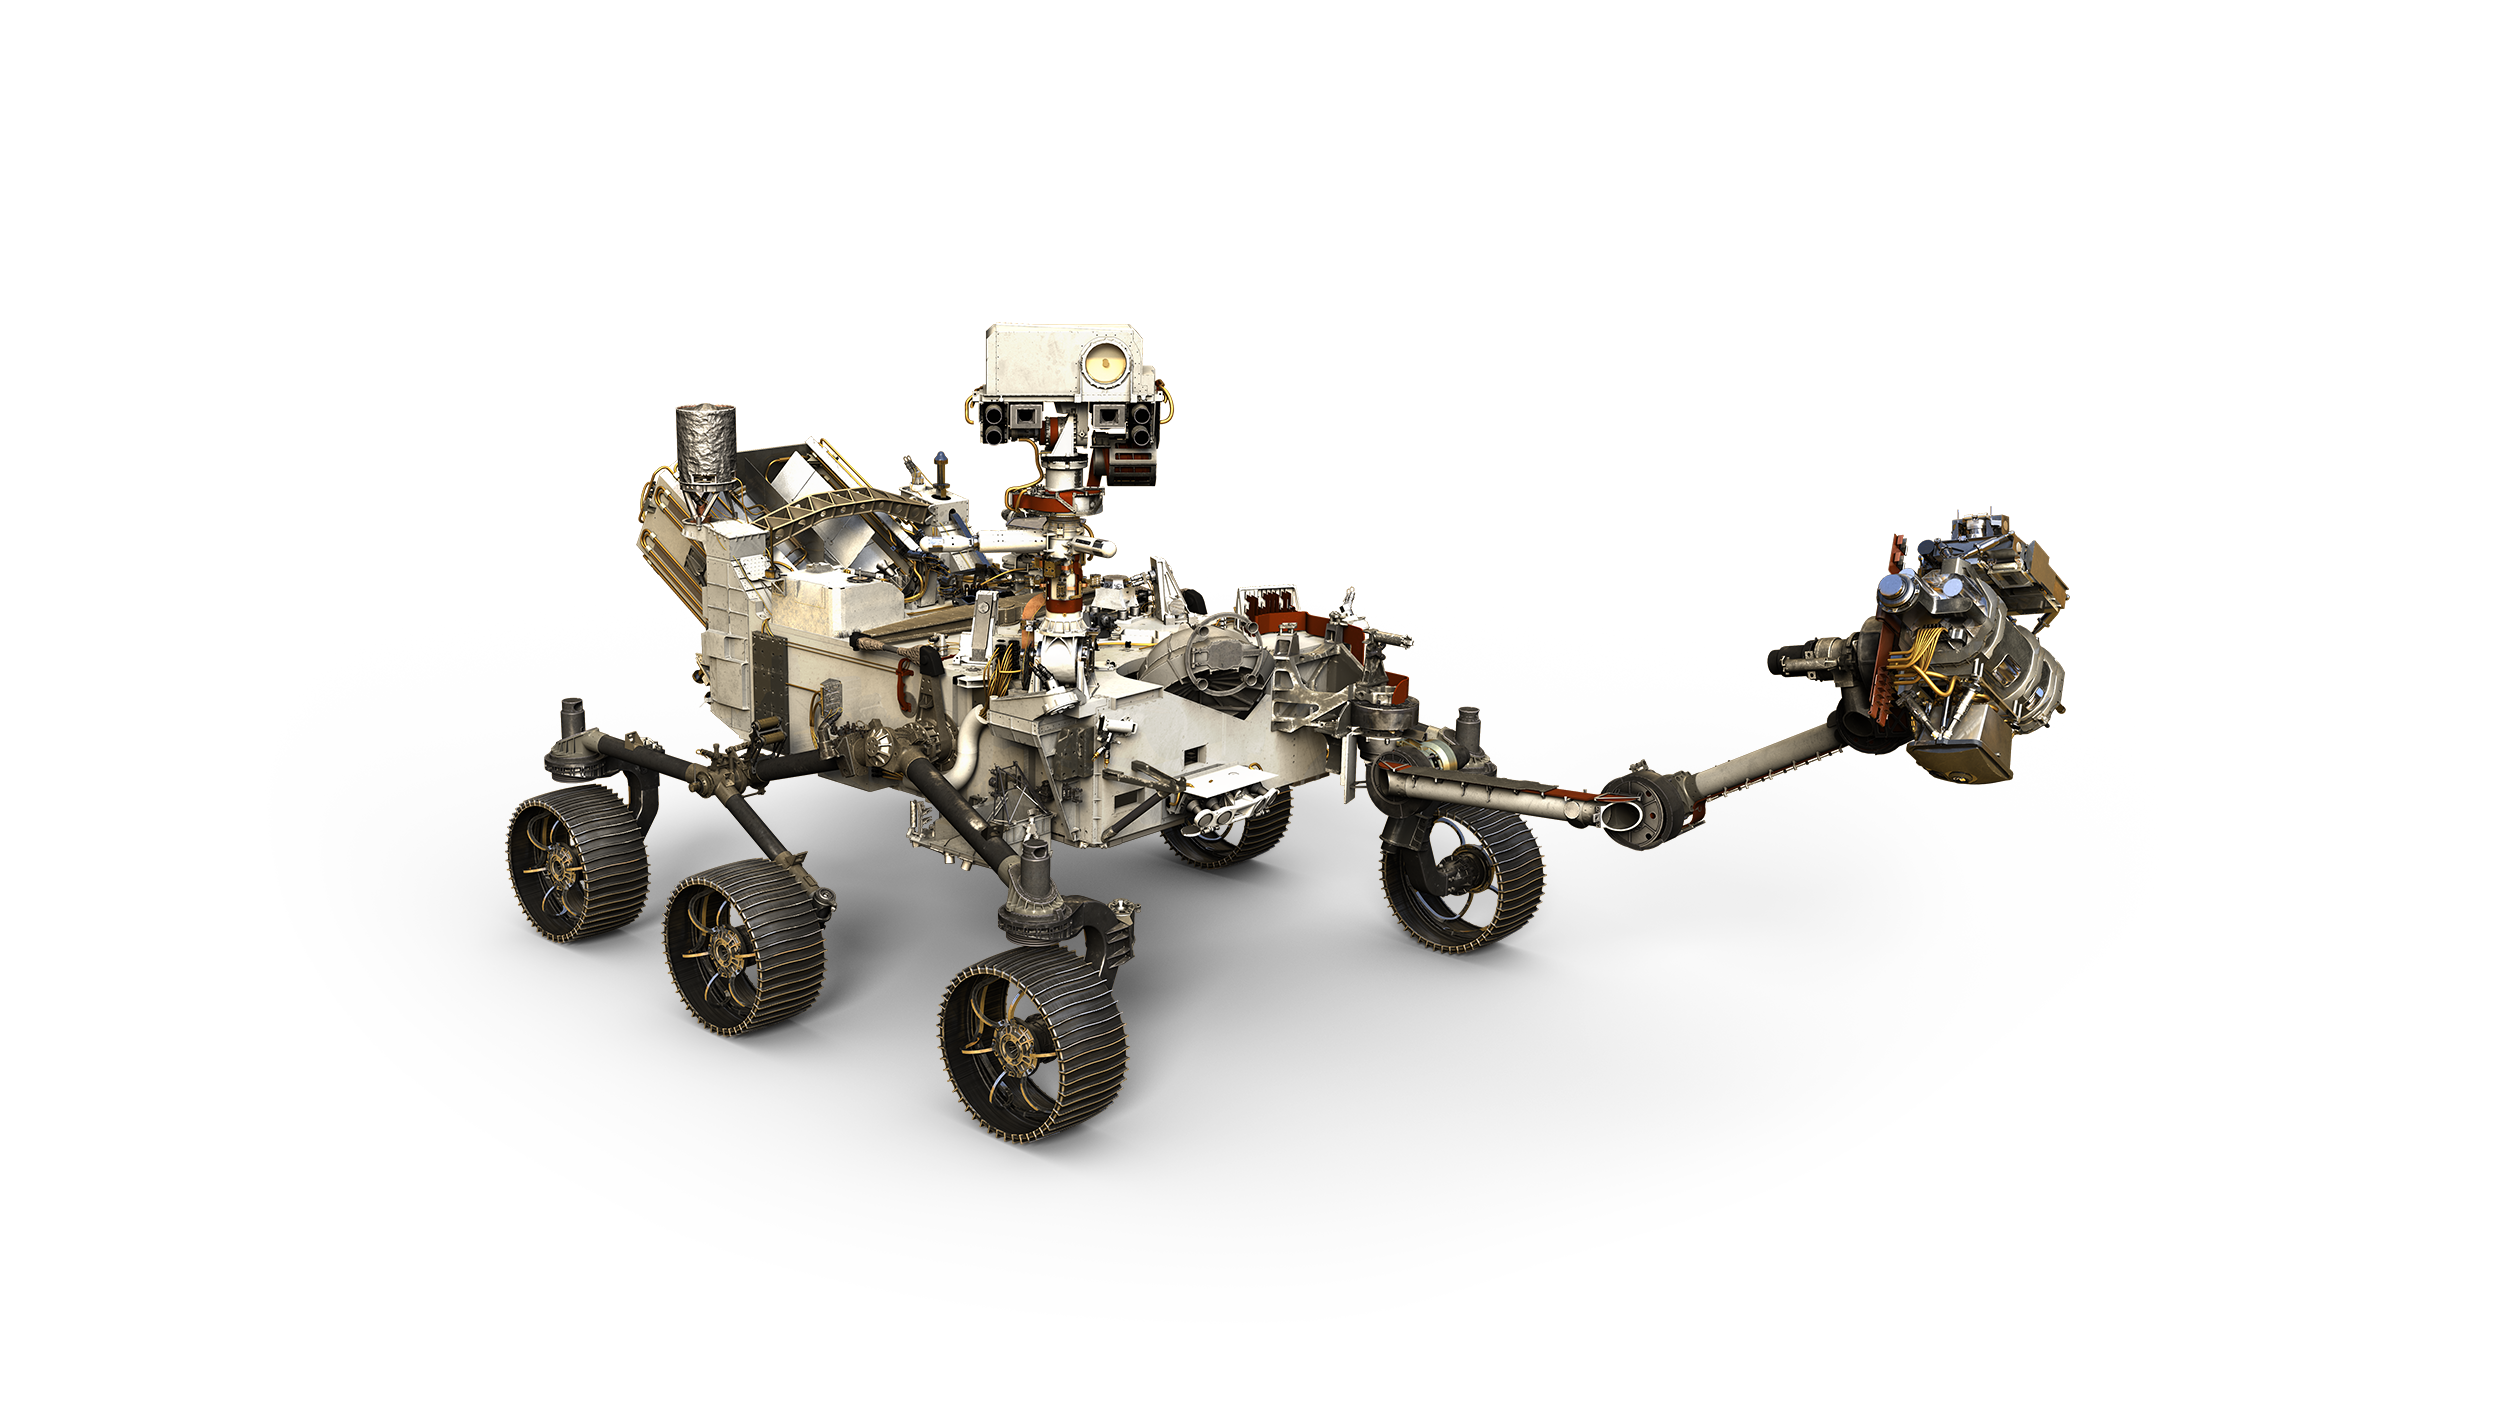
\includegraphics[scale=0.15]{JPL_rover}
	\caption{JPL Rover designed for Mars2020 mission}
\end{figure}
In industry too automated robotic systems are used in order to achieve:
\begin{itemize}
	\item A better production quality, having the possibility to more easily measure and control the performances;
	\item Improved productivity, reducing downtimes and the consumption of resources;
	\item Robots can have access to environments which are too risky or not accessible for humans;
	\item Robots maintenance can be much cheaper than other man-driven alternatives. 
\end{itemize}
In this sense mobile robotics is a very practical example of how the efficiency of a plant can be improved, reducing the effort for the trasportation tasks, or collecting datas from a warehouse automatically, or in many other ways.\\
However, when in the early '90s people has started mounting manipulator arms on mobile platforms, the resulting system opened the research to endless possibilities. These systems are now called Mobile Manipulators.
The mobility of robots substantially increased what they can cope. Robots are now expected to explore unknown dynamic environments, interact with human beings or manipulate hazardous products. Mobile manipulators are systems that combine locomotion and manipulation capabilities in order to fulfil such missions. \\
Except for some special types of Mobile Manipulators like:
\begin{itemize}
	\item Submarine Mobile Manipulators for underwater applications;\begin{figure}[h!]
		\centering
		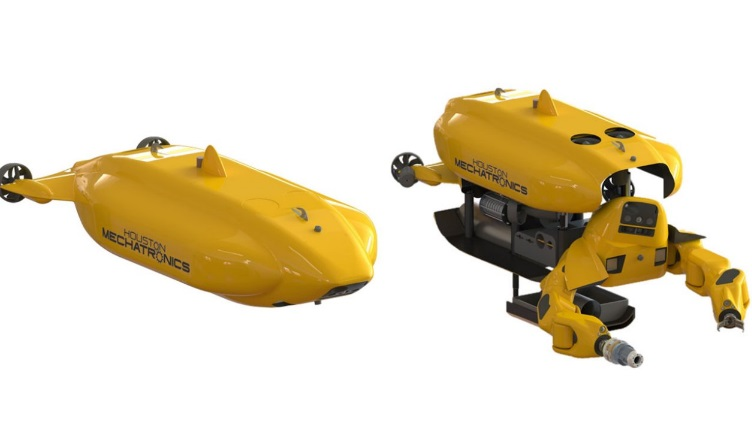
\includegraphics[scale=0.3]{submarine_robot}
		\caption{Houston Mechatronics's Aquanaut}
		\label{fig:aquanaut} 
	\end{figure}
	\item Legged humanoid or animal-like robots for service missions;\begin{figure}[h!]
		\centering 
		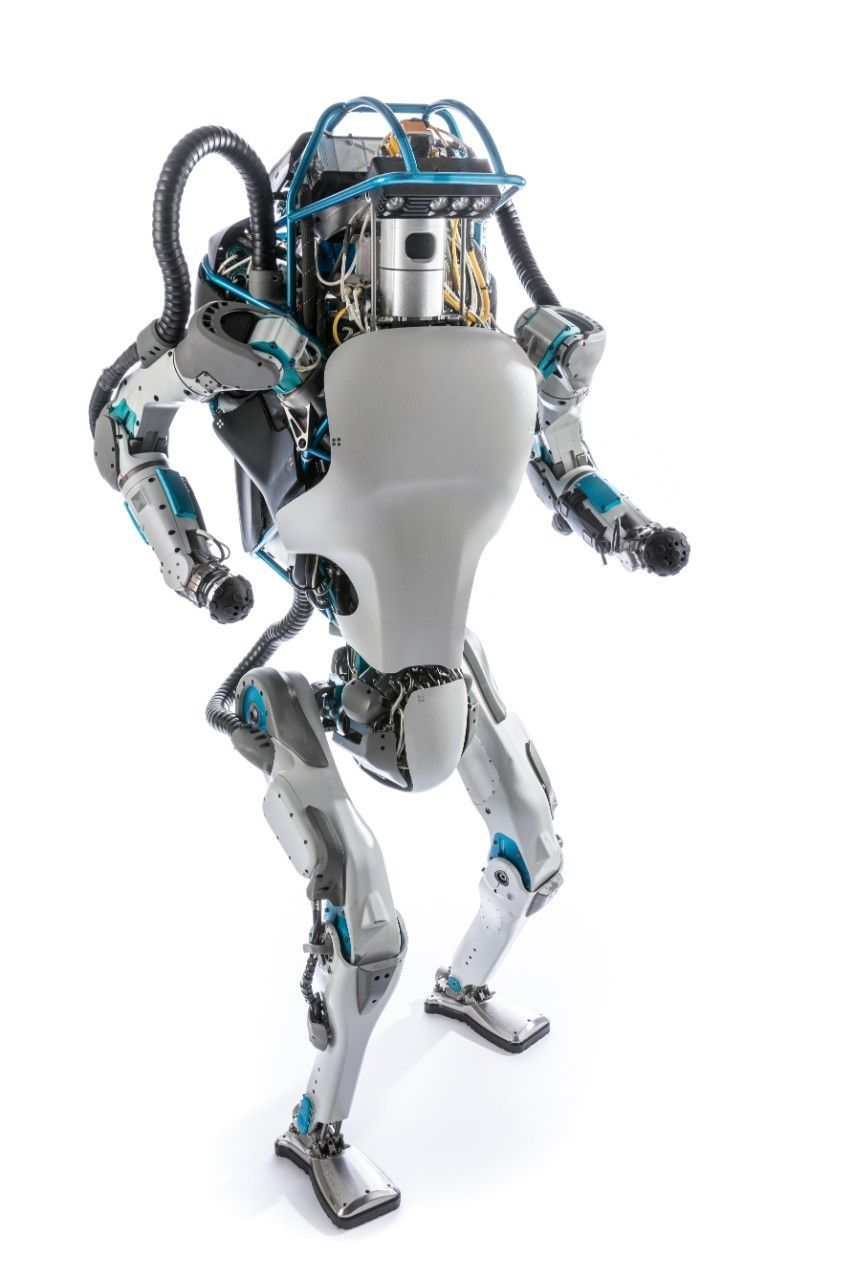
\includegraphics[scale=0.095]{atlas}
		\label{fig:atlas} 
		\quad
		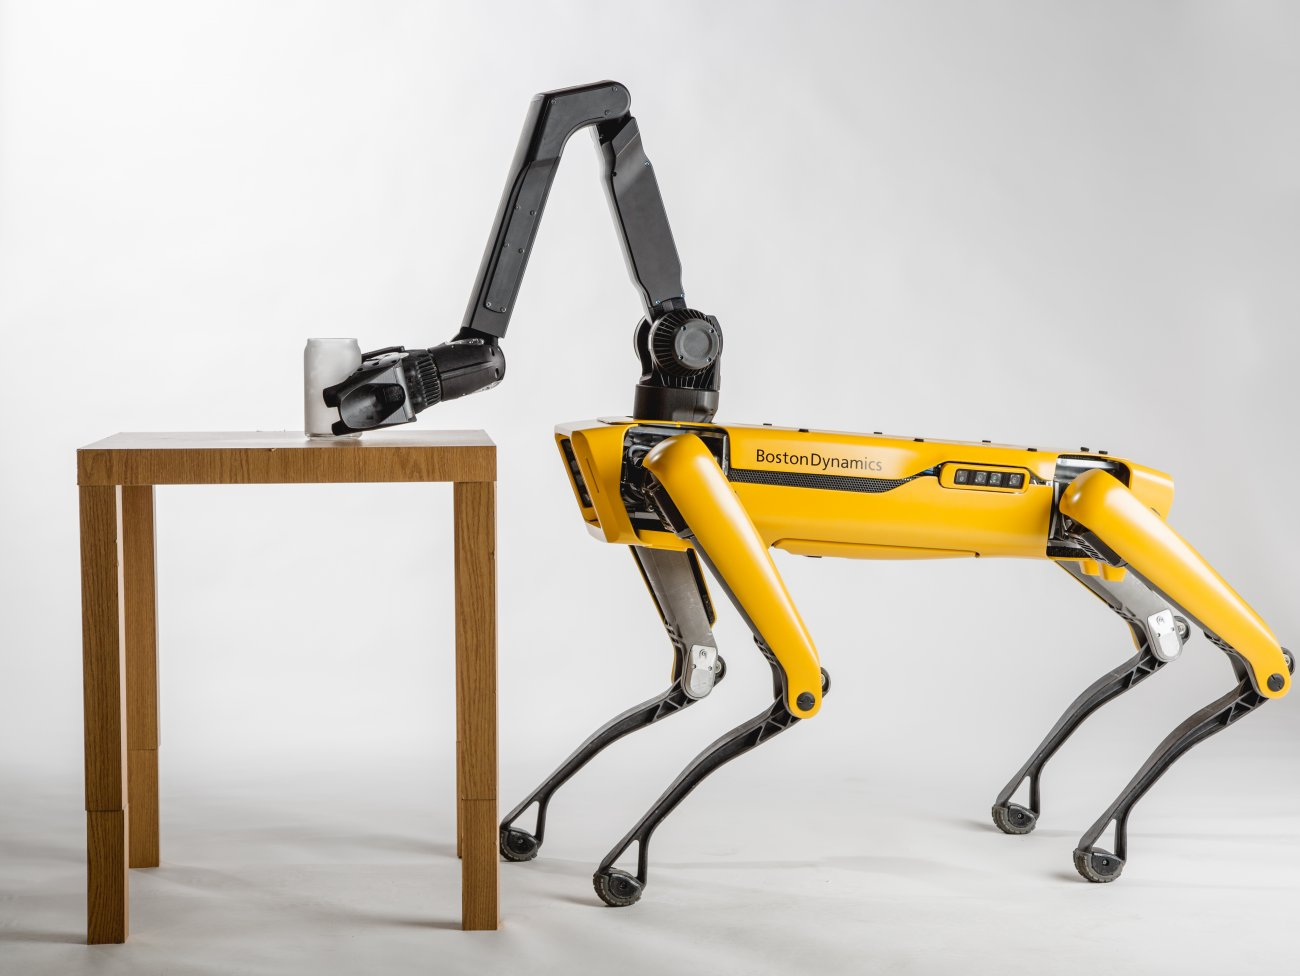
\includegraphics[scale=0.10]{spot_mini}
		\label{fig:spotmini} 
		\caption{Boston Dynamics's Atlas and Spot Mini}
	\end{figure}
	\item Omnidirectional vehicles \begin{figure}[h!]
		\centering
		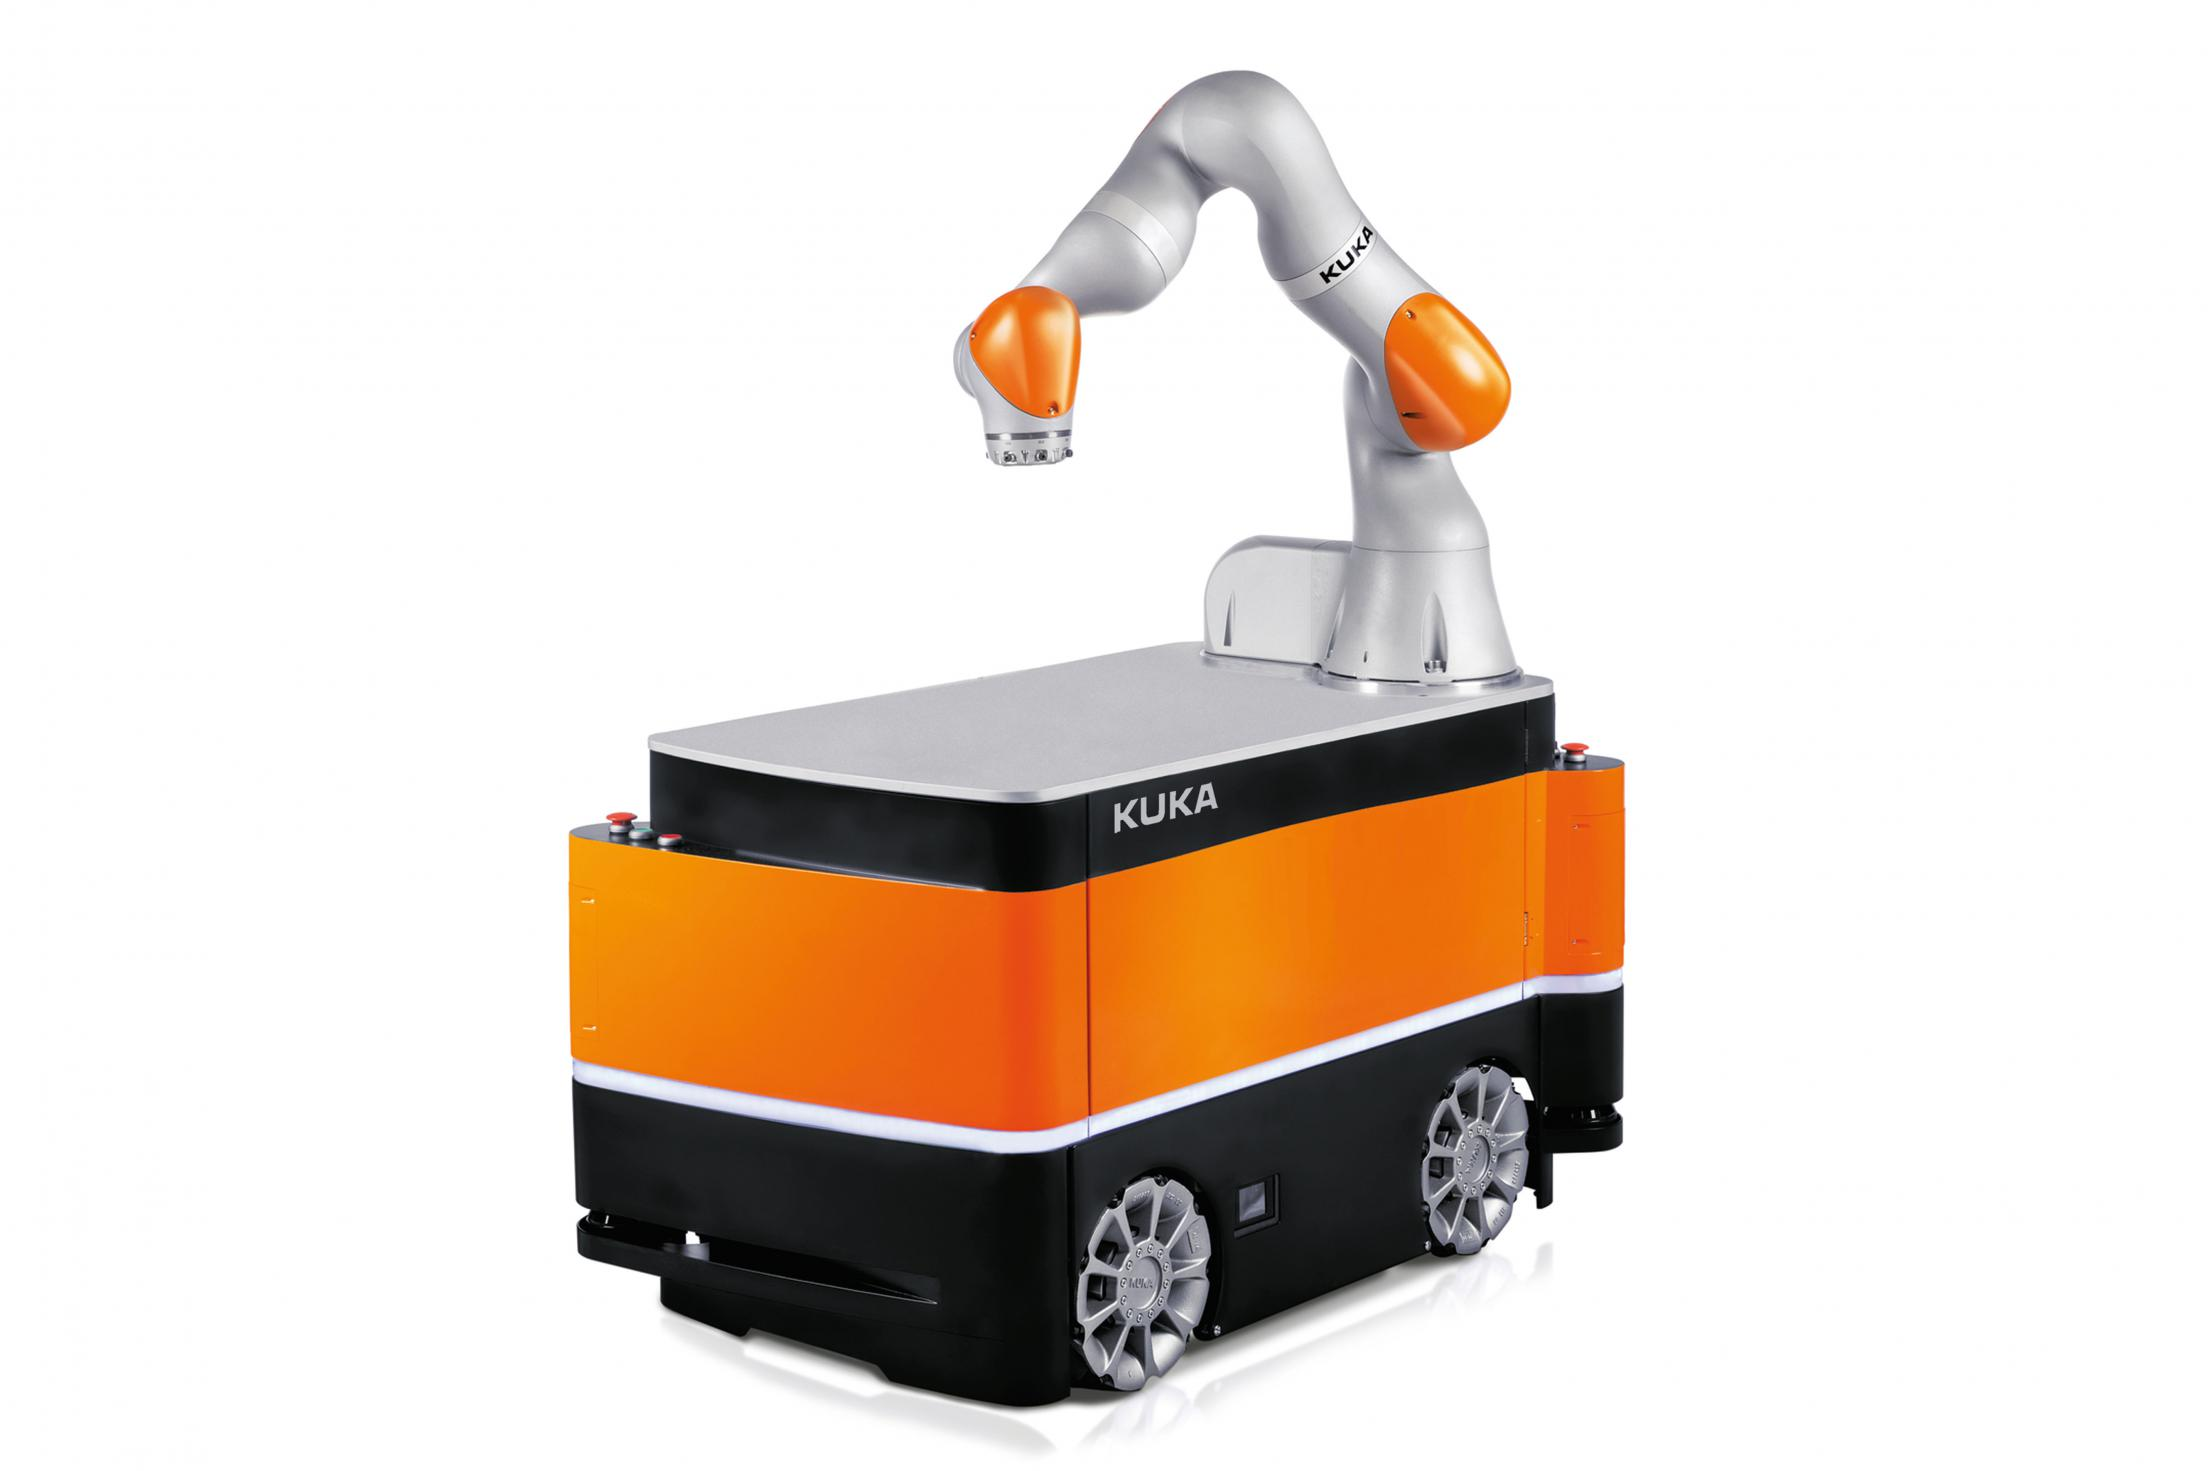
\includegraphics[scale=0.095]{kuka_iiwa}
		\caption{Kuka KMR iiwa: a Mobile Manipulator with omnidirectional wheels}
		\label{fig:iiwa} 
	\end{figure}
\end{itemize}
Mobile Manipulators combine a nonholonomic wheeled mobile base and one or more robotic arms. From a physical point of view the presence of the base makes the entire Mobile Manipulator a nonholonomic system, meaning a system described by a set of variables subjected to differential constraints. Nonholonomic constraints will be better explained in Chapter \ref{chapter2}. The same chapter is also devoted to the kinematic and dynamic description of wheeled Mobile Manipulators, mainly pointing to two important aspects:
\begin{enumerate}
	\item The entire system is often kinematically redundant with respect to the task to be achieved;
	\item The dynamic properties of the base are very different from the manipultor ones.
\end{enumerate}
After a brief introduction about the theory of control strategies in Chapter \ref{chapter3}, Chapter \ref{chapter4} can be referred for a fairly thorough summary of Mobile Manipulator control; even if Mobile Manipulators are a technology known from the early 90s, just a little can be found in literature on this topic. In particular, except for very few cases, MPC control has been applied only with holonomic Mobile Manipulators. This is due to the fact that this kind of control requires high computational effort, especially with highly nonlinear systems like Mobile Manipulators. MPC is a powerful tool to face all the constraints on Mobile Manipulators motion that have to be taken into account: obstacle avoidance, self collision avoidance, joint limits, joint speed limits, singular configurations avoidance, etc. exploiting also the kinematic redundancy of the system.\\
In Chapter \ref{chapter5} we present the architecture of an online MPC control for a nonholonomic Mobile Manipulator in order to achieve a trajectory following task for the manipulator's end effector while coping with the constraints previously mentioned. In Chapter \ref{chapter6} experimental results are presented and eventually in Chapter \ref{chapter7} conclusions are drawn highlighting our main contributions and future work.	

\section{Objective of the thesis}
The main objective of this thesis is to design a controller for a Nonholomic Mobile Manipulator able to perform trajectory tracking for motion and grasping operations in unstructured enviroments. The trajectories are given as end effector position and orientation in time in order to perform grasping of objects in a time-optimal manner. The planning algorithm presented in \cite{shantanuthakar} precomputes the optimal trajectories to perform a specific task, although the algoritm is not suitable for online implementation because of the high execution time. The design of an online controller is then required, also to take into account unexpeted events and positioning errors of the end effector. The main issue related to the developement of such a controller lies in the non linearity of the model and the high redundancy of the system itself. For those reasons a control technique that allows to take into account unforseen events, manipulability and constraints on the system has to be identified. The complexity of the problem and the variety of tasks requires to use a hierarchical approach and, given that low level loops are provided by manufacurers, to find a suitable high level control logic. The field of control for mobile manipulator is nowdays of great interest because of the increased possibilities and requirements in industrial applications.  




%!TEX root = Thesis_main.tex

\chapter{Kinematic Model of the Mobile Manipulator}
\label{chapter2}
\section{Mobile Robot Model}
\subsubsection{Holonomic and Nonholonomic constraints}
Constraints which reduce the dimensions of the accessible configuration space of a system of rigid bodies, i.e. acting on the generalized coordinates $x$ that describe the system, are said to be \textit{holonomic} or integrable. 
Holonomic constraints are expressed in the form:
\begin{equation}
h\left( x\right) =0
\end{equation}
All constraints which instead are nonintegrable are said to be \textit{nonholonomic}, so also inequality constraints on the configuration space. In particular, constraints on the generalized velocities of the system of rigid bodies but not on its configuration are nonholonomic.\\
Nonholonomic constraints reduce the mobility of the mechanical system in a completely different way with respect to holonomic constraints. The fact that the constraint is nonintegrable means that there is no loss of accessibility to the entire configuration space for the system. In other words, while the subspace of the generalized velocities is reduced due to the constraint, the number of generalized coordinates cannot be reduced.
Nonholonomic constraints are expressed in the form:
\begin{equation}
h( x,\dot{x}) =0
\end{equation}
Kinematic constraints both holonomic or nonholonomic are usually written in the Pfaffian form, i.e. linearly with respect to the generalized velocities.
\begin{equation}
a_i^T \left( x \right)\dot{x} =0 \qquad i=1,...,k<n 
\end{equation}
or in a compact form:
\begin{equation} 
A^T \left( x \right)\dot{x} =0  
\end{equation}
Assuming now to have $k$ nonholonomic constraint equations for a $n$ dimensional system, this implies that the admissible generalized velocities $\dot{x}$ of the system in any of its configuration $x$ necessarily belong to a $(n-k)$-dimensional space. Specifically, expressing the constraint equations in Pfaffian form, the generalized velocities should belong to the null space of matrix $A^T$.\\
Thus, it can be written as
\begin{equation} \label{G}
\dot{x}=\sum_{j=1}^{m} g_j(x)u_j=G(x)u \qquad m=n-k
\end{equation}
where $x\in \mathbb{R}^n $ is the vector of the generalized coordinates describing the system (state vector), $u= \left[
\begin{matrix}
u_1 &  \cdots & u_m
\end{matrix}
\right]^T\in\mathbb{R}^m $ is the input vector and $\left\lbrace  g_1(x) \cdots g_m(x) \right\rbrace $ is a basis of the null space of $A^T$.\\ 
Talking about mobile robots, wheels are by far the most common mechanism to achieve locomotion. Any wheeled vehicle is subject to kinematic pure rolling constraints that reduce in general its local mobility, while leaving intact the possibility of reaching arbitrary configurations by appropriate manoeuvres. The pure rolling constraint is nonholonomic, because it implies no loss of accessibility in the configuration space of the vehicle.\\
The kinematics of a wheeled mobile robot subjected to pure rolling constraints changes depending on how locomotion is achieved. Mainly there are two types of wheeled mobile robot models: unicycle like robots and bicycle like ones. We will focus on the first one.
\subsubsection{Unicycle Model}
\begin{figure}[h!]
	\centering
	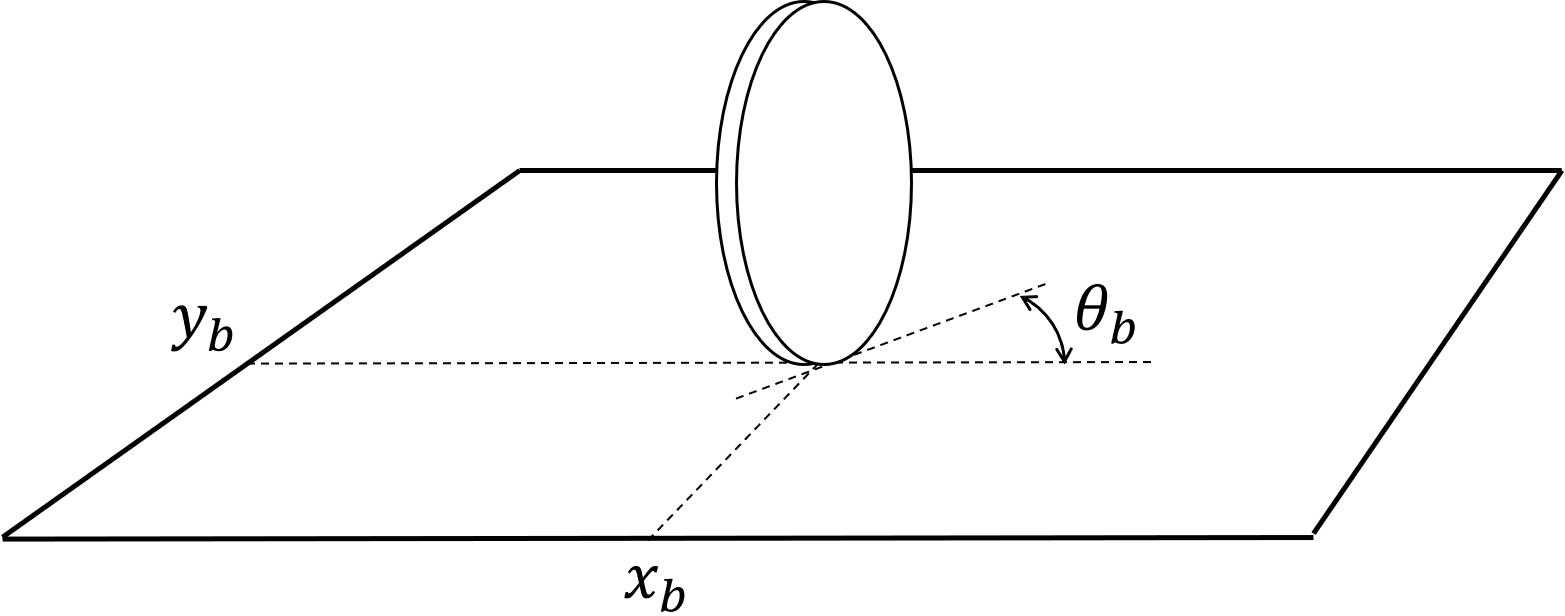
\includegraphics[scale=0.4]{unicyclemodel}
	\caption{Unicycle model}
	\label{fig:unicyclemodel}
\end{figure}
A unicycle is a vehicle whose configuration is completely described by the configuration vector $x = \left[\begin{matrix}x_b&y_b&\theta_b\end{matrix}\right]^T$, where $x_b$ and $y_b$ are the Cartesian coordinates of the contact point of the wheel with the ground and $\theta_b$ is the orientation of the wheel with respect to the axis of the abscissas, as showed in figure \ref{fig:unicyclemodel}. \\
The pure rolling constraint for the unicycle is simply expressed as:
\begin{equation} \label{At}
\dot{x}_b\sin\theta_b-\dot{y}_b\cos\theta_b=\left[
\begin{matrix}
\sin\theta_b & \cos\theta_b & 0
\end{matrix}
\right] \dot{x}= A^T \left( x \right)\dot{x} =0  
\end{equation}
This equation expresses that the velocity of the contact point (or of the wheel centre) is zero in the direction orthogonal to the sagittal plane of the disk.\\
Hence the unicycle is a 3-dimensional system subject to one nonholonomic constraint, so the dimension of the basis of the null space of $A^T$ is 2. Choosing:
\begin{equation} \label{Gmatrix_def}
G(x)=\left[
\begin{matrix}
g_1 (x) & g_2 (x)
\end{matrix}
\right] =  \left[
\begin{matrix}
\cos\theta_b & 0 \\
\sin\theta_b & 0 \\
0 & 1 
\end{matrix}
\right] 
\end{equation}
All the generalized velocities of the unicycle at $x$ are a combination of $g_1 (x)$ and $g_2 (x)$.
\begin{equation} 
\dot{x}=\left[
\begin{matrix}
\dot{x}_b \\ \dot{y}_b \\\dot{\theta}_b
\end{matrix}
\right] =  \left[
\begin{matrix}
\cos\theta_b \\ \sin\theta_b \\ 0 
\end{matrix}
\right]v + \left[
\begin{matrix}
0 \\ 0 \\ 1 
\end{matrix}
\right]\omega
\end{equation}
Where $v$ is the driving velocity, i.e. the velocity of the disk along its sagittal plane, and $\omega$ is the steering velocity, i.e. the angular speed around its vertical axis.\\
A lot of mobile robots are kinematically equivalent to a unicycle, like differential drive robots, like the one in figure \ref{fig:mobilebase}, skid steering robots or synchro drive vehicles.\\
In most of the unicycle-like mobile robots, $v$ and $\omega$ are the command input to the system, while the actual velocity input are $\omega_R$ and $\omega_L$, i.e. the right and left wheels angular speeds: 
\begin{equation}
v=\frac{r\left(\omega_R + \omega_L\right)}{2} \qquad \omega=\frac{r\left(\omega_R - \omega_L\right)}{d}
\end{equation}
\begin{equation}
\omega_R =\frac{1}{r}\left(v+\frac{d}{2}\omega\right) \qquad \omega_L=\frac{1}{r}\left(v-\frac{d}{2}\omega\right)
\end{equation}
where $r$ is the wheel radius and $d$ is the distance between their centres.
\begin{figure}[h!]
	\centering
	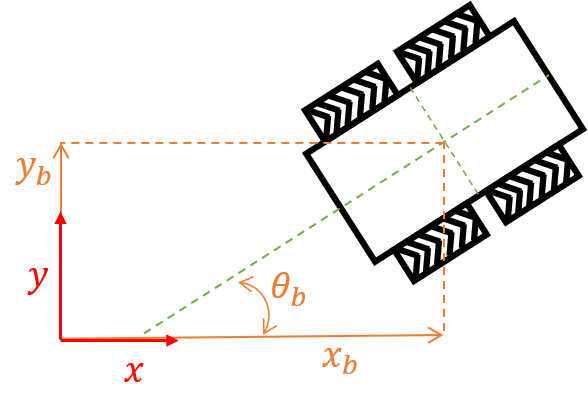
\includegraphics[scale=0.8]{mobilebase}
	\caption{Scheme of a Differential Drive Mobile Robot}
	\label{fig:mobilebase}
\end{figure}
\section{Manipulator Model}
A manipulator consists of a series of rigid links connected by joints. Mathematically it can be modeled as a kinematic chain where one end of the chain is constrained to a base, while an end effector is mounted to the other end. The end effector is used to manipulate objects in space. Therefore, it is the end effector position and orientation, \textit{pose}, that is often studied. \textit{Forward kinematics} describes the pose of the end effector as a function of the joint values:
\begin{equation}
 	\xi=\left[\begin{matrix}p_{EE}\\\Phi\end{matrix}\right]=f(x)
\end{equation} 
where $p_{EE}=\left[\begin{matrix}x_{EE}&y_{EE}&z_{EE}\end{matrix}\right]^T$ is the vector of the end effector position and $\Phi =\left[\begin{matrix}\vartheta_{EE}&\varphi_{EE}&\psi_{EE}\end{matrix}\right]$ is the vector of the end effector orientation expressed with different conventions like Azimut-Elevation-Rotation, or Roll-Pitch-Yaw. 
It is possible to express this relation in a compact form using the homogenous \textit{rototraslation matrix} $A_{ee}^{base}$ that describes the end effector reference frame with respect to the base global reference frame:
\begin{equation}\label{AAAA_man}
A_{ee}^{base}=A_1^{base}A_2^1A_3^2\cdots A_{ee}^{ee-1}
\end{equation}
where $A_i^{i-1}$ is the expression of the transformation from one joint frame to the following one through the use of Denavit-Hartemberg parameters \cite{DH}: $a\text{, }\alpha\text{, }d\text{, }\theta$ (defined as in figure \ref{fig:DH}):
\begin{equation}
A_i^{i-1}(q_i)=\left[
\begin{matrix}
\cos\theta & -\sin\theta\cos\alpha & \sin\theta\sin\alpha & a\cos\theta \\
\sin\theta & \cos\theta\cos\alpha & -\cos\theta\sin\alpha & a\sin\theta \\
0 & \sin\alpha & \cos\alpha & d \\
0 & 0 & 0 & 1
\end{matrix}
\right]
\end{equation}
This matrix is function only of the joint variables $\theta$ and $d$.

\begin{figure}[h!]
	\centering
	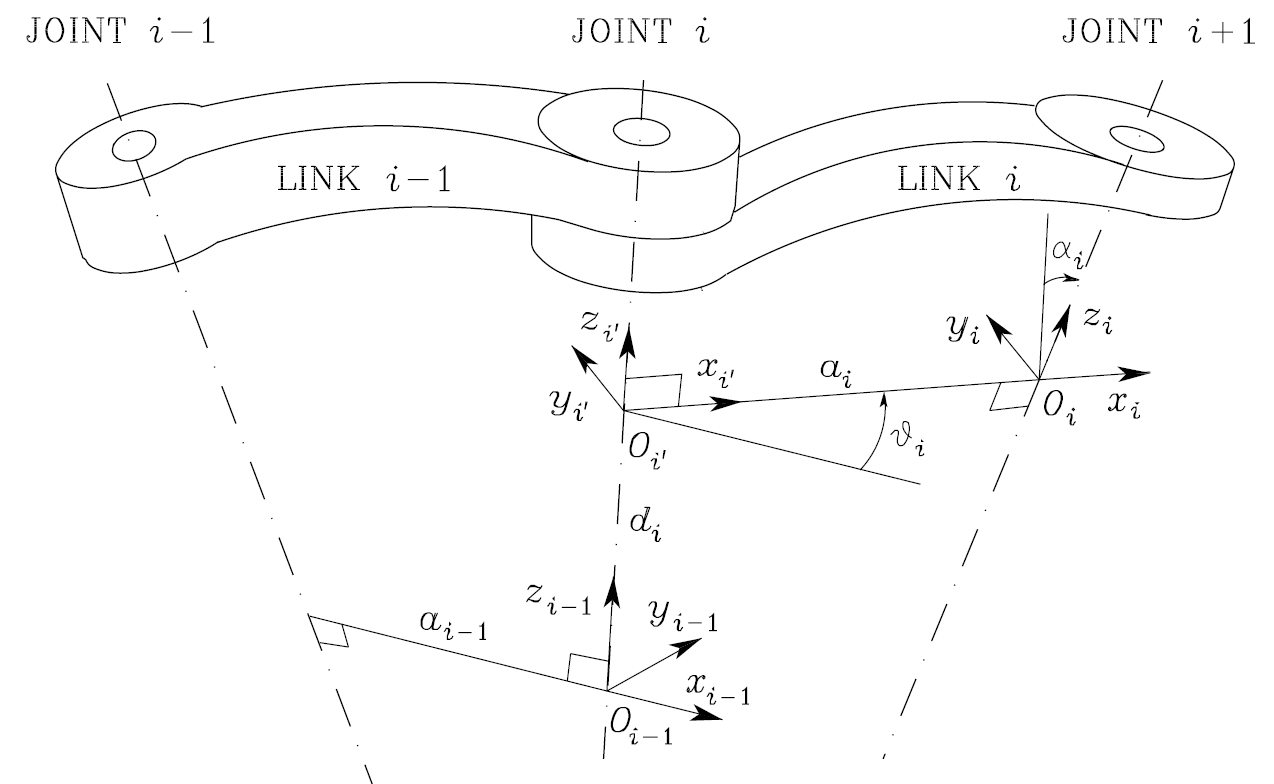
\includegraphics[scale=0.4]{denavithartenberg}
	\caption{Denavit-Hartenberg convention for Robot links}
	\label{fig:DH}
\end{figure}

The opposite problem is the definition of the \textit{inverse kinematics}, i.e. given the position and orientation of the end effector, finding the corresponding joint variables. The inverse kinematics problem is not easy to solve since it is often nonlinear and there can be infinite solutions as well as none.\\
An important concept which roboticists are still working on is \textit{kinematic redundancy}, i.e. when the number of joint variables is greater than the dimension of the operational space relative to the task to be achieved. For example, for a problem of end effector position and orientation regulation the task operational space is 6-dimensional.
When a system is kinematically redundant, direct kinematics is always possible to be defined, while inverse kinematics can have infinite solutions.
Solving the \textit{kinematic redundancy problem} means to define a criterion in order to be able to pick one among the infinite configurations which have the end effector in the same position and orientation.\\
This concept will be very important in the defintion of Mobile Manipulator control, since Mobile Manipulators are highly redundant systems.

\section{Mobile Manipulator Model}
\begin{figure}
\centering
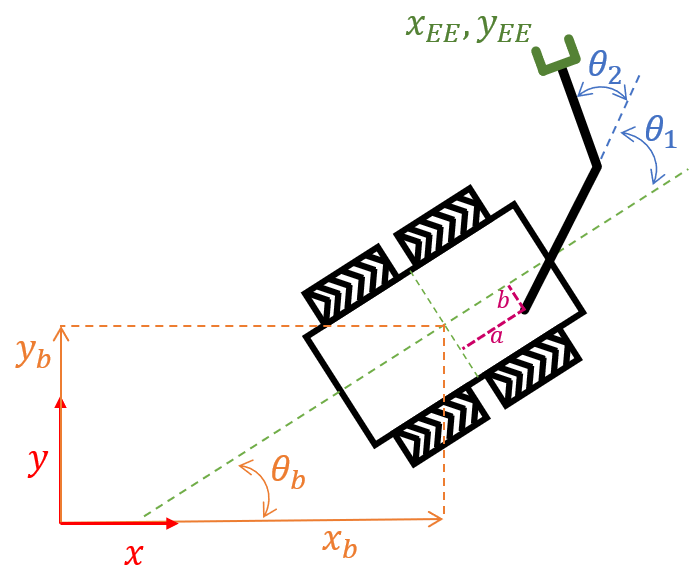
\includegraphics[scale=0.8]{MMkinematics}
\caption{A simple Mobile Manipulator composed by a mobile base and a 2-Dof robotic arm}
\label{fig:MMkinematics}
\end{figure}
Considering the general case of a mobile manipulator composed by a manipulator arm mounted on a mobile platform, its kinematic model set the location and orientation of the end effector as a function of both the arm and base generalized coordinates:
\begin{equation}\label{dirkinMM}
	\xi=\left[\begin{matrix}p_{EE}\\\Phi\end{matrix}\right]=f(x)=f\left(\left[\begin{matrix}x_{base}\\x_{arm} \end{matrix}\right]\right)
\end{equation}
where $x_{base}$ is the configuration vector of the mobile base and $x_{arm}$ is the vector of joint coordinates of the manipulator.
As an example, the forward kinematics for just the Cartesian coordinates of the end effector of the simplified system in figure \ref{fig:MMkinematics} is
\begin{equation*}
\begin{split}
	x_{EE}&=x_b+a\cos\theta-b\sin\theta+l_1\cos\left(\theta+\theta_1\right)+l_2\cos\left(\theta+\theta_1+\theta_2\right)\\
	y_{EE}&=y_b+a\sin\theta-b\cos\theta+l_1\sin\left(\theta+\theta_1\right)+l_2\sin\left(\theta+\theta_1+\theta_2\right)
\end{split}
\end{equation*}
It is possible to express the function $f(x)$ of Eq.\ref{dirkinMM} as in \ref{AAAA} premultiplying the rototranslation matrix $A_{base}^{global}$, relative to the mobile base motion, to the direct kinematics of the arm. In the case of the previous example:
\begin{equation}
	A_{base}^{global}=\left[\begin{matrix}
		\cos\theta&-\sin\theta&0&x_b+a\cos\theta-b\sin\theta\\
		\sin\theta&\cos\theta&0&y_b+a\sin\theta-b\cos\theta\\
		0&0&1&h_{base}\\
		0&0&0&1
	\end{matrix}\right]
\end{equation}
So the forward kinematics can be obtained consequently:
\begin{equation}\label{AAAA}
A_{ee}^{global}=A_{base}^{global}A_1^{base}A_2^1\cdots A_{ee}^{ee-1}
\end{equation}
\paragraph{Redundancy}
As we had briefly introduced before, a robot is kinematically redundant if the number of its degrees of freedom is greater than it is strictly necessary. In this sense redundancy is thus a concept relative to the given task. Mobile Manipulators are systems specifically built redundant in order to exploit the extra degrees of freedom to:
\begin{itemize}
	\item avoid collision with obstacles;
	\item avoid kinematic singularities;
	\item increase the manipulability of the system;
	\item move with lower joint velocities;
	\item etc.
\end{itemize}
A common way to deal with redundant systems is to move the problem at velocity level through the use of Jacobians, as we will see more in detail in the following chapters. 
\paragraph{Differential kinematics}Differentiating $f$, the differential forward kinematics of the Mobile Manipulator can be obtained:
\begin{equation}\label{eq:dotx_EE}
	\dot{X}_{EE}=\mathcal{J}_b(x)\dot{x}_{base}+\mathcal{J}_a(x)\dot{x}_{arm}
\end{equation}
where the columns of $\mathcal{J}_a(x)={\partial f}/{\partial x_{arm}}(x)$ can be obtained as:
\begin{equation}
\mathit{j}_{P_j}^{(EE)}=
	\begin{cases}
	z_{j-1} & \text{for a \textit{prismatic} joint} \\
	z_{j-1}\times \left(p_{EE}-p_{j-1}\right) & \text{for a \textit{revolute} joint}	
	\end{cases}                                             
\end{equation}
\begin{equation}
	\mathit{j}_{O_j}^{(EE)}= 
	\begin{cases}
	0 & \text{for a \textit{prismatic} joint} \\
	z_{j-1} & \text{for a \textit{revolute} joint}	
	\end{cases} 
\end{equation}
and $\mathcal{J}_b(x)={\partial f}/{\partial x_{base}}(x)$ can be obtained at the same way considering $x_b$ and $y_b$ as prismatic joints and $\theta_b$ as a revolute joint of the compound system.\\
In this the nonholonomic constraint \ref{G} of the mobile platform should be taken into account:
\begin{equation}
	\mathcal{J}_b(x)\dot{x}_b=\mathcal{J}_b(x)G(x)v=\mathcal{J}_v(\theta_b)v
\end{equation}
Therefore is now possible to reformulate eq \ref{eq:dotx_EE} in a compact form to express the end effector traslational and rotational velocities as a function of the 8-elements input vector of joints and vehicle velocities.
\begin{equation}
\dot{X}_{EE}=\left[\begin{matrix}
\mathcal{J}_v(\theta_b) & \mathcal{J}_a(x)
\end{matrix}\right]\left[\begin{matrix}v\\\dot{x}_{arm} \end{matrix}\right] = \mathcal{J}(x)\dot{x}
\end{equation}


%!TEX root = Thesis_main.tex

\chapter{Control Theory}
\label{chapter3}

The interconnection between control theory and robotics has a history that of over half a century during which control theory has developed solutions problems in robotics field and problems in robotics have gained the new control theories. In the last decade or two, the Progress in robotic systems has been rapid, especially thinking about the applications increase, from machine tool industry to biomedical applications for example. The early design of robotic systems was to develop mechanisms to be as stiff as possible modeled as single-input/single-output (SISO) linear systems with each joint controlled independently. Then Point-to-point control used to perform simple tasks such as spot welding or pick and place operations. Encoureged by industry request, more complex tasks such as arc welding and spray painting has been enabled from Continuous-path tracking. But to consider more advanced tasks like assembly was restricted by the limited or nonexistent sensing of the external environment. Higher speeds and higher payload-to-weight ratios required a better understanding of modeling of nonlinear dynamical systems. For this reason new theoretical results in nonlinear, robust, and adaptive control enabled more advanced applications. Today, robot control systems are highly advanced with integrated sensing systems. Robot networks, surgical robots, mobile robots, underwater and flying robots, and others are starting to play important roles in society.
\section{PID Control}

PID architecture is the most common form of feedback controllers. The first implementation of PID controllers dates back to early 20th century. Today more than 90 \% of the control loops are PID type and are found in many areas. Nowdays is often combined with other advanced control techniques where generally the main usage of PID based controllers is for low level loops like motor controllers, integrated circuits etc. while advanced techniques are used for high level control.
When dealing with mobile robots, which are generally designed to perform tasks more or less autonomously, the aim of the controller can be manifold. In the case of mobile robots for pick and place operation the architecture of the online controller is generally hierarchic and the role of the PID regulator is to track desired high level control input.
\\ 
\\ The general control law for a PID controller is defined as follows: 

\begin{equation}
	p( t) = K_P e(t) +K_I\int\limits_{0}^{t} e(\tau)d\tau + K_D \frac{de(t)}{dt}
\end{equation}
The advantages of this basic control logic is the simplicity of implementation, lucid meaning, and the near-zero memory usage from the phisical hardware. Because of that and the many tuning techniques developed in years PID as been widely accepted in industry. Anyway this basic feedback control law present consisten limitation for andvanced applications. The goal of this type of controllers is to define a control law able to reduce the errors computed by means of the given measured data, so it works going after the real system measured outputs. The tuning of the controller is made chosing the parameters $K_P$, $K_I$ and $K_D$ that change the response of the closed loop system. Those parameters have to be chosen properly in order to achive stability and performances. Nevertheless, it's generally not possible to take into account any changes in the system dynamic. Because of that other control techniques have been developed in years.


\section{Inverse Dynamics Control}

The inverse dynamics control approach is directly related to the solution of the inverse dynamics problem of the system. Given the specified motion and the desired properties of the resulting system, the control inputs that ensure stability and realization of these control objectives are to be found. By appropriately inverting the dynamic model of the system to be controlled, a control law can be found. Generally this control law is chosen in order to cancel out the nonlinear part of the dynamics, to decouple the interactions between the regulated variables, and specify the behaviour of the convergence of the error. The inverse dynamics controller is able to enforce the execution of prescribed motion of the system and at the same time to control the interaction forces with the environment. If we consider a generic dynamical system in the form:
\begin{equation}
	H(q)\ddot{q}+C(q,\dot{q})\dot{q}+\tau_g(q)=\tau	
\end{equation}
The inverse dynamics control law can be defined: 
\begin{equation}
	\tau=H(q)v+C(q,\dot{q})\dot{q}+\tau_g(q)
\end{equation}
From this control law results that $\ddot{q}=v$. Where $v$ is a new conrol input, one approach to define it is with a PD (Proportional-Derivative) feedback:
\begin{equation}
	v = \ddot{q}_d+K_V\dot{e}_q+K_Pe_q
\end{equation}
The overall control input becomes:
\begin{equation}
	\tau=H(q)(\ddot{q}_d+K_V\dot{e}_q+K_Pe_q)+C(q,\dot{q})\dot{q}+\tau_g(q)
	\label{inverse_dyn_cont_law}
\end{equation}
So the resulting error dynamics is linear:
\begin{equation}
	\ddot{e}_q+K_V\dot{e}_q+K_Pe_q=0
\end{equation}
That is, properly choosing $K_V$ and $K_P$ parameters theconvergence of the error is zero.  
\\\
\begin{figure}
	\centering
	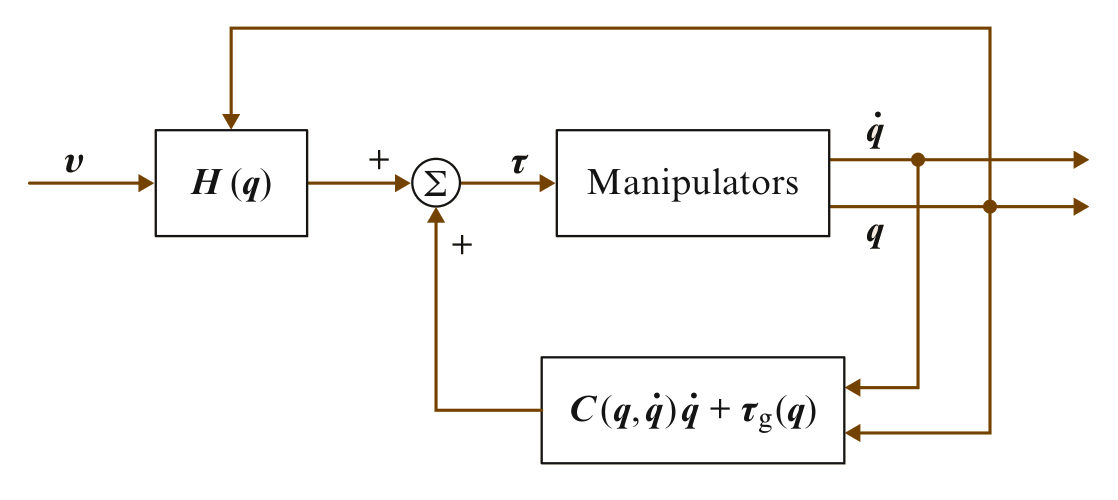
\includegraphics[scale=0.3]{torque_control}
	\label{Torque_control_scheme}
	\caption{Inverse dynamics control scheme}
\end{figure}
The usage of the inverse dynamics in Robot controller is widely diffuse and allows the to transform a MIMO nonlinear system into a simple decoupled linear system, nevertheless relies on a precise modeling of the dynamic system and a perfect knowledge of dynamical parameters. For those reasons classical inverse dynamics controllers are affected by changes in dynamical system properties more advanced techniques able to adapt to system modifications like adaptive control have been developed.  
\section{Adaptive Control}

Adaptive controller are different from other ordinary controller because the control parameters are time varying. Those parameters are adjusted by an online mechanism based on some signal of the closed-loop system. By means of this type of controller, it is possible to reach control goal even if the plant is subjected to uncertanties or modifications. There are many ways in which this controller has been implemented, including adaptive computed-torque control, adaptive inertia-related control, adaptive control based on passivity, and adaptive control with desired
compensation. Adaptive computed-torque control will be presented as an example. Failures in model parameters estimation for classical torque control can lead to mismatch terms that can be interpreted as nonlinear perturbation.
We'll use the same approach of \ref{inverse_dyn_cont_law} but considering estimated parameters:
\begin{equation}
	\tau=\hat{H}(q)(\ddot{q}_d+K_V\dot{e}_q+K_Pe_q)+\hat{C}(q,\dot{q})\dot{q}+\hat{\tau_g}(q)
	\label{torque_control_estim}
\end{equation}
where $\hat{H},\hat{C},\hat{\tau}$ have the same functional form as $H,C,\tau_g$. By means of the properties of the dynamical model to be linear wih respect to the system parameters it is possible to write:
\begin{equation}
	hat{H}(q)\ddot{q}+\hat{C}(q,\dot{q})+\hat{\tau_g}(q)=Y(q,\dot{q}, \ddot{q})\hat{a}
\end{equation}
where $Y(q,\dot{q}\ddot{q})$ is known as a regressor matrix and $a$ is the vector of the estimated parameters. Applying the control law defined as \ref{torque_control_estim} lead to:

\begin{equation}
	\hat{H}(q)(\ddot{e}_q+K_V\dot{e}_q+K_Pe_q)=Y(q,\dot{q}\ddot{q})\tilde{a}
\end{equation} 
where $\tilde{a}=\hat{a}-a$. Now under the assumption of $\ddot{q}$ measurable and non singularity of $\hat{H}(q)$ we rewrite the equation in state space form: 

\begin{equation}
	\begin{split}
		&\dot{x}=Ax+B\hat{H}^{-1}(q)Y(q,\dot{q}\ddot{q})\tilde{a} \\
		&\text{with} \quad x=[e_q^T,\dot{e}_q^T]^T \\
		&A=	\left[	
				\begin{matrix}
	 			0_n & I_n \\ -K_P & -K_V
				\end{matrix}
			\right],
			B=\left[	
				\begin{matrix}
	 			0_n \\ I_n
				\end{matrix}
			\right],
	\end{split}
\end{equation}
The new adaptive control law will then be: 
\begin{equation}
	\dot{\hat{a}}=-\Gamma^{-1}Y^T(q,\dot{q}\ddot{q})\hat{H}^{-1}(q)B^TPx
\end{equation}
where $\Gamma$ is a constant positive-definite matrix and $P$ is a symmetric positive-definite constant matrix that satisfy: 
\begin{equation*}
	PA+A^TP=-Q
\end{equation*} %  da aggiungere ref.
Q is a symmetric positive definite matrix with coherent dimension. The stability of the closed loop system and the boundedness of internal signals can be assessed studing the Lyapunov stability of the function $\dot{V}=-x^TQx$.  
For more details see \cite{craig1987adaptive}
\section{Optimal Control}

\begin{quote}
\textit{In place of determining the optimal sequence of decisions from the fixed state of the system, we wish
to determine the optimal decision to be made at any state of the system. Only if we know the latter, do
we understand the intrinsic structure of the solution.}
\emph{\begin{scriptsize}
Richard Bellman, Dynamic Programming,
1957. [Vinter, p. 435]
\end{scriptsize}}
\end{quote}

From a practical point of view, once the stability of a controller has been proved, nothing says that there is only one controller able to perform the control action. In other words since the stability proof doesn't determine a unique controller, generally it is possible to choose among different alternatives. It's pretty natural, in many contexts, that the choice of an optimal controller is preferred. The objective of optimal control theory, indeed, is to determine the control action that will cause a system to satisfy phisical constraints and at the same time to minimize (or maximize) some performance criterion. Generally the definition of this criterion (i.e. cost function) is done according with the application of the controller. Since there are many complex problems in control field that cannot be solved using classical techniques, optimal control theory has been studied and improved in 90's. At the same time, the increase in computation capability of calculators allows to implement those logics in many fields. However the design of an optimal controller generally relies on an exact model of the system. In fact, the presence of discrepancy between the model and the real system can lead to non-optimal solution that can easily end in an instable closed loop system. 
Let's consider a generic system described by nonlinear time-varying differential equation in $x\in R^n$:

\begin{equation}
	\dot{x}(t)=f(x,t)+G(x,t)u
\end{equation}
where $u \in R^m$ is the control input. We will consider the sistem without disturbancies term.
We will refer as an example to a quadratic optimal control problem. 
Every optimal controller needs the definition of a cost function, as example: 
\begin{equation}
	z=H(x,t)x+K(x,t)u
\end{equation}
such that: $H^T(x,t)K(x,t)=0, K^T(x,t)K(x,t)=R(x,t)>0$ and \\ $H^T(x,t)H(x,t)=Q(x,t)>0$. The quadratic cost function becomes:

\begin{equation*}
	\frac{1}{2}z^Tz=\frac{1}{2}x^TQ(x,t)x+\frac{1}{2}u^TR(x,t)u
\end{equation*}

The optimal control law with the quadratic cost function can be derived from  the solution of HJB (Hamilton-Jacobi-Bellman) equation for a positive-definite function $V(x,t)$ as in \cite{kirk1970optimal}.

\begin{equation}
	\begin{split}
		0&=HJB=(x,t;V)=V_t(x,t)+V_x(x,t)f(x,t) \\
		&-\frac{1}{2}		V_x(x,t)G(x,t)R^{-1 }		(x,t)G^T(x,t)V_x^T(x,t)+\frac{1}{2}Q(x,t)
\end{split}
\end{equation}

where $V_t=\frac{\partial V}{\partial t}$ and $V_x=\frac{\partial V}{\partial x^T}$. Then the inverse quadratic optimal control problem is to find a set $Q(x,t)$ and $R(x,t)$ for which $V(x,t)$ is a solution for the HJB. That defines the oprimal controller such as:

\begin{equation}
	u=-R^{-1}(x,t)G^T(x,t)V_x^T(x,t) 
\end{equation}

Since in most application it is required to design a controller able to generate control inputs starting from observation of system outputs, there are three alternatives: 

\begin{enumerate}
\item Design the controller in closed loop form and by means of a computational unit solve optimal control problem on-line
\item Precompute an optimal control law offline and then synthetize it into a special-purpouse digigtal controller.
\item Use a suboptimal controller whose parameters have been defined offline. 
\end{enumerate}

Anyway generally speaking the proper choice is made according to the application. The system evolution frequency for example gives many limitation to on-line solution of the optimal control problem. 
A typical implementation of optimal control theory is made in practice by means of Model Predictive Control. 

\section{Model Predictive Control}
\label{section_MPC}

\epigraph{\textit{Discrete Dynamic Optimization Applied to On-line Optimal Control}}{\begin{scriptsize}
Rafal, Stevens, AiChE Journal, 1968
\end{scriptsize}}

The term Model Predictive Control (MPC from now on) designate a wide range of control strategies which use explicitly the model of the system to obtan the control action minimizing a specific cost function. The first development originated in the late seventies with IDCOM (Identification and Command) logic. Using impulse response for the plant model and optimiziang a quadratic objective function, This control, settled the basis of an architecture that has been developed considerably since then, expecially over the last two decades both within research community and industry.
Such a succes is probably due to it's generality, in fact MPC formulation can be considered as one of the most general ways to pose a process control problem. It's formulation can integrate optimal control, stochastic control, control of processes with dead time and multivariable control. In general nonlinear processes which are frequently found in industry, can be handled by MPC logics. Futhermore , unless stability and robustness proof is difficult to asses because of the finite horizon, it has been found to be quite robust in many applications. Anyway, although both in industry and in research is widely diffuse, MPC has not yet reached the potential it suggest. One reason can be found in the fact that requires mathematical knowledge which is not usually available by control engineers in practice. This control architecture is generally an open framework that allows the development of many applications in use at the current
time, not only in the industrial processes but also application to robotics, power plants, PVC plants, servos etc. Since MPC showed good performances in many of these applications as well as it's ability to operate whit few intervention for long periods of time, the interest in this control strategy is increasend in the last decades. This can be justified also by the increased capability in solving complex problem, sometimes complex rather than nonlinear. Many are the advantages with respect to other control techniques: \\

\begin{itemize}
\item Tuning is relatively easy.
\item Implementing simple dynamics to more complex ones, it can be used to control a great variety of processes also including delay times, nonminimum phase or unstable systems.
\item It can introduce feed forward control to compensate measurable disturbances.
\item Easily defined for multivariable problems.
\item Can be easily extended to treat the constraints and these can be systematically included during the design process.
\item It is very useful when future references are
known for example for robotic applications.
\item It is an open methodology with many applications allowing further extensions.
\end{itemize}


Nevertheless it also has its drawbacks. First of all is that it's derivation is more complex than the one of classical PID controllers. Then, even if with a good model of the system we can prederivate the controller, the system can usually be subject to modification in it's dynamics, so the derivation needs to be done online, increasing significantly the computational effort. Moreover the introduction of constraints generally increase the computational time of the problem, that may result in a low frequency controller, not suitable for some applications.
But computational time is not the only drawback. To be able to perform correctly, the system needs to be accurately modeled and that may not be possible in some cases in which for example the system is very complex or higly coupled.
Even if there are many practical problems in implementing MPC for complex or high frequency control problems, it is a control logic suitable for many applications in which perform nicely. 
\begin{table}
	\centering
	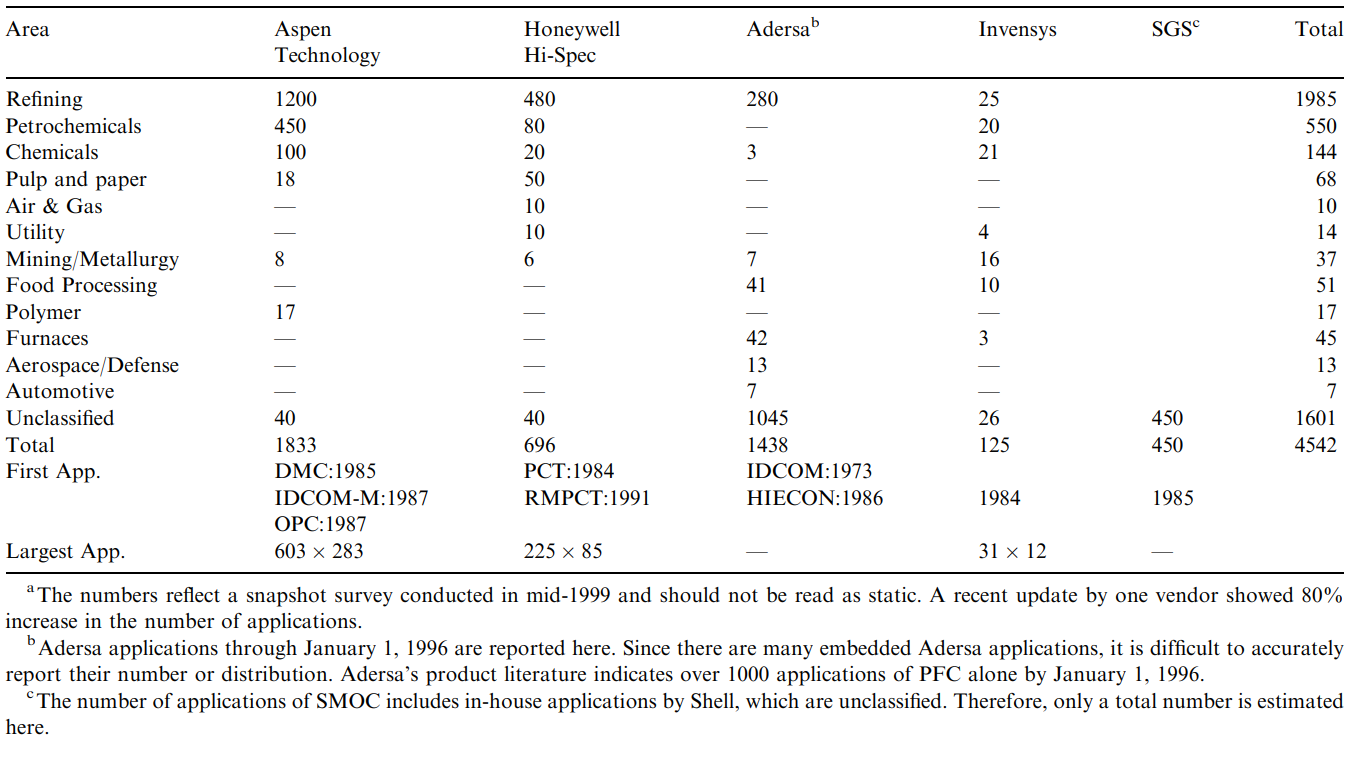
\includegraphics[scale=0.28]{mpc_usage_table}
	\caption{Summary of linear MPC applications by areas}
	\label{mpc_usage_table}
\end{table}

In \cite{qin2003survey} is presented an overview of commercially available model predictive control technology, both linear and
nonlinear. The table \ref{mpc_usage_table} from that work shows the applications of MPC logic by area. Such a diffuse usage of this control logic collocate MPC as the second most used control methodology after PID. In the last decades MPC has been investigated in may fields as Process control (linear or nonlinear MPC), Automotive (Explicit, Hybrid MPC), Aerospace(LTV MPC), ICT(distributed/decentralized MPC), Energy or Finance (stochastic MPC).
As most of the drawbacks are related to the model identification or optimization algorithms capability, fields in which research is working nowdays, MPC is still of high importance for research and industry.
In this section basic concepts of Model Predictive Control will be presented in order to understand more in detail what we developed. More details in MPC theory can be found in \cite{camacho2013model}

\subsection{Basic Concepts}

As mentioned before Model Predictive Control use the model of the system and the definition a customized cost function in order to set and solve an optimization problem to find the correct control inputs to perform a specific control task.
A diagram of how MPC basic architecture is schematized below: \\
 
\begin{figure}[h!]
	\centering
	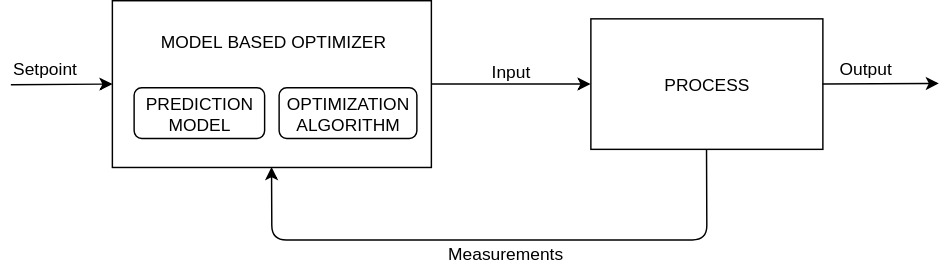
\includegraphics[scale=0.4]{MPC_base_diagram}
	\caption{MPC basic architecture scheme}
	\label{mpc_base_diagram}
\end{figure}
The model based optimizer (usually a computer) use optimization algorithms in accordance with the model of the system and given measures to minimize the cost function which is generally dependent on the error with respect to the given setpoint. Generally other constraints can be added to the problem in order for example to keep the states variables within feasible ranges. The output of the computation is then the input of the real process to be controlled. In  practice the solution of the problem usually has two main limitation:

\begin{itemize}
\item Model of the process: the nature of the MPC is based on the possibility to forecast the future output of the system by means of a model. Because of that, to have a reliable prediction, we need the system model to be accurate.

\item Optimization algoritm: as mentioned before, the more the system is complex and constraints are added to the problem, the more the problem will be computationally heavy. A proper optimization algoritm needs to be choose in accordance with the application of the controller.
  
\end{itemize}
Any controller belonging to MPC family is usually amenable to the following methodology:
\begin{figure}[h!]
	\centering
	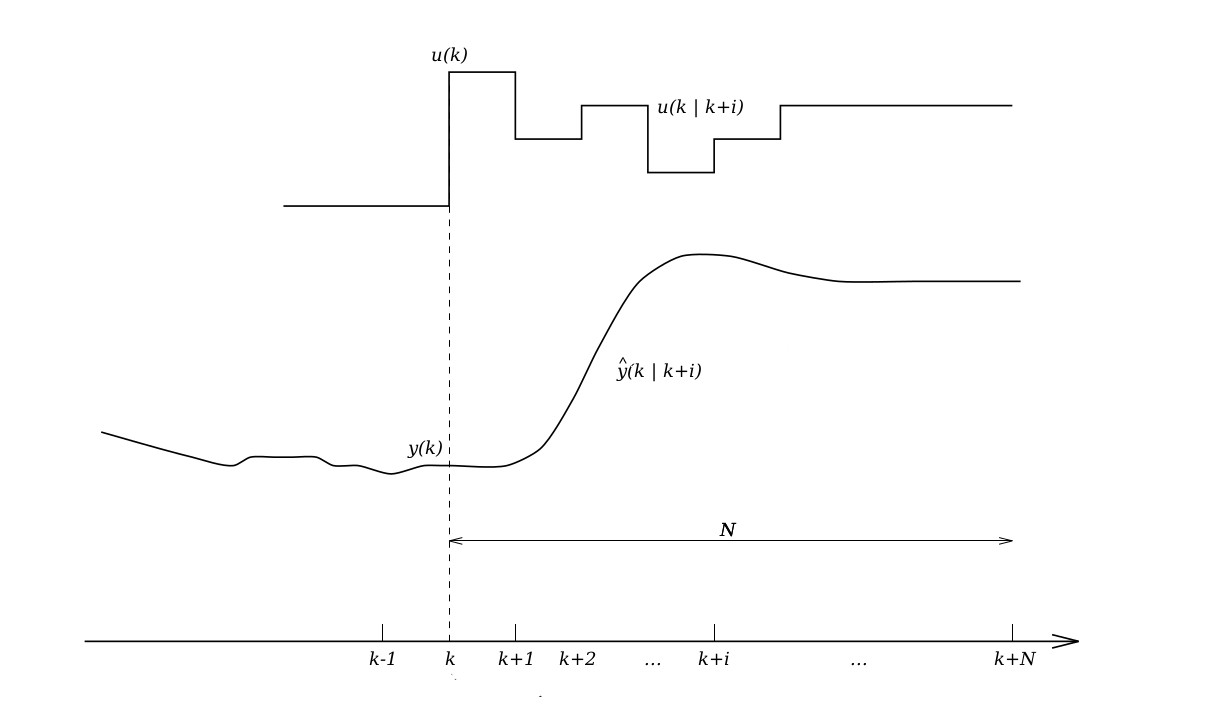
\includegraphics[scale=0.32]{mpc_horizon_base_scheme}
	\caption{MPC strategy}
	\label{mpc_horizon_base_scheme}
\end{figure}

\begin{enumerate}
\item Future outputs defined on a prediction horizon $N$ as $\hat{y}(k|k+i)$ for $i=1\ ...\ N-1$ are predicted starting from past inputs and outputs as a function of the future control actions $u(k|k+i)$, $i=0\ ...\ N-1$.
\item The future control signal set is calculeted optimizing a given cost function to keep the predicted future output as close as possible to the given reference trajectory $y_d(k+i)$. The objective function is generally defined as a quadratic fuction with respect to this reference trajectory. Control effort term is also usually added to the cost in most cases. If the system is linear and the cost function is quadratic with respect to the error then an explicit solution can be found, otherwise merical methods have to be used instead.
\item The computed control action $u(k|k)$ is applied to the process then another optimization problem is set based on new measures in order to find $u(k+1|k+1)$ that will be in principle different from $u(k|k+1)$. 
\end{enumerate}
The sequence above repeats continuously following the so called Reciding Horizon principle. In order to be implemented, the model based optimizer, is designed following this scheme: \\
\begin{figure}[h!]
	\centering
	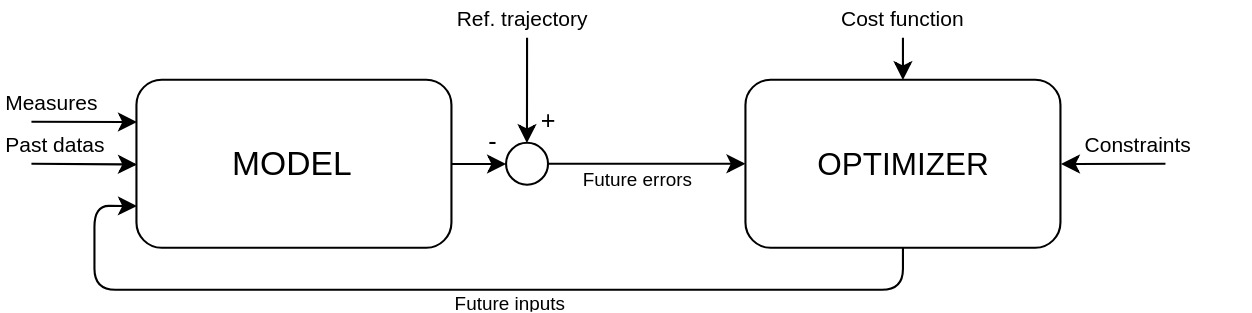
\includegraphics[scale=0.32]{scheme_model_based_opt}
	\caption{Model based optimizer}
	\label{scheme_model_based_opt}
\end{figure}
\\
The definition of prediction model can be done in several ways like inpulse response, step response, transfer function, state space and more complex representation like neural networks for nonlinear systems. We will refer to the state space representation for the prediction model as it is easy to implement and to integrate.

Let's define the discrete linear time invariant (LTI) model of the process in state space form as:

\begin{equation} \label{system_evolution}
	\begin{split}
		\begin{cases}
			x_{k+1}&=Ax_k+Bu_k \\
			y_{k+1}&=Cx_k
		\end{cases}
	\end{split}
\end{equation}

where $x \in R^{n_x}$ is the state, $y \in R^{n_y}$ and $u \in R^m$ are respectively the output and the control action and $A$, $B$ and $C$ are the matrices of the system. The prediction of the output for this model is given then by:

\begin{equation}\label{system_prediction}
	\hat{y}(k\ |\ k+i)=C\hat{x}(k\ |\ k+i)=C\left[A^i x(k) + \sum_{j=1}^{i} A^{j-1}Bu(k\ |\ k+i-j)\right]
\end{equation}

which can be defined in matrix form as: 
\begin{equation}
\begin{split}
	\left[ \begin{matrix} \hat{x}_k(1) \\ \hat{x}_k(2) \\ \vdots \\ \hat{x}_k(N) \end{matrix} \right] = \underbrace{\left[ \begin{matrix}
	CB		 & 	0	    &	\dots	&	0 		\\
	CAB		 & 	CB	    &	\dots	&	0 		\\
	\vdots	 &  \vdots  &	\ddots	&	\vdots	\\
	CA^{N-1}B & CA^{N-2}B &   \dots   &	CB			
	\end{matrix}\right]}_{\bar{H}}\left[ \begin{matrix} u_k(0) \\ u_k(1) \\ \vdots \\ u_k(N) \end{matrix} \right]+ \underbrace{\left[ \begin{matrix} CA \\ CA^2 \\ \vdots \\ CA^N \end{matrix} \right]}_{\bar{T}}
	\end{split}	
\end{equation}

The definition of the cost function has a strong influence on stability proof as well as the convergence of numerical optimization methods. A preferrable choice is to consider a positive definite function of the error with respect to the reference trajecotry. As the problem can be easily moved a zero-reference problem we will refere to that case. For simplicity of notation we will refer to $\hat{y}(k\ |\ k+i)$ as $\hat{y}_{k|i}$
\begin{equation} \label{costfunction}
	\begin{split}
		J(x_{k|0},\textbf{u}_k) = \sum_{i=0}^{N-1} \left[\hat{y}_{k|i}^T Q \hat{y}_{k|i} + u_{k|i}^TRu_{k|i} \right] + \hat{y}_{k|N}^T P \hat{y}_{k|N}
	\end{split}	
\end{equation}

where $\textbf{u} \in R^{mXN}$ with $\textbf{u} = [u_{k|1}\ u_{k|2}\ ...\ u_{k|N-1}]$ is the control action that has to be found for the predicted horizon. R, Q and P are positive definite weight matrices. Let's write the cost function in matrix form: 

\begin{equation*}
\begin{split}
		J(x_{k|0},\textbf{u})&=x_{k|0}^T Q x_{k|0} + 
		\left[ \begin{matrix} \hat{x}_{k|1} \\ x_{k|2} \\ \vdots \\ \hat{x}_{k|N} 		\end{matrix} \right]^T \underbrace{\left[ \begin{matrix} 
Q	 		&		 0	  	&  	0	  &  \dots  &  0 \\ 
0 			&  	 Q 	  	& 		0 	  &  \dots  &  0 \\
\vdots  	& 	  \vdots  	&   \ddots   &  \vdots &  0 \\
0 			& 	  \dots  	&      0     &      Q  &  0 \\
0			& 		 0 		&	  \dots   &      0  &  Q
\end{matrix} \right]}_{\bar{Q}}
\left[ \begin{matrix} \hat{x}_{k|1} \\ x_{k|2} \\ \vdots \\ \hat{x}_{k|N} \end{matrix} \right] +  \\ 
&+\left[ \begin{matrix} u_{k|0} \\ u_{k|1} \\ \vdots \\ u_{k|N-1} 		\end{matrix} \right]^T \underbrace{\left[ \begin{matrix} 
R	 		&		 0	  	&     \dots   &  0 \\ 
0 			&  	     R 	  	&     \dots	  &  0 \\
\vdots  	& 	  \vdots  	&    \ddots   &  \vdots \\
0			& 	  \dots     &        0    &  R
\end{matrix} \right]}_{\bar{R}}
\left[ \begin{matrix} u_{k|0} \\ u_{k|1} \\ \vdots \\ u_{k|N-1}  \end{matrix} \right] 
\end{split}
\end{equation*}

Substituting the \ref{system_prediction} we obtain:

\begin{equation}\label{costfunction_expr}
\begin{split} 
 J(x_{k|0},\textbf{u}_k)&=x_{k|0}^T Q x_{k|0} + (\bar{S}\textbf{u}_k+\bar{T}x_{k|0})^T\bar{Q}(\bar{S}\textbf{u}_k+\bar{T}x_{k|0}) + \textbf{u}_k^T\bar{R}\textbf{u}_k \\ 
 &= \frac{1}{2}\textbf{u}_k^T \underbrace{2(\bar{R}+\bar{S}^T\bar{Q}\bar{S})}_{H}\textbf{u}_k + x_{k|0}^T\underbrace{2\bar{T}^T\bar{Q}\bar{S}}_{F}\textbf{u}_k+\frac{1}{2}x_{k|0}\underbrace{2(Q+\bar{T}^T\bar{Q}\bar{T})}_{Y}x_{k|0} \\
 &=\frac{1}{2}\textbf{u}_k^TH\textbf{u}_k+x_{k|0}F\textbf{u}_k+\frac{1}{2}x_{k|0}Yx_{k|0}
 \end{split}
\end{equation}
Once we have express the cost as a function of the measured initial state $x_k(0)$ and the future control action we can perform the optimization by zeroing the gradient:
\begin{equation}
	\nabla_{\textbf{u}_k}J(x_{k|0},\textbf{u}_k)=H\textbf{u}_k+F^Tx_{k|0}=0
\end{equation}
\label{grad_obj_fun}
$\textbf{u}_k$ is then derived inverting the \ref{grad_obj_fun}:
\begin{equation*}\label{MPC_control_law}
	\textbf{u}_k= \left[
	\begin{matrix}
			u_{k|0} \\ u_{k|1} \\ u_{k|2} \\ \vdots \\ u_{k|N-1}
	\end{matrix}\right] = -H^{-1}F^Tx_{k|0}
\end{equation*} 

The contorl law generated that can be derivated is then:
\begin{equation}
u(t)=-\left[\ I\ 0\ \dots\  0\ \right]H^{-1}Fx(t)\triangleq Kx(t)
\end{equation}
The same result can be obtained from DARE (discrete-time Algebraic Riccati Equation) as done in \cite{magni2006complementi}.
By means of this result it is possible to implement the MPC with a simple feedback loop. Since it is possible, the derivation of \ref{MPC_control_law} is done offline in this case, the online controller will then be fast given that the computational effort depend almost only on the inversion of $H$. 
Anyway the assuptions of Linear and time invariant system are considerably strong, many of practical systems present nonlinearities an time varying relationship. Because of that, different ways to minimize the \ref{costfunction_expr} have to be found.
Usually what is done in practice is to use algorithms to perform numerical optimization to find an approximation of the optimal solution. The main issue in the solution of the optimization problem is related to the well-definiteness of the problem. Indeed the correct choice of objective function form has to be done. usually the quadratic form allows to define convex problems in order to guarantee the unicity of the solution.

\subsection{Constraints}

In order to take into account feasibility sets and to gurantee stability, constraints are usually added to the optimization problem that becomes: 

\begin{equation} \label{MPC_problem_constrained}
\begin{split}
		&\qquad min_{\textbf{u}_k}\ J(x_{k|0},\textbf{u}_k) \\
		\textnormal{where}\ \  
		 J(x_{k|0},\textbf{u}_k) &= \sum_{i=0}^{N-1} \left[\hat{y}_{k|i}^T Q \hat{y}_{k|i} + u_{k|i}^TRu_{k|i} \right] + \hat{y}_{k|N}^T P \hat{y}_{k|N} \\
		\textnormal{respecting}\ &  	
		\begin{cases}
			\hat{x}_{k+1}&=A\hat{x}_k+Bu_k \\
			\hat{y}_{k+1}&=C\hat{x}_k
		\end{cases} \\
		\textnormal{s.t.}\qquad
		&\ \ \ \ 0 \leq f(x)\leq 0 \\
		&\ \ \ \ 0 \leq g(u)\leq 0 \\
	\end{split}	
\end{equation}

This notation allows us to introduce both equality and inequality constraints. In paractice the constraints are divided into: 
\begin{itemize}
 \item \textbf{Input constraints}: generally represent philical limitation for the control $\textbf{u}_k$ and are defined as "hard" constraints.
 	\item \textbf{State/Output constraints}: usually come from rescrictions into the operational space, they can both be "soft" or "hard".
\end{itemize} 

Hard constraints on the state or on the output gives generally complication in the implementation but soft constraints have to be defined properly according to the application. Moreover constraints allows a resonable control action to be generated when measured or estimated states moves outside the feasible sets. Given this outline, many are the possible constraints definition: Band Constraints, Overshoot Constraints, Monotonic Behaviour, Nonminimum Phase Behaviour, Actuator Nonlinearities, Terminal State Equality Constraints, Terminal Set Constraints and more. Given that it is possible to define different constraints we will refer to terminal state equality constraint as it will be useful for the stability proof later on. \\
The terminal state constraint is basically defined as: 

\begin{equation}
\hat{y}_{k|N}=C\left[A^i x_{k|0} + \sum_{j=1}^{i} A^{j-1}Bu_{k|k+N-j}\right]=\bar{y}_N
\end{equation}
that can be rewritten following the form in \ref{MPC_problem_constrained}: 
\begin{equation}
0 \leq \hat{y}_{k|N}-\bar{y}_N \leq 0
\end{equation} 

\subsection{Stability and Feasibility}

In this section stability and feasibility of MPC are investigated in order to give a clear understanding of what done to proof stability of the MPC we developed. To assess feasibility we need to investigate and proff is the problem have a solution and then to proof recursive feasibility, so the system accept a solution $\forall\  t>0$. As well as feasibility, stability has to be proof in order to have convergence of the performed trajecotry. We will refer to a regulation problem, so the set point will be defined as the origin.
The set $X_{k}$ of initial states $x_{k|0}$ defined for any instant $k$ that ensure feasibility for the MPC problem \ref{MPC_problem_constrained} is defined as:

\begin{equation}
	\begin{split}
		X_{k}=\lbrace\ x_{k|0}\in\mathbb{R}^n\ |\ \exists\  (u_{k|0}, \dots , u_{k|N-1})\ \textnormal{s.t.}\ x_{k|i} \in X, u_{k|i} \in U,\ &  \\ 
		\forall\  i=0,\dots,N-1,\ x_{k|N} \in X_f\ \rbrace& \\ 
	\end{split}
\end{equation}
where $U$ is the region of the control action, $X_f$ is the region of terminal states and $x_{k|i+1}$ is propagated following the \ref{system_evolution}
 The feasible and unfeasible points in a regulation problem can be visualized on a graph (see \ref{feasibility_image1}) and a region of feasible points can be defined (see \ref{feasibility_region})

 \begin{figure}%
\centering
\subfigure[Feasibility points]{%
\label{feasibility_image1}%
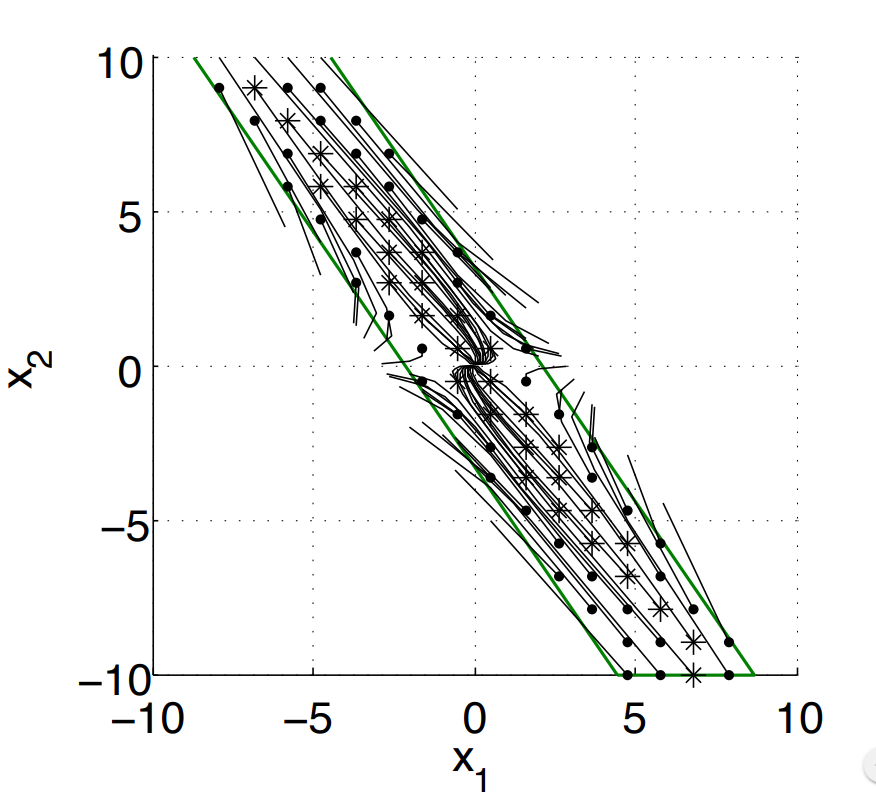
\includegraphics[scale=0.2]{feasibility_image1}}%
\qquad
\subfigure[Feasibility region]{%
\label{feasibility_region}%
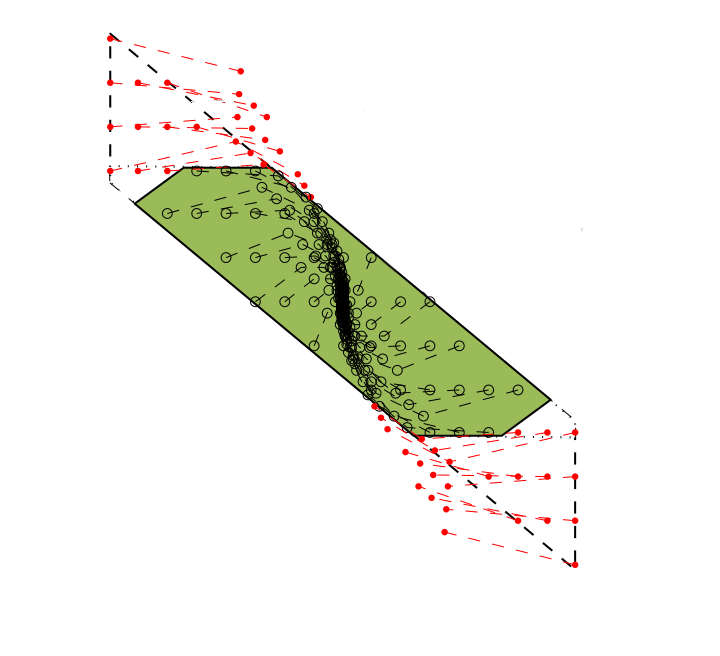
\includegraphics[scale=0.25]{feasibility_region}}%
\caption{Feasibility set}
\end{figure}

 Feasibility of a point does not guarantee the feasibility of the following inputs generated by the control action. Because of that Recursive feasibility has to be assessed. That means to show that:
 \begin{equation}
 \begin{split}
  &\ \ \ \ \ \ \ \ \ \forall\ k\ \exists\  \textbf{u}_k\in U\  \textnormal{s.t. } \\ 
  \textnormal{given } &x_{k|0} \in X, \  x_{k|i} \in X\  \forall\ i = 1,\  \dots\ , N-1   
 \end{split}
 \end{equation}
\begin{figure}[h!]
	\centering
	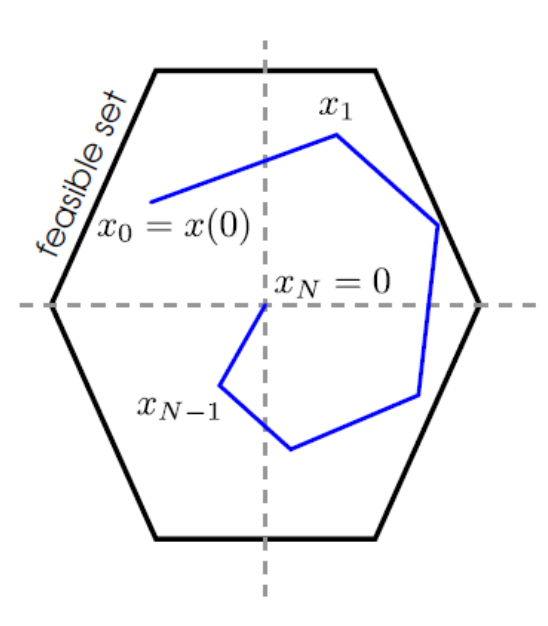
\includegraphics[scale=0.27]{feasible_image2}
	\caption{Recursive feasibility}
	\label{feasible_image2}
\end{figure}

While feasibility proof is straightforward because it is only affected by outputs hard constraints, stability is difficult to assess in some cases.
Stability is a complex function of $N, Q, R, P, U$ and admissible outputs of the system.
Usually the stability proof of the MPC is verified imposing terminal constraints and weigths on the terminal state. There are many well studied stability proofs for MPC problems:

\begin{itemize}
\item Infinite horizon MPC (N = $\inf$) with no additional constraints
\item Terminal point constraints ($x_{k|N}=0$)
\item Relaxed terminal constraints ($x_{k|N} \in X_f $)
\end{itemize}

The equilibrium point of a controlled system is said to be Lyapunof stable in $X$ if $\forall k \in \mathbb{N}$
\begin{equation}
\begin{split}
\forall&\ \epsilon > 0, \exists\ \delta(\epsilon) >0 \textnormal{ such that } \forall x_{k|0} \in X : \\
&||x_{k|0}|| \leq \delta(\epsilon) \implies ||x_{k|i}|| < \epsilon \forall\ i \in \mathbb{N}
\end{split}
\end{equation}

Stability proof is generally made by showing that the cost function to be minimized is a Lyapunov Function and admits an equilibrium point in the origin (regulation problem). The if $J$ is a Lyapunov function, the equilibrium point is stable with region of attraction $X$.

A function $V:X\rightarrow\ \mathbb{R}_+$ is a Lyapunov function if $\forall\ x \in\ X$:
\begin{equation} \label{Lyap_func}
\begin{split}
	V(x)>0 \rightarrow& \forall\ x \neq 0 \\
	V(0)=&\ 0 \\
	V(x_{k+1})-V(&x_{k}) \leq 0
\end{split}
\end{equation}

In order to guarantee convergence, asymptotic stability in $X$ of the equilibrium point has also to be verified. Hence it's needed to verify that it is Lyapunov stable and attractive in $X$ ( $\lim_{k \to \infty}||x_k||=0\ \forall\ x\ \in\ X$ ). 
That can be verified by extending the \ref{Lyap_func} asking: 
\begin{equation}
	V(x_{k+1})-V(x_{k}) < 0
\end{equation} 
\\ 
\\
Now let's consider for simplicity the cas in which $C=I$ so the system in \ref{system_evolution}becomes:
\begin{equation*}
x_{k+1}=Ax_k+Bu_k
\end{equation*}

We will assess stability by means of terminal constraints imposition (i.e. $x_{k|N}=0$) considering the quadratic cost function in \ref{costfunction} with  $J(x_{k|0},\textbf{u}_k)=J_k(x_0,\textbf{u})$
\begin{equation}
\begin{split}
J_k(x_0,\textbf{u}) &= \sum_{i=0}^{N-1} \underbrace{\left[x_{k|i}^T Q x_{k|i} + u_{k|i}^TRu_{k|i} \right]}_{q(x_i,u_i)} +\ \underbrace{x_{k|N}^T P x_{k|N}}_{p(x_N)} \\
\textnormal{and}\ \  x_n&=0
\end{split}
\end{equation}

Recursive feasibility has first to be verified:
Assuming the feasibility of the point $x_0$ and defining $[u_0^*,\ u_1^*,\ \dots,\ u_{N-1}^*]$ the optimal control sequence computed minimizing $J_0(x_0,\textbf{u})$, following the MPC strategy we apply $u_0^*$. The evolution of the system will then be $x_1=Ax_0+Bu_0^*$.
Now at instant $k=1$ the control sequence $[u_0^*,\ u_1^*,\ \dots,\ u_{N-1}^*,\ 0]$ is feasible because applying a null control input and given that $x_N=0$ the resulting final state is $x_N+1=0$. This implies that, in presence of end point constraints, the recursive feasibility is verified assuming $x_0$ feasible.

Once feasibility has been assessed, stability has to be investigated by checking if $J$ is a Lyapunov function. So, since we are interested in asymptotic stability, we need to verify;

\begin{equation}
J_0^*(x_1)<J_0^*(x_0)\ \ \ \forall x_0 \neq 0
\end{equation}

Follows that:
\begin{equation}
	\begin{split}
		&J_0^*(x_0)= \underset{=0}{\cancel{p(x_N)}}+\sum_{i=0}^{N-1} q(x_i,u_i^*) \\
		&J_0^*(x_1) \leq \tilde{J}_0(x_1)=\sum_{i=1}^{N}q(x_i,u_i^*) \\
		 = \sum_{i=1}^{N-1}&q(x_1,u_i^*)-q(x_0,u_0^*)+q(x_N,u_N) \\
		 &\ =\  J_0^*(x_0)-q(x_0,u_0^*)+\underset{=0}{\cancel{q(0,0)}} \\
	\end{split}
\end{equation}

Then what can be said is that:
\begin{equation}
	J_0^*(x_1)-J_0^*(x_0)\leq \tilde{J}_0^*(x_1) - J_0^*(x_0) \leq -q(x_0,u_0^*) \leq 0
\end{equation}

Hence, $J*(x)$ is a Lyapunov function, so the point $x_N=0$ is an asymptotically stable point for the control law. This concept can be generalized for different kind of problem. Anyway, as mentioned before, there are other ways to verify stability which depends on how is the problem defined. Summarizing, terminal constraints imposition provides a sufficient condition for stability in practice what is done is to enlarge the control horizon and sampling since the system perform stability. 

\subsection{NMPC}

The basic concepts of MPC have been investigated so far considering linear systems. In general, most of the systems are nonlinear, but even in presence of linearities the use of linear controllers like linear MPC is widely diffuse. There are two many reasons for that: on one hand approximating the model of the system as linear gives good results when it moves in the neighberhood of a stationary point, on the other hand the system parameter estimation for linear systems based on measurements is relatively easy. Futhermore, the minimization of a quadratic cost function in presence of a linear system (i.e. quadratic programming) has been well studied and many commercial products ae available (see \ref{mpc_usage_table}). Moreover, in fast sampling time applications the usage of a linear model provides faster solving time in order to keep the time used to solve the optimization problem lower than the sampling time of the system.
Nevertheless there are systems for which the number of dynamic response of the resulting linear controller is unacceptable, expecially in systems highly nonlinear. The solution adopted using nonlinear MPC is generally not suitable, for example, in applications where the dynamic system parameters may change over time. In those cases the adoption of nonlinear models is required. 
There is nothing in the theory overviewed in the previous section that prevent the usage of a nonlinear system, therfore the extension of what has been done to nonlinear models is straightforward, at least conceptually. However there are many problems that rises from that:

\begin{itemize}
\item The optimization problem becomes non-convex and because of that, to find a solution become not trivial. Local minima may occur influencing performances and stability.
\item The study of stability and robustness becomes more complex and is still an open field in research.
\item The computational time becomes a variable that has to be taken into account expecially for high speed systems.
\item The identification techniques in presence of nonlinear models are still an open field and model representation through first principles is not always feasible. New thecniques like Neural Networks or deep learning are being studied.
\end{itemize} 
If we con sinder as an example the nonlinear system:

\begin{equation}
y_{k+1}=0.9y_k+u_k^{\frac{1}{4}}
\end{equation}

the \ref{linearvsnl} shows the response when controlled with linear MPC approximating the system with $y_{k+1} = 0.9y_k+u_k$ or nonlinear MPC and we can see the response of the linear model based controller oscillates for the first set point values while the nonlinear model based is quite good. 


\begin{figure}[h!]
	\centering
	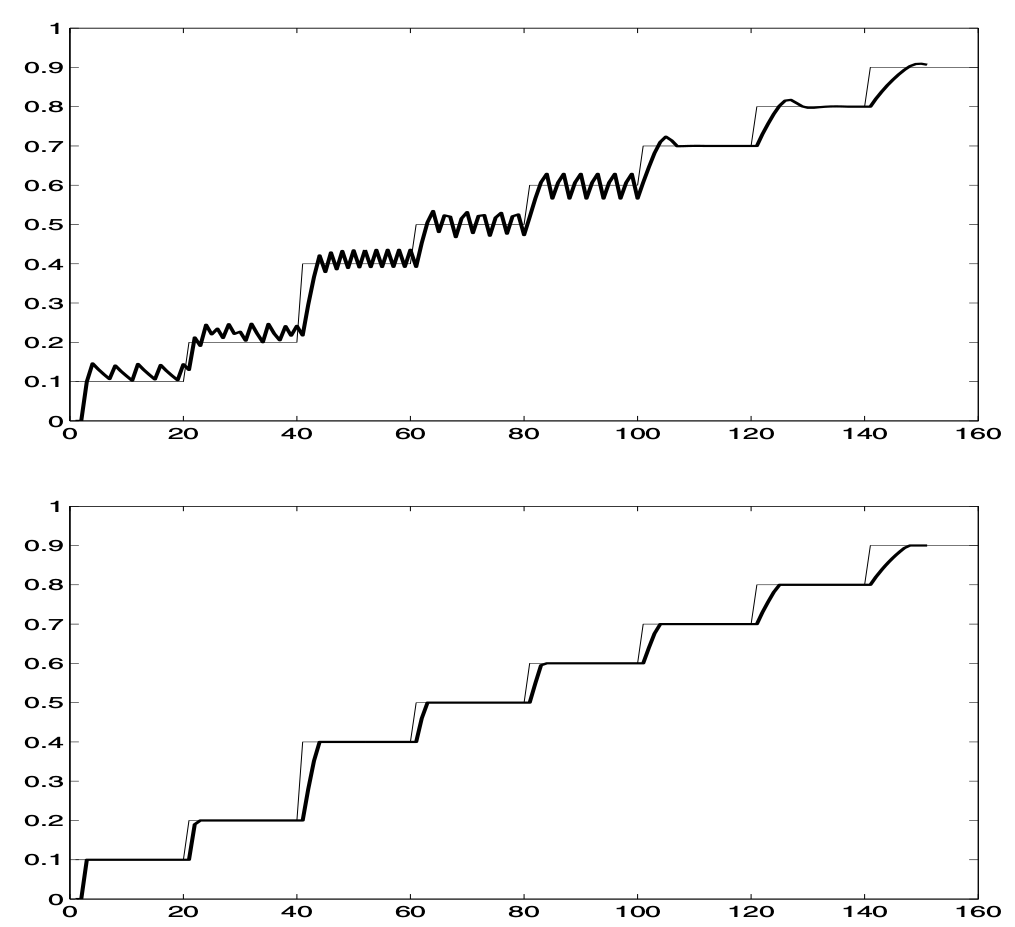
\includegraphics[scale=0.25]{linearvsnl}
	\caption{Linear vs. Nonlinear MPC}
	\label{linearvsnl}
\end{figure}


In general, since state space models are the most used and can be easily extended to consider nonlinearities, instead of the system in \ref{system_evolution}, we will consider:

\begin{equation}
\begin{split}
		\begin{cases}
			x_{k+1}&=f(x_k,u_k) \\
			y_{k+1}&=g(x_k)
		\end{cases}
	\end{split}
\end{equation} 

Now, given that $x_k$ is the state vector we can se that this representation allows us to represent both single variable and multi variable systems.
s rise to a lot of
Even if model parameters identification is an open issue for nonlinear systems, this is not the only difficulty related to nonlinear MPC. The increase of omputational time required and reliability of the solution have to be taken into account when dealing with online applications of NMPC. 
The nonlinear problems (NLP) is usually solved using Sequential Quadratic Programming
(SQP) techniques which are axtension of Newton-type methods for converging the solution of the KKT conditions of the given problem (see \cite{skkt}). The main challange in solving the problem is to guarantee convergence even in presence of ill conditioning and extreme nonlinearities.
In general if the time given to solve the NLP is not sufficient at one step, the last iteration $u_k$, which satisfies the local linear approximation to the constraints, is sent to the system, although it may violate the original constraints. Many approaches have been developed in the years to overcome the difficulties in solving NLP online dealing with suboptimal solutions and fast convergence. Since now we reviewd basic concepts of MPC logic in order to give an overview of what MPC is based on. Note that what showed can be easily extended for LTV systems since the time dependence of the parameters doesn't affect the cost function definition neither the stability proof.
\chapter{Mobile Manipulators Control Problem}
\label{chapter4}
We have seen that Mobile Manipulators are systems where locomotion and manipulation tasks are held simultaneously. The coordination of this two tasks is not trivial since the mobile platform combined with the manipulator is a redundant system. So, the same point in workspace can be reached moving the mobile base, or moving the manipulator, or with a combined motion of the two. In addition to this kinematic issue, also the dynamic interaction between mobile base and manipulator should be taken into account in a control logic. \\
In literature the control of mobile manipulators mainly followed two strategies. The first approach is the separate control of the mobile base and of the manipulator arm, considering then their interaction. With this approach is possible to simply solve the kinematic redundancy of the system. A reference for this approach can be \cite{liulewis} or \cite{chung1998interaction}. The second approach is the coordination of the motion of the base and the manipulator through the control of the whole integrated redundant system. 
We will split this chapter in the description of the control of the mobile base, followed in a seceond section by the problem of the integration of the manipulator in the control.
\section{Control of Mobile Robots}
Facing the control of the mobile base it is needed to deal with a nonholonomic system, which is nonlinear, as it has been written before.
Usually for the control of the motion of the mobile base the kinematic model is used applying as inputs to the system the commands for the longitudinal velocity $v$ and the steering velocity $\omega$. In this way it is possible to control directly the generalized velocities of the base, i.e. $\dot{x},\dot{y},\dot{\theta}$.
It would be certainly possible to use a dynamic based control of the motion through torques commands to the wheels of the base, but in most mobile robots, in particular in the one we used, the dynamic perturbation is very small, or it can be canceled through a proper state feedback. Moreover it is possible to command the mobile robot only via velocity commands.
The control of the mobile base can be implemented in two ways: regulation, i.e. driving the robot to a constant position and/or orientation, and trajectory tracking, i.e. forcing the robot to follow a time-varying reference trajectory.
\subsection{Regulation}
The regulation problem can be addressed in two ways.
\subsubsection{Cartesian Regulation}
\begin{figure}[h!]
	\centering
	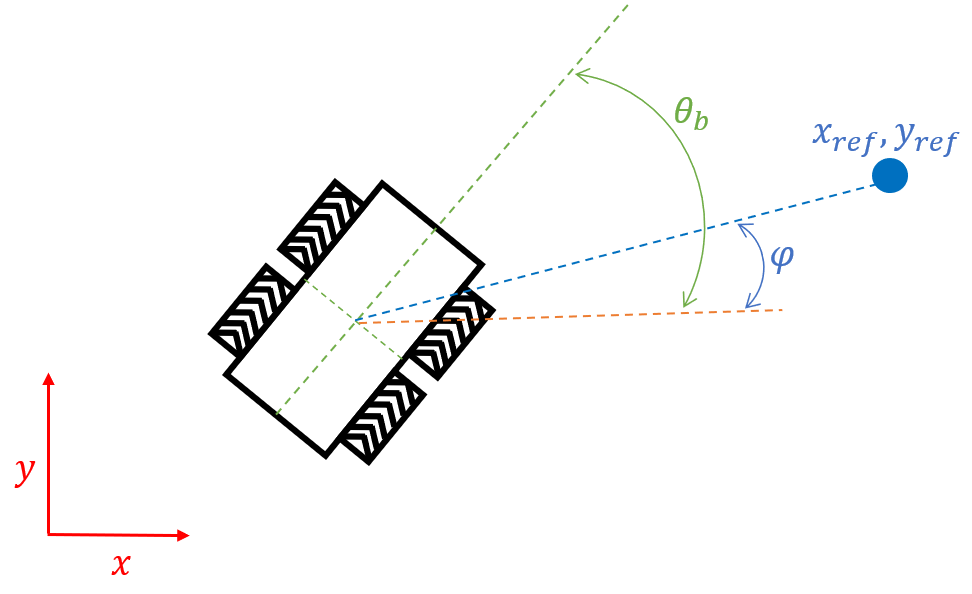
\includegraphics[scale=0.8]{cartesian_regulation}
	\caption{Cartesian Regulation problem}
	\label{cartregulation} 
\end{figure}
The robot (a unicycle) has to reach a point whose coordinates $(x_{ref},y_{ref})$ are defined in the Cartesian space. In this problem there is no need to control also the orientation of the robot. 
In literature several control laws have been proposed. Among others \cite{siciliano} reports: defining the Cartesian error $\mathbf{e}_P=(x_{ref}-x,y_{ref}-y)=(e_{P_x},e_{P_y})$ the control inputs can be obtained as
\begin{align}
	v &= k_1(e_{P_x}\cos\theta+e_{P_y}\sin\theta)\\
	\omega &= k_2\left(\text{Atan2}\left(e_{P_y},e_{P_x}\right)-\theta-\pi\right)
\end{align}
where $k_1$ and $k_2$ are positive constants. 
As \cite{siciliano} too says, these commands can be directly interpreted, because $v$ is proportional to the Cartesian error, driving the robot to $\mathbf{e}_P=0$, while the $\omega$ is steering the robot in the direction pointing to $(x_{ref},y_{ref})$, i.e. $\omega$ is proportional to the difference $\theta-\varphi$, where $\varphi$ is $\text{Atan2}\left(e_{P_y},e_{P_x}\right)$.
\subsubsection{Posture Regulation}
The robot has to get to a certain configuration, i.e. Cartesian position and orientation. 
Also in this case, the literature is full of control laws for this kind of problem. We report the control law found in \cite{dixon} and in \cite{samson}.
Defining, for a practical advantage, the transformation:
\begin{equation} \label{trackingerrortransformation}
 	\mathbf{e}=
 	\left[\begin{matrix}
		e_1\\e_2\\e_3
	\end{matrix}\right] = 
	\left[\begin{matrix}
		\cos\theta & \sin\theta & 0 \\
		-\sin\theta & \cos\theta & 0 \\
		0 & 0 & 1
	\end{matrix}\right]
	\left[\begin{matrix}
	x_{ref}-x\\y_{ref}-y\\\theta_{ref}-\theta
	\end{matrix}\right]
\end{equation}
Which are the errors in a local frame of the mobile robot, where $e_1$ is the error in the longitudinal direction and $e_2$ is the error in the transversal direction.\\ Deriving the above equation taking into account the kinematic relation \ref{G}:
\begin{equation}
	\left[\begin{matrix}
		\dot{e}_1\\\dot{e}_2\\\dot{e}_3
	\end{matrix}\right] = 
	\left[\begin{matrix}
		-v+\omega e_2\\-\omega e_1\\\omega
	\end{matrix}\right]
\end{equation}
The proposed control law for $v$ and $\omega$ is:
\begin{equation}
	\left[\begin{matrix}
	v\\\omega
	\end{matrix}\right] = 
	\left[\begin{matrix}
	-k_1e_1\\-k_2e_3+e_2^2\sin(t)
	\end{matrix}\right]
\end{equation}
where $k_1$ and $k_2$ are positive constants. So the closed-loop dynamics becomes:
\begin{equation}
	\left[\begin{matrix}
	\dot{e}_1\\\dot{e}_2\\\dot{e}_3
	\end{matrix}\right] = 
	\left[\begin{matrix}
	k_1e_1+\omega e_2\\-\omega e_1\\-k_2e_3+e_2^2\sin(t)
	\end{matrix}\right]
\end{equation}
For the stability proof of this control law we refer to \cite{dixon}.
\subsection{Trajectory Tracking}
A \textit{trajectory} is a path, i.e. the locus of points which the robot has to follow in the execution of the assigned motion, over which a timing law has been assigned. \\
So a trajectory can be represented as the time history $x_d(t),y_d(t)$, but in the case of a mobile robot the trajectory has also to be admissible, because it has to respect the nonholonomy of the system, i.e. it must satisfy the relation \ref{A}:
\begin{equation} \label{admissibletrajectory}
	\begin{split}
		\dot{x}_d &= v_d\cos\theta_d\\
		\dot{y}_d &= v_d\sin\theta_d\\
		\dot{\theta}_d&=\omega_d
	\end{split}
\end{equation}
Usually reference trajectories for mobile robots are being computed by planning algorithms so that \ref{admissibletrajectory} is satisfied, but they give in output just the Cartesian coordinates' time history. The orientation reference trajecory can be computed as:
\begin{equation}
	\theta_d(t)=\text{Atan2}(\dot{x}_d(t),\dot{x}_d(t)) 
\end{equation}
 And also the resulting reference control inputs can be calculated.
 \begin{align}
 	v_d(t)&=\sqrt{\dot{x}_d^2(t)+\dot{y}_d^2(t)}\\
 	\omega_d(t)&=\frac{\ddot{y}_d(t)\dot{x}_d(t)-\ddot{x}_d(t)\dot{y}_d(t)}{\dot{x}^2_d(t)+\dot{y}^2_d(t)}
 \end{align}
 To quantify the tracking control objective the tracking error vector $\mathbf{e}$ is defined as before (\ref{trackingerrortransformation}), but in trajectory tracking problems the derivative of $\mathbf{e}$ is different than in regulation problems because the derivative of the reference trajectory is no more null.
 \begin{equation}
 	\left[\begin{matrix}
 		\dot{e}_1\\\dot{e}_2\\\dot{e}_3
 	\end{matrix}\right] = 
 	\left[\begin{matrix}
	 	v_{ref}\cos e_3 - v+\omega e_2\\v_{ref}\sin e_3-\omega e_1\\\omega_{ref}-\omega
 	\end{matrix}\right]
 \end{equation}
 The tracking error dynamics is nonlinear, so the control of the system can be addressed with a nonlinear control or linearizing the system with a suitable transformation.
\subsubsection{Nonlinear Control}
A common used Nonlinear Control for trajectory tracking can be found in \cite{samsonCanudas},\cite{samson},\cite{dixon} and \cite{siciliano}, as follows:
\begin{equation}
	\left[\begin{matrix}
	v\\\omega
	\end{matrix}\right] = 
	\left[\begin{matrix}
	-k_1e_1+v_{ref}\cos e_3\\-v_{ref}\frac{\sin e_3}{e_3}-k_2e_3+\omega_{ref}
	\end{matrix}\right]
\end{equation}
Where $k_2$ is a positive constant and $k_1$ and $k_3$ are positive gains which depend on the values of $v_{ref}$ and $\omega_{ref}$. \\ So the closed-loop error dynamics becomes:
 \begin{equation}
	\left[\begin{matrix}
	\dot{e}_1\\\dot{e}_2\\\dot{e}_3
	\end{matrix}\right] = 
	\left[\begin{matrix}
	\omega e_2-k_1e_1\\v_{ref}\sin e_3-\omega e_1\\-v_{ref}\frac{\sin e_3}{e_3}-k_2e_3
	\end{matrix}\right]
\end{equation}
Also here, for the stability proof of this control law we refer to \cite{dixon}.
\subsubsection{Feedback Linearization}
Input/Output linearization is a commonly used way to face both regulation and trajectory tracking problems for mobile robots, but it has been seen that paradoxically it solves more easily trajectory tracking problems than regulation ones.
The idea of Feedback Linearization is to move the control problem to the trajectory of a point $P$ placed at a distance $\epsilon$ from the centre of the mobile robot in the direction of the longitudinal velocity.
Its coordinates are
\begin{equation}
	\begin{split}
		x_P&=x+\epsilon\cos\theta\\
		y_P&=y+\epsilon\sin\theta
	\end{split}
\end{equation}
Which differentiated are the velocities of $P$:
\begin{equation}
	\left[\begin{matrix}
		\dot{x}_P\\\dot{y}_P
	\end{matrix}\right]=\left[\begin{matrix}
		\dot{x}_P-\dot{\theta}\epsilon\sin\theta\\
		\dot{y}_P+\dot{\theta}\epsilon\cos\theta
	\end{matrix}\right]=\left[\begin{matrix}
	\cos\theta & -\epsilon\sin\theta\\
	\sin\theta & \epsilon\cos\theta
	\end{matrix}\right]\left[\begin{matrix}
	v\\\omega\end{matrix}\right]=T(\theta)\left[\begin{matrix}
	v\\\omega\end{matrix}\right]
\end{equation}
The determinant of matrix $T(\theta)$ is equal to $\epsilon$ and therefore always different from $0$ as long as $b=0$. Thence the inverted relation is:
\begin{equation} 
	\left[\begin{matrix}
		v\\\omega\end{matrix}\right]
	=\left[\begin{matrix}
		\cos\theta & \sin\theta\\
			-\frac{1}{\epsilon}\sin\theta & \frac{1}{\epsilon}\cos\theta
	\end{matrix}\right]\left[\begin{matrix}
		u_1\\u_2
	\end{matrix}\right] 
\end{equation}
Where $u_1$ and $u_2$ are the new linearized output of the controller. Indeed thanks to the feedback linearization, a simple linear model can be rewritten:
\begin{equation}
	\left[\begin{matrix}
		\dot{x}_P\\\dot{y}_P
	\end{matrix}\right]=\left[\begin{matrix}
		u_1\\u_2
	\end{matrix}\right]
\end{equation}
And so a very simple linear controller can be defined as in \cite{siciliano} without using a state error, but an output error:
\begin{equation}
	\begin{split}
		u_1&=\dot{x}_{P_{ref}}+k_1\left({x_P}_{ref}-x_P\right)\\
		u_2&=\dot{y}_{P_{ref}}+k_2\left({y_P}_{ref}-y_P\right)
	\end{split}
\end{equation}
Where $k_1$ and $k_2$ are positive gains. \\
It has to be noted that the orientation of the unicycle  $\theta$ is not controlled, but its time evolution due to the control inputs $u_1$ and $u_2$ can be modeled as:
\begin{equation}
 	\dot{\theta}=\frac{u_2\cos\theta-u_1\sin\theta}{\epsilon}
\end{equation}
Also a notation on the value of $\epsilon$ has to be added, because with smaller values of $\epsilon$ is possible to track more precisely a trajectory even if it involves curves with a small radius, but decreasing $\epsilon$, $T(\theta)$ tends to be singular, therefore leading to much higher values of $v$ and $\omega$.

\section{Control of Mobile Manipulators}
Although Mobile Manipulators are a known technology from decades, the control of these systems is still sparse. In literature many approaches have been proposed to face the kinematic redundancy of the Mobile Manipulator system. \\
A typical Mobile Manipulator consists of a nonholonomic base with 2 degrees of freedom (considering the nonholonomic constraint on the generalized velocities) and an arm which usually have 6 degrees of freedom, for a total of $n=8$; anyway, for vector $X_{ee}$ of the position and orientation of the end effector position has only $m=6$ components to be defined. The remaining $r=n-m=2$ redundant degrees of freedom can be exploited to solve the kinematic redundancy problem, mentioned in section \ref{dirinvkin}, satisfying a set of user-defined additional tasks. As explained in \cite{bayle},\cite{seraji1998},\cite{seraji1993} and \cite{mikschschroeder}, these additional tasks are described by a set of internal coordinates which defined as kinematic function of the coordinates $\xi=\left[x^T ; q^T\right]$
\begin{equation}\label{Phi}
	\Phi=g(\xi)
\end{equation}
These internal coordinates can have different physical meanings (like the distance between the wrist of the manipulator from the arm) or mathematical meanings (such as the projection of the gradient of an objecive function). There is not a fixed set of kinematic functions to pick, but the user can define those according to the task that has to be performed. A new extended vector $X_{ext}$ can be defined as:
\begin{equation}
	X_{ext}=\left[\begin{matrix}
	X_{ee} \\ \Phi
	\end{matrix}\right]
\end{equation}
The control problem now becomes a trajectory tracking of ${X_{ext}}_{ref}(t) =\left[\begin{matrix} {X_{ee}}_{ref}^T(t) \ ;\ \Phi_{ref}^T(t) \end{matrix}\right]$, where $ \Phi_{ref}(t)$ is defined by the relation \ref{Phi} over time.\\
The trajectory tracking problem usually consists in the optimization of an objective function $\varphi(q)$ defined with one or multiple properly weighted criteria, some of which are shown in \cite{multicriteria}. The most used optimization criteria are: 
\begin{itemize}
	\item The maximization of the manipulability of the system. See \cite{yamamoto}. A short description of what manipulability will follow.
	\item The minimization of the torque inputs. See \cite{chen1997dynamic}.
	\item The minimization of the deviation from the mid-range joints of the manipulator. See \cite{khatib1999}.
\end{itemize}
Clearly in addition to all these terms one is added for the minimization of the tracking error for all the vector $X_{ext}$.\\
It is not mandatory to extend the controlled vector adding internal coordinates in order to solve the kinematic redundancy problem. The additional tasks that the robot is asked to accomplish can be obtained adding a term to be minimized, e.g. the manipulability index, in the optimization problem. See for example \cite{bayle1} or \cite{bayle2} where the control is divided in two terms, one term that imposes the joint velocities  through the pseudo-inverse matrix of $J(q)$ and one term to maximize the manipulability of the system.\\
Exposing these methods we haven't had to specify wheter a kinematic or dynamic model is used, leaving the user the possibility to choose the more suitable one with respect to the type of task the robot has to perform. If, for example, the planned motions of the robot can involve an high dynamic influence of the base on the arm and/or viceversa, a dynamic model should be considered, using as input to the system the joint torques. A modelisation of the compensation of the dynamic effects between arm and base is discussed in \cite{yamamoto1}.
Moreover, in the last years also some adaptive and robust controllers are being developed to deal with dynamic uncertainties, but they will not be discussed in this work. We refer to \cite{libromobilemanipulators} for a fairly thorough discussion on the subject.

\subsubsection{Manipulability} 
Kinematically the manipulability of a manipulator is a measure of its attitude to arbitrarily change the end effector position and orientation. \\
A common manipulability index has been presented in \cite{yoshikawa1983} \cite{yoshikawa1985}.
\begin{equation}
w(q) = \sqrt{\det\left(J(q)J^T(q)\right)}
\end{equation}
Where $J(q)$ is the Jacobian matrix that links the joints velocities to the end effector velocities. It is easy to see that the above expression is always positive and it reduces to $w(q)=\left| \det\left(J(q)\right)\right| $ when $J(q)$ is square. \\
When $w(q)=1$ the end effector can move isotropically in all directions in the operational space.\\
Both the mobile platform and the manipulator have contributions on the manipulability: if $J(q)=\left[\begin{matrix}J_b(q)&J_a(q)\end{matrix}\right]$ then
\begin{equation}
w(q) = \sqrt{\det\left(J(q)J^T(q)\right)}=\sqrt{\det\left(J_b(q)J_b^T(q)\right)+\det\left(J_a(q)J_a^T(q)\right)}
\end{equation}
It is possible to see that the base degrees of freedom increase the manipulability of the manipulator, i.e. even if the manipulator is in a singular configuration, $w(q)\neq0$. However, in certain cases $w$ can be equal to 0.
\subsection{Obstacle Avoidance for Mobile Manipulators}
Usually the main task assigned to a Mobile Manipulator is to follow a preplanned trajectory in the Cartesian space with the end effector. However, the robot doesn't know the environment in which it is. The robot motion has to be controlled such that a minimum distance between the robot links and the obstacles which can be present in the environment is kept greater than a security margin.\\
The pioneering work of \cite{khatib1986} exploits the concept of \textit{artificial potential fields} in obstacle avoidance within the control of manipulators with a fixed base, or of mobile robots. A potential field is generated in the Cartesian space decreasing towards the goal position of the robot and increasin going in proximity of obstacles. An example of the expression of the potential field can be: 
\begin{equation}
	\mathcal{U}=\mathcal{U}_{target}+\mathcal{U}_{obstacle}
\end{equation}
\begin{equation}
	\begin{split}
	\mathcal{U}_{target}&=\frac{1}{2}k\left(x-x_D\right)^2 \\
	\mathcal{U}_{obstacle}&=\begin{cases}
		\frac{1}{2}\eta\left(\frac{1}{\rho}-\frac{1}{\rho_0}\right)^2 & \text{if } \rho\leq\rho_0 \\
		0 & \text{if } \rho>\rho_0
	\end{cases}
	\end{split}
\end{equation}
Where $k \text{and} \eta$ are positive constant, $\rho$ is a measure of the distance between a point of the robot and the obstacle and $\rho_0$ is a security distance margin from the obstacle.
\begin{figure}[h!]
	\centering
	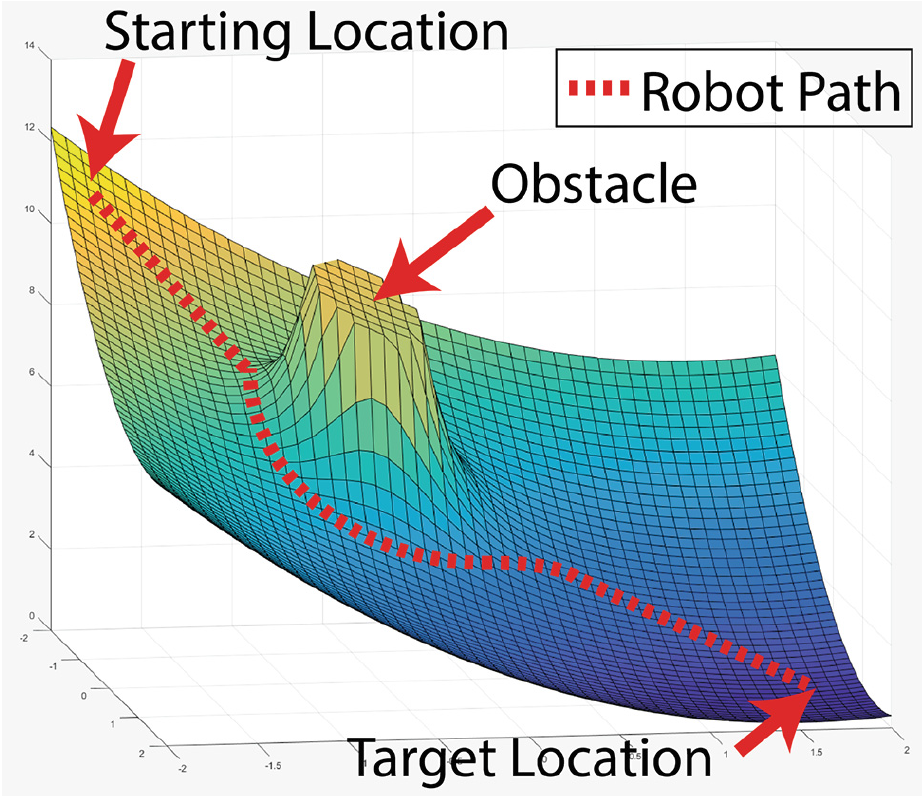
\includegraphics[scale=0.4]{potential_field}
	\caption{Example of artificial potential field}
\end{figure}
Given a point in the Cartesian space a virtual force is generated by the potential field in the direction of the field gradient. 
\begin{equation}
\begin{split}
F^*_{target}&=-grad\left[\mathcal{U_{target}}\right]=-k\left(x-x_D\right)^2 \\
F^*_{obstacle}&=-grad\left[\mathcal{U_{obstacle}}\right]=\begin{cases}\eta\left(\frac{1}{\rho}-\frac{1}{\rho_0}\right)\frac{1}{\rho^2}\frac{\partial\rho}{\partial x}& \text{if } \rho\leq\rho_0 \\
0 & \text{if } \rho>\rho_0
\end{cases}
\end{split}
\end{equation}
Multiple points can be chosen on the manipulator arm, to avoid collisions with all the links of the robot. The forces generated on all of these points are then projected on joint torques space through the Jacobian matrices. This way the manipulator arm, or the mobile robot, is induced by the joint torques to move away from the obstacles.\\
The system subjected to the artificial potential field is stable, but with approach it is very easy to run into local minima where the system is stable, but the robot is not in the target configuration.\\
With systems like Mobile Manipulators the obstacle avoidance problem can also be formulated as an optimization problem. Exploiting its increased number of joints a Mobile Manipulator can follow a primary task, i.e. trajectory traking of the end effector, while simoultaneously optimizing a secondary objective, and/or satisfying certain constraints by utilisation of the system's redundancy. In this sense, obstacle avoidance naturally arises as a secondary objective to be achieved, as explained in \cite{yamamoto2},\cite{tanner2000} or in \cite{perdereau2002}, where an obstacle avoidance term is added in the objective function of the optimization problem for the control of Mobile Manipulators
\begin{equation}
	\varphi_{OA}(q)=\sum_{i=1}^{l}\alpha_ip(\rho_i(q))
\end{equation}
Where $l$ is the number of points where the obstacle avoidance is considered, $\alpha$ is a weighting factor and $p$ is a penalty function depending on the distance of the point from the obstacle.\\
Another approach on Mobile Manipualators obstacle avoidance that deserves to be mentioned is the Elastic Strips method proposed in \cite{brockKhatib} where the motion of the robot is chosen between a set of homotopic collision-free paths through a potential field-based control algorithm. \\
A general issue that each approach has to deal with is the calculation of the minimum distance $\rho$ to an obstacle, and consequently the geometric modelling of the obstacles. More recent obstacle avoidance strategies (\cite{falconatale}) have overcome the complex 3D modelisation of the environment or of the robot. The approach is based on the exploitation of perception data available only from simple proximity sensors distributed on the robot, in order to deviate pre-planned motions exploiting the robot redundancy while executing the primary task. However, this strategy does not guarantee to complete the primary task in any environment.
\subsection{Grasping}
................


%!TEX root = Thesis_main.tex

\chapter{Controller}
\label{chapter5}

\section{Introduction and Aim of the controller}

In this chapter the core of the developed controller will be presented. The goal of our research is to solve the mobile manipulation problem of trajectory tracking for handling and grasping tasks. The tasks we wish to perform are in general solved decoupling the controller in order to move the mobile robot in a defined position in order to have a fixed position of the base during grasping and to reduce uncertainties in end-effector position, and only then perform the grasping task with the manipulator. This approach is generally reliable since controlling independently the base of the robot and the arm with well-known techniques allows precision and robustness. Anyway, if we want to perform the tasks in a time-optimal way this approach is not suitable. The possibility to move within an environment during grasping operation to allow faster performance time is a goal desired not only in manipulation tasks but for many applications. Furthermore, the usage of a unique controller could allow exploiting the many degrees of redundancy to optimize other process variables such as manipulability or obstacle avoidance capability. What we have developed, is a unique controller able to deal with the whole mobile manipulator system. The controller we developed aim is to solve some of the issues presented in Chapter \ref{chapter4} by means of a Nonlinear Model Predictive Control with a novel approach to solve the online optimization problem reducing the overall computational time. The choice of MPC controller has been made for many reasons: 

\begin{itemize}
\item By means of the Receding Horizon Principle (explained in Section \ref{section_MPC}) it is possible to forecast the behaviour of the system. This approach becomes useful for obstacle avoidance and in manipulability maximization tasks.
\item It is an open framework that allows customized problems.
\item Introducing constraints allows taking into account the feasibility set of the joint variable as well as control input limits.
\item Being an Optimal controller allows the minimization of customized parameters such as manipulability, control input effort etc...
\item It is generally used as a high-level controller, the low-level loops are in charge to track given high-level command and deal with system dynamic.
\end{itemize}

In the next section the general NMPC structure for the mobile manipulation problem will be explained referring to a Nonholonomic vehicle and a 6 DOFs manipulator. Our novel approach to reduce computational time and the related stability proof will be discussed later on.

\section{Problem Definition}

In this section the variables of the system and the model used for the MPC problem definition will be defined. The choice of the kinematic model instead of the dynamic one has been made for different reasons:

\begin{itemize}
\item Even if our approach allows to reduce computational time, the usage of the Dynamic model introduce further complexity in system propagation that slow down significantly the solving time.
\item Because the control action of the kinematic model has been defined as velocities, it is easy to implement velocity constraints.
\item Low-level motor controllers are usually in charge to track velocities with higher frequency loops. This hierarchical approach is widely diffuse in controlling complex robotic systems.
\item From a user point of view, kinematic variables allows a better understanding of what is happening on the real system
\end{itemize}

\subsection{Model}

Consider the kinematic relation in \ref{dirkinMM} and the new state variables defined as:
\begin{equation}
{x}(t) \in \mathbb{R}^n\ \  \textnormal{s.t.}\ \  {x}  = \left[ \begin{matrix} x_b \\ y_b \\ \theta_b \\ \Theta_1 \\ \Theta_2 \\ \Theta_3 \\ \Theta_4 \\ \Theta_5 \\ \Theta_6 \end{matrix} \right]\ \   \textnormal{and}\ \  {u}(t) \in \mathbb{R}^m\ \ \textnormal{s.t.}\ \ {u}=\left[ \begin{matrix} v \\ \omega \\ \dot{\Theta}_1 \\ \dot{\Theta}_2 \\ \dot{\Theta}_3 \\ \dot{\Theta}_4 \\ \dot{\Theta}_5 \\ \dot{\Theta}_6 \end{matrix} \right]
\end{equation}
where $\Theta_1, \cdots,\Theta_6$ are the joint values of the manipulator arm.
By means of these variables the nonlinear kinematic model of the Nonholonomic Mobile Manipulator can be defined as:
\begin{equation} \label{system_base}
	\dot{{x}}=f({x},{u})
\end{equation} 
where:
\begin{equation} \label{NLsystem}
	f({x},{u}) = \left[ \begin{matrix}
	G({x}) & \textbf{0} \\ \textbf{0} & I \end{matrix} \right]
\end{equation}
and $G(x)$ is defined as in \ref{Gmatrix_def}:
\begin{equation*}
G({x}) =  \left[
\begin{matrix}
\cos\theta_b & 0 \\
\sin\theta_b & 0 \\
0 & 1 
\end{matrix}
\right] 
\end{equation*}

The continuous time model in \ref{system_base} has been discretized by means of Runge Kutta 4 method. that results in: 

\begin{equation*}
	{x}_{k+1}=f(x_k,u_k)
\end{equation*}
Note that $f$ is now a discretized state equation approximating the \ref{system_base}. Runge Kutta method will be discussed more in details later on.

\subsubsection*{Notation:}
We will use the same notation as in Chapter \ref{chapter3}. Briefly recalling: ${x}_{k|i}$ is the state vector at time instant $i$ propagated starting from time instant $k$, and ${u}_{k|i}$ is defined in the same way.

\subsection{NLP definition}

As done in Chapter \ref{chapter3} we will set up a minimization problem considering a quadratic cost function in the form:
\begin{equation}
J_{k}({x}_{k|i},{u}_{k|i})=\sum_{i=1}^{N}l({x}_{k|i},{u}_{k|i})
\end{equation} 
where $l({x}_{k|i},{u}_{k|i})$ is a positive definite function dependent on the state and the control action. By including Equation \ref{NLsystem} and state and control feasibility boundaries the problem becomes: 
\begin{equation} \label{ourproblem_basic}
\begin{split}
		& min_{\textbf{u}}\ J({x}_{k|i},{u}_{k|i}) \\
		\textnormal{s.t.}\qquad
		&\ \ \ \ x_{k|i+1}=f(x_{k|i},u_{k|i}) \\
		&\ \ \ \ {x}_{k|i} \in \mathbb{X}\ \forall\ i=1,\dots,\ N  \\
		&\ \ \ \ {u}_{k|i} \in \mathbb{U}\ \forall\ i=0,\dots,\ N-1 \\
	\end{split}	
\end{equation}
where $\mathbb{X} = \lbrace {x}\in \mathbb{R}^n\ \textnormal{s.t.}\ {x}_{min}\leq x\leq x_{max} \rbrace$ is the feasible region of the state, $\mathbb{U} = \lbrace {u}\in \mathbb{R}^m\ \textnormal{s.t.}\ {u}_{min}\leq{u}\leq{u}_{max} \rbrace $ and $\textbf{u}=[\ u_{k|0},\ u_{k|1},\ \dots,\ u_{k|N-1}\ ]$.
Note that the problem has to be discretized; we will refer at $T_k$ as the discretization time, so the time between $k$ and $k+1$ as well as the time between $i$ and $i+1$.
The problem defined in \ref{ourproblem_basic} is a standard NMPC problem that can be solved using well-known numerical optimization methods, where Equation \ref{NLsystem} is numerically integrated to propagate the state ${x}_{k|i+1}$. Anyway, the problem so defined is to find a solution $\textbf{u}^* \in \mathbb{R}^{m\times(N-1)}\ \textnormal{s.t.}\ \textbf{u}^* =[{u}^*_{k|0},\ {u}^*_{k|1},\ \dots,\ {u}^*_{k|N-1}]$. Even if, according to MPC logic, only the first computed control action ${u}^*_{k|0}$ will be applied, the problem needs to be solved for all the prediction horizon. Because of that, the dimension of the problem is highly dependent on N. Considering our case, for example, we have $m=8$, so if we set $N=20$ the dimension of $\textbf{u}^*$ that has to be found is $8\times20=160$. The dependence of the problem dimension on the optimization horizon length generate restrictions on the choice of $N$. This is due to the increase in computational effort that may become too high to solve fast online applications like handling and grasping for mobile manipulators. A solution could be to bound the value of $N$ in order to keep the problem within a solvable dimension. However, the performance clearly increases as $N$ increase, allowing compliance with some constraints, like obstacle avoidance, over a longer period. For this reason, we introduced a parameterized control input approach to reduce the dependence of $N$ on the solving time without losing the advantages of a longer prediction horizon.

\subsection{Parameterization}

The problem in \ref{ourproblem_basic} uses a control action defined as piece-wise constant that, as explained before, brings high computational cost dependence on $N$. To solve this issue we propose to express the control vector ${u}_{k|i}$ as a function of some parameters:
\begin{equation}\label{param_eq}
{u}_{k|i}=F(t_i)\textbf{p}_k
\end{equation}
where $\textbf{p} \in \mathbb{R}^{N_p}$ s.t. $\textbf{p}=[\ p_1,\ p_2,\ \dots,\ p_{N_p}\ ]^T$ and the matrix $F(t_i)$ is the base of the new space $\mathbb{R}^{N_p}$. A good choice of the parameterization is made according to the physics of the variables to be parameterized. In \cite{kelly2013mobile} a parametric optimal approach is proposed, anyway, given that the variables to be controlled are longitudinal and angular velocities, a polynomial parameterization can fit the phisical meaning requirement. A better explanation of how to choose the parameterization will be given in Section \ref{stabproof}.
\begin{figure}[h!]
	\centering
	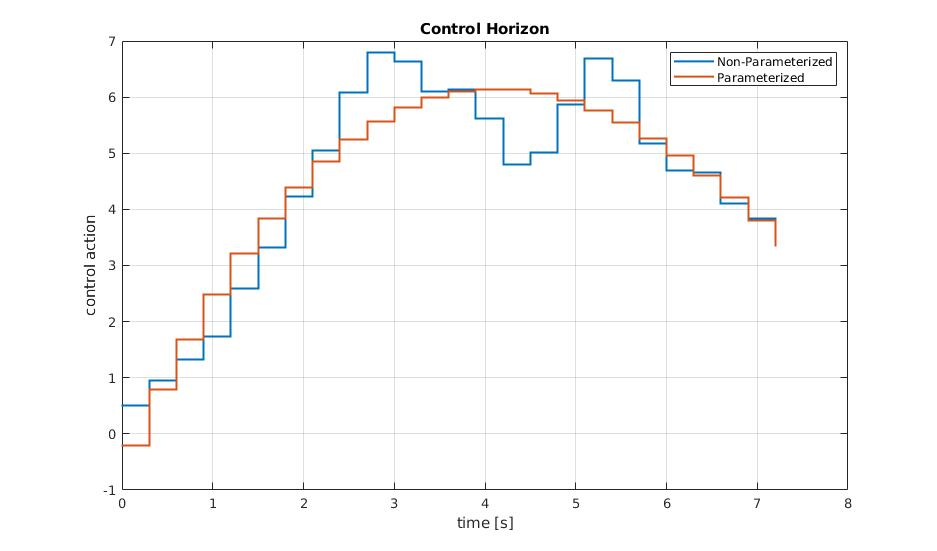
\includegraphics[scale=0.4]{param_horizon}
	\caption{Control input parameterization}
	\label{param_horizon}
\end{figure}
Considering a 3rd order Polynomial parameterization as in Figure \ref{param_horizon} for control input, each row of the ${u}$ vector can be expressed as a function of four parameters, for example $v=p_1t_i^3+p_2t_i^2+p_3t_i+p_4$. More in general ${u}_{k|i}$ is
\begin{equation}
{u}_{k|i}=\left[ \begin{matrix}
H_v(t_i)          & \textbf{0} & \dots      & \textbf{0}  \\
\textbf{0} &     H_\omega(t_i)      & \dots      & \textbf{0}  \\
\vdots     & \vdots     & \ddots     & \vdots      \\
\textbf{0} & \dots      & \textbf{0} &   H_{\Theta_6}(t_i)         \\
\end{matrix} \right] \left[ \begin{matrix} \textbf{p}_v \\ \textbf{p}_{\omega} \\ \textbf{p}_{\Theta_1} \\ \textbf{p}_{\Theta_2} \\ \vdots \\ \textbf{p}_{\Theta_6} \end{matrix} \right]
\end{equation}
where: 
\begin{equation}
\left[ \begin{matrix} \textbf{p}_v \\ \textbf{p}_{\omega} \\ \textbf{p}_{\Theta_1} \\ \textbf{p}_{\Theta_2} \\ \vdots \\ \textbf{p}_{\Theta_6} \end{matrix} \right] = \left[ \begin{matrix} p_1 \\ p_2 \\ p_3 \\ \vdots \\ p_{32} \end{matrix} \right]\ \ \textnormal{and }\ \ H(i)=[\ t_j^3\ \ t_j^2\ \ t_j\ \ 1\ ]
\end{equation}
Note that $t_i$  is defined as:
\begin{equation*}
	t_i=(i-1)T_k\ \ \ \ \forall\ i=1,\dots,N
\end{equation*}
Considering this parameterization, the state equation of the system in \ref{system_base} becomes a LTV system for which the Runge Kutta 4 discretization is done defining: 
\begin{equation*}
\begin{split}
    &k_1 = f(x_{k|i},\textbf{p}_k,t_i) \\
	&k_2 = f(x_{k|i}+k_1\frac{T_k}{2},\textbf{p}_k,t_i+\frac{T_k}{2}) \\
	&k_3 = f(x_{k|i}+k_2\frac{T_k}{2},\textbf{p}_k,t_i+\frac{T_k}{2})\\
	&k_4 = f(x_{k|i}+k_3T_k,\textbf{p}_k,t_i+\frac{T_k}{2})\\
\end{split}	
\end{equation*}
The new state equation becomes:  
\begin{equation}
\begin{split}
	x_{k|i+1}&=x_{k|i}+\frac{T_k}{6}(k_1+2k_2+2k_3+k4) \\
	&=\tilde{f}(x_{k|i},\textbf{p}_k,t_i)
\end{split}
\end{equation}
By applying the change of variables of Equation \ref{param_eq} into the problem formulation in \ref{ourproblem_basic} we obtain:
\begin{equation} \label{ourproblem_param}
\begin{split}
		& min_{\textbf{p}_k}\ J({x}_{k|i},\textbf{p}_k) = \sum_{i=1}^{N}\tilde{l}({x}_{k|i},\textbf{p}_k) \\
		\textnormal{s.t.}\qquad
		&\ \ \ \ x_{k|i+1}=\tilde{f}(x_{k|i},\textbf{p}_k,t_i) \\
		&\ \ \ \ {x}_{k|i} \in \mathbb{X}\quad \forall i=1,\dots, N  \\
		&\ \ \ \ \textbf{p}_k   \in \mathbb{P}\ \\
	\end{split}	
\end{equation}
where $\mathbb{P} = \lbrace \textbf{p}\in \mathbb{R}^{N_p}\ \textnormal{s.t.}\ F(t_j(i))\textbf{p} \in \mathbb{U}\quad \forall i = 1, \dots, N-1 \rbrace $ and $\tilde{l}$ is simply the stage cost defined as a function of $\textbf{p}_k$ instead of ${u}_{k|i}$. By means of this substitution the problem has to be minimized with respect to $N_p$ parameters, whose number do not depend on $N$. As a matter of fact, using 3rd order polynomials as in the previous example, we have to minimize $J$ with respect to $32$ parameters for any length of the prediction horizon. Implementing this approach results in a faster solution of the optimization problem, and the possibility to enlarge significantly the prediction horizon. Anyway $N$ has to be chosen properly: increasing too much the prediction horizon may result in bad performances due to overconstraining of the control action. This effect, as well as a performance comparison with respect to traditional MPC will be discussed later on.


\subsection{Increasing-Weights Cost Function definition}

Once the problem has been defined in its general form we have to properly choose the cost function. In particular, the stage cost $\tilde{l}$ has to be defined. A common choice is to use a quadratic stage cost in order to have a positive definite cost function to help in having a convex problem. Even if it is important to have a quadratic cost function for the stability of the controller, it is still possible to find suboptimal solutions (i.e. local minima) because of the nonlinearities of the system. We will define the stage cost $\tilde{l}$ as a sum of different contributions using increasing weights into the optimization horizon. 
\begin{equation}\label{costfunctionh}
J({x}_{k|i},\textbf{p}_k)=\sum_{i=1}^{N}\left(\frac{i}{N}\right)^m \left[ \sum_{j=1}^{5} h_j({x}_{k|i},\textbf{p}_k) \right]
\end{equation} 
This approach allows, by means of increasing weighted stage costs, to assess the stability of the NMPC without the imposition of terminal constraints, as shown in \cite{alamir2018stability}. This aspect will be reviewed in detail in the following section.
The definition of the functions $h_j$ defines what we want to minimize. Because the aim of the controller is to track the trajectory of the end-effector solving the mobile manipulation problem, the following stage costs are defined.
\begin{itemize}

\item First of all, $h_1$ is the cost related to the end effector pose error defined as: 
\begin{equation}
\begin{split}
h_1 = \left[\begin{matrix} \xi_{k|i}-\xi_{{k|i}_{d}} \\ 1-\Phi_{k|i} \end{matrix}\right]^T W_1\left[\begin{matrix} \xi_{k|i}-\xi_{{k|i}_{d}} \\ 1-\Phi_{k|i}\end{matrix}\right]\textbf{}
\end{split}
\end{equation}
Defining:
\begin{equation} 
\xi_{k|i} = \left[ \begin{matrix} x_{{k|i}_{ee}} \\ y_{{k|i}_{ee}} \\ z_{{k|i}_{ee}} 
\end{matrix} \right] = \left[ \begin{matrix}
1 & 0 & 0 & 0 \\ 0 & 1 & 0 & 0 \\ 0 & 0 & 1 & 0
\end{matrix} \right]A_{{k|i}_{ee}}\left[ \begin{matrix}
0 \\ 0 \\ 0 \\ 1
\end{matrix} \right]
\end{equation} 
and
\begin{equation}
\Phi_{k|i}=\left[\begin{matrix}\vec{\vartheta}_{k|i}\cdot\vec{\vartheta}_{{k|i}_d}\\ \vec{\psi}_{k|i}\cdot\vec{\psi}_{{k|i}_d}
\end{matrix}\right] 
\end{equation}

Where $A_{{k|i}_{ee}}$ is the rototraslation matrix of the end effector with respect to the global reference frame, which is a function of the state $x$;  $\vec{\vartheta}_{k|i}$ and $\vec{\psi}_{k|i}$ are the orientation vectors of the end effector position (i.e. the first and the third columns of $A_{{k|i}_{ee}}$) and $W_1$ is the diagonal weighting matrix for cost $h_1$.

\item In order to maximize the manipulability a cost related to the manipulability of the system is defined as:
\begin{equation}
h_2 = W_2 \left( \frac{1}{m_{k|i}} \right)^2
\end{equation}
with:
\begin{equation}
m_{k|i} =  \det(\mathcal{J}_{ee}^T\mathcal{J}_{ee})
\end{equation}
Where $\mathcal{J}=[\ \mathcal{J}_b(q)\ \mathcal{J}_a(q)\ ]$ i.e. the Jacobians which relates the end effector pose to the joints of the base and of the arm respectively. Like before $W_2$ is a weighting term. As briefly mentioned in Chapter \ref{chapter4}, there are many other ways to express an index for the manipulability of the system. For example, another way this index can be described is with the sine of the elbow joint angle of the manipulator, since the manipulability depends mostly on that angle.
    
\item $h_3$ is the cost related to the control effort defined as: 
	\begin{equation}
	        h_3=\left[ \begin{matrix} v_{k|i-1} \\ \omega_{k|i-1} \end{matrix}\right]^T W_3 \left[ \begin{matrix} v_{k|i-1} \\ \omega_{k|i-1} \end{matrix}\right]
	 \end{equation}
This cost is particularly useful since the higher it is, the less the controller will choose to make adjustments on the end effector position through motions of the base, given that its positioning system is less reliable than the manipulator's one.
\end{itemize}
We will introduce now other two terms that will be used according to the application and in moving the system from and towards the grasping area. Decoupling the problem with two different cost functions allows having a faster controller during the motion of the system when it is required to have high speeds, and to increase the complexity of the problem only inside a grasping area, where the system moves slower, to perform grasping. 
\begin{itemize}
    \item $h_4$ will be used to consider the base positioning error with respect to a given planned trajectory ${x_b}_d$ to reach the grasping area:
        \begin{equation}
            h_4=[x_b-{x_b}_d]^T W_4 [x_b-{x_b}_d]
        \end{equation}
     \item $h_5$ will be used to control the arm in joint space, so to track a desired joint position ${x_a}_d$:
    \begin{equation}
       h_5=[x_a-{x_a}_d]^T W_5 [x_a-{x_a}_d]
    \end{equation}
\end{itemize}
This terms allowing to directly compute the error without passing through the forward kinematics, simplify a lot the problem during the motion of the base permitting a faster computation of the control action.\\We have shown only few terms, but others can also be added to make the controller more completely defined or to make it choose a solution for the kinematic redundancy problem in a different way. 

\section{Stability Proof}\label{stabproof}

Once the NMPC problem has been formulated and that the recursive feasibility of the problem has been easily investigated in Chapter \ref{chapter3}, its stability has to be assessed. 
The proof is very similar to what done in \cite{alamir2018stability} with few modifications. We will consider now, for the stability proof, the tracking problem as a zero-reference tracking problem. In order to do that we will consider:
\begin{equation}
    e_k=x_k-{x_k}_d
\end{equation}
and so, considering the state equation \ref{system_base} in a discretized way, we have:
\begin{equation}\label{sys_eq_con_e}
    e_{k|i+1}=\hat{f}(e_{k|i},p_k,{x_{k|i}}_d,{x_{k|i+1}}_d)
\end{equation}
In this way the problem is moved to track a zero error reference and becomes: 
\begin{equation} \label{ourproblem_stab}
\begin{split}
		& min_{{p}_k}\ J({e}_{k|i},{p}_k) =\sum_{i=1}^{N}\hat{l}(e_{k|i},{p}_{k}) \\
		\textnormal{s.t.}\qquad
		&\ \ \ \ e_{k|i+1}=\hat{f}(e_{k|i},p_k) \\
		&\ \ \ \ e_{k|i} \in \mathbb{E}\ \forall\ i=1,\dots,\ N  \\
		&\ \ \ \ {p}_k\   \in \mathbb{P}\ \\
	\end{split}	
\end{equation}
where $\mathbb{E} = \lbrace {e}\in \mathbb{R}^n\ \textnormal{s.t.}\ {e}_{min}\leq e\leq e_{max} \rbrace$ is the feasible region of the state error. Note that, for simplicity of notation, the system equation in \ref{sys_eq_con_e} has been expressed as a function of the previous state ${x_{k|i}}$ and the parameters $p_k$ only, given that the desired states are known.
Now, following the demonstration in \cite{alamir2018stability} we need to introduce some assumptions in order to assess stability of the controller. The proof will consider some modification of what done in \cite{alamir2018stability} to consider the parametrization of the control input. 

\paragraph{Assumption 1} The maps of $\hat{f}$ and $\hat{l}$ are continuous and $\hat{l}$ is a positive definite function. 

\paragraph{Assumption 2} We will introduce also a reachability requirement, so that $\exists \textnormal{ a set } \mathbb{E}_N$ so that $\forall e \in \mathbb{E}_N $ the set:
\begin{equation*}
	\mathbb{P}_{e \to 0}:=\lbrace \ p \in \mathbb{P}\ \text{s.t.}\ e_{N}(e,p)=0\ \rbrace
\end{equation*} exist and is not empty.

\paragraph{Assumption 3} Local control invariance is assumed in the neighborhood of the origin, i.e. there exsist a $\bar{\rho} > 0$ such that:
\begin{equation}
	\begin{split}
		\forall \rho &\leq \bar{\rho},\ \forall e \in B_{\it{l}}(\rho),\ \exists\ p^+\ 	 \textnormal{s.t.} \\
		&\hat{l}\left(\hat{f}\left(e\left(p\right)\right)\right)-\hat{l}\left(e\right) \leq -q(e) 
		\label{ass3}
	\end{split}
\end{equation}
for some positive definite function $q$ that satisfy:
\begin{equation}
	q(e) \ge \gamma l(e)
	\label{ass3_1} 
\end{equation}
for some $\gamma \geq 0$ and $\forall x \in \mathbb{X}$.
Where $B_{\it{l}} \subset \mathbb{R}^n$ is the $\rho-$level set of $l$, defined as $B_{\it{l}} := \lbrace\ e \in \mathbb{R}^n\ |\ l(e) \leq \rho \rbrace$.

\paragraph{Assumption 4} We will require an extended control input parameterization vector $p:=[p_1,\ p_2,\ \dots,\ p_{N_p},\ \kappa]$ such that: 
\begin{equation}
\begin{split}\label{new_parameterization}
    u_{k|j}(p_k)=
        \begin{cases}
            F(j){p_k}\ \ \ \ \   &\textnormal{if } j<\kappa \\
            \bar{u}=argmin_u l(\hat{f}(e_{k|N},u_k))\ \ &\textnormal{if } j\ge \kappa
        \end{cases}
    \end{split}
\end{equation} 
Then given the optimal solution at time instant $k$ defined as $$p_k^*=\left[ p_{k_1}^*,\ p_{k_2}^*,  \dots,\ p_{k_{N_p}}^*,\ \kappa^* \right]^T$$ that corresponds to $  \textbf{u}_k^*=[\ u_{k|0}^*,\ u_{k|1}^*,\  \dots,\  u_{k|{N-1}}^*\ ]$ it is possible to obtain the parameters $\tilde{p}_{k+1}$ such that the correspondent control input is $  \tilde{\textbf{u}}_{k+1}=[\ u_{k|1}^*,\ u_{k|2}^*,\  \dots,\  u_{k|{N-1}}^*,\ \bar{u} \ ]$. This is better understandable looking to Figure \ref{param_translatability}: if at time instant $k$ the computed optimal solution is represented by the blue line, the suboptimal solution $\tilde{p}_{k+1}$ for the optimization problem at time instant $k+1$ is the one described by the same blue line followed by the red one ($\bar{u}$).
That means to require that the parameterization function \ref{new_parameterization} has to be translatable.
\begin{figure}[h!]
	\centering
	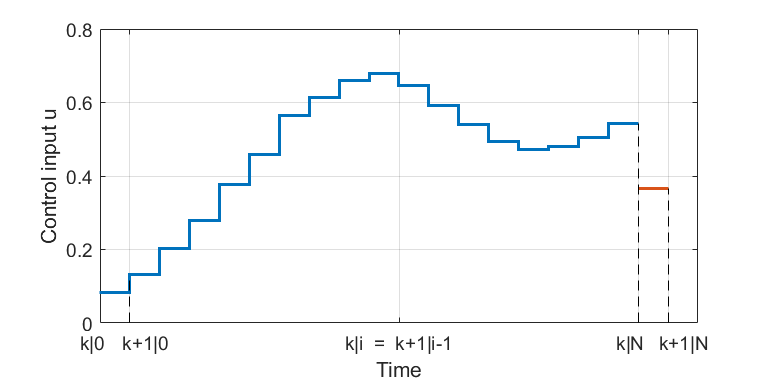
\includegraphics[scale=0.6]{IMMAGINI/trans_u.png}
	\caption{Translatability of the $F$ function}
	\label{param_translatability}
\end{figure}

\paragraph{Lemma 1} Under Assumption 1, $\forall e \in \mathbb{E}^N$, one has:
\begin{equation}
	l(e_N(p^*)) \leq \eta\ c^m\ \ \  \textnormal{where    } c:=\frac{N-1}{N} < 1
 	\label{lemma1}
\end{equation}
for some bounded $\eta < 0$. The proof of Lemma 1 is given in \cite{alamir2018stability}. \\

In order to assess stability is required that the cost function $J({e}_{k|i},{p}_k)$ is proven to be a Lyapunov function as explained in Chapter \ref{chapter3}. So, considering the cost function related to $\tilde{p}_{k+1}$ is:
\begin{equation*}
    J({e}_{k+1|i},\tilde{p}_{k+1})=\sum_{i=1}^{N-1}\left(\frac{i}{N}\right)^m h({e}_{k|i},\tilde{p}_{k+1})+h(\hat{f}(e_{k|N},\bar{u}))
\end{equation*}
Now considering $j=i+1$ and a simplified notation $h({e}_{k|i},p_{k}^*)=h(e_{k|j})^*$, it follows: 
\begin{equation*}
    J({e}_{k+1|i},\tilde{p}_{k+1})=\sum_{j=2}^{N}\left(\frac{j-1}{N}\right)^m h(e_{k|j})^*+h(\tilde{f}(e_{k|N},\bar{u}))
\end{equation*}
Now rearranging the terms: 
\begin{equation*}
    \begin{split}
        J({e}_{k+1|i},\tilde{p}_{k+1})=&\sum_{j=2}^{N}\left[\left(\frac{j-1}{N}\right)^m-1\right]\left(\frac{j}{N}\right)^m h(e_{k|j})^*+ \\
        &+\sum_{j=2}^{N}\left(\frac{j}{N}\right)^m h(e_{k|j})^* + h(\hat{f}(e_{k|N},\bar{u}))
    \end{split}
\end{equation*}
Note that 
\begin{equation*}
	\sum_{j=2}^{N}\left(\frac{j}{N}\right)^m h(e_{k|j})^*=J({e}_{k|i},p_{k}^*)-\frac{1}{N^m}h(e_{k|1})^*
\end{equation*}
So we get:
\begin{equation*}
    \begin{split}
        J({e}_{k+1|i},\tilde{p}_{k+1})=&J({e}_{k|i},p_{k}^*)-\frac{1}{N^m}h(e_{k|1})^*+ \\ 
        &-\sum_{j=2}^{N}\left[1-\left(\frac{j-1}{N}\right)^m\right]\left(\frac{j}{N}\right)^m h(e_{k|j})^*+ h(\hat{f}(e_{k|N},\bar{u}))
    \end{split}
\end{equation*}
And because $\forall j \in \lbrace2,\ \dots,\ N\rbrace$ holds that: 
$\left[ 1-\left(\frac{j-1}{N}\right)^m \right]\ge\left[ 1-\left(\frac{N-1}{N}\right)^m \right]= \phi(m)$. We can then say that: 
\begin{equation}\label{dim1}
    \begin{split}
        J({e}_{k|i},\tilde{p}_{k+1})\le &J({e}_{k|i},p_{k}^*) - \frac{1}{N^m}h(e_{k|1})^*+ \\ 
        &-\phi(m)\sum_{j=2}^{N}\left(\frac{j}{N}\right)^m h(e_{k|j})^*+ h(\hat{f}(e_{k|N},\bar{u}))
    \end{split}
\end{equation}

Now according to Lemma 1, $e_N(p^*) \in B_l(\eta c^m)$ and together with Assumption 2 implies that for $m$ sufficiently high, it is possible to say:
\begin{equation}
\eta c^m \leq \bar{\rho}
\end{equation}

where $\bar{\rho}$ is the positive real called in Assumption 3.
This means that \ref{ass3} holds for $e_N(p^*)$ and we can say that:
\begin{equation*}
    h(\tilde{f}(e_{k|N},\bar{u})) \le h(e_{k|N})^*-q(e_{k|N},p_k^*)
\end{equation*}
By applying this relation on the \ref{dim1} we obtain: 
\begin{equation*}
    \begin{split}
        J({e}_{k|i},\tilde{p}_{k+1})\le &J({e}_{k|i},p_{k}^*) - \frac{1}{N^m}h(e_{k|1})^*+ \\ 
        &-\phi(m)\sum_{j=2}^{N}\left(\frac{j}{N}\right)^m h(e_{k|j})^*+ h(e_{k|N})^*-q(e_{k|N},p_k^*)
    \end{split}
\end{equation*}
Then using Equation \ref{ass3_1}:
\begin{equation*}
    \begin{split}
        J({e}_{k|i},\tilde{p}_{k+1})&\le J({e}_{k|i},p_{k}^*) - \frac{1}{N^m}h(e_{k|1})^*+ \\ 
            &-(\phi(m)-1+\gamma)\ h(e_{k|N})^*
    \end{split}
\end{equation*}
Noting that $\phi(m) \rightarrow 1$ for $m \rightarrow \infty$, for sufficiently high values of $m$, $J$ is a Lyapunov function. It follows that the closed loop system is asymptotically stable in $e=0$.

\section{Constraints}

Constraints will be introduced in order to properly define the problem taking into account feasibility configurations, maximum velocities and accelerations as well as to avoid self-collision of the system. In particular, the constraints definition has been divided into: 

\subsubsection*{Joint position constraints}
	To limit the configurations of the robot into feasible sets and to avoid the arm to self collide there are different approaches. We decided to limit the possible positions of the joints of the arm into feasible ranges. This means to generate a set:
	\begin{equation}
		\mathbb{R}^{x_a}:=x_a \in \mathbb{R}^{x_a}\ \ \text{s.t.}\ \  {x_a}_{min}\ \leq\ x_a\ \leq\ {x_a}_{max} 
	\end{equation}
	Applying this constraint into the MPC problem defined in Equation \ref{ourproblem_param} is straigthforward given that $\mathbb{R}^{x_a}$ is a subset of $\mathbb{X}$.
\subsubsection*{Base position constraints}
	Contrary to the manipulator, self-collision of the base of the system is not possible and the joint $q_b$ could remain unconstrained. Anyway, the $x$ and $y$ coordinates of the base have been limited to define a region of operation for the Mobile Manipulator, see as example figure \ref{xy_limits}. This constraint is particularly useful performing experiments defining a map of the surrounding environment. As before: 
	\begin{equation}
		\mathbb{R}^{x_b}:=x_b \in \mathbb{R}^{x_b}\ \ s.t.\ \  {x_b}_{min}\ \leq\ x_b\ \leq\ {x_b}_{max} 
	\end{equation}

	\begin{figure}[h!]
	\centering
	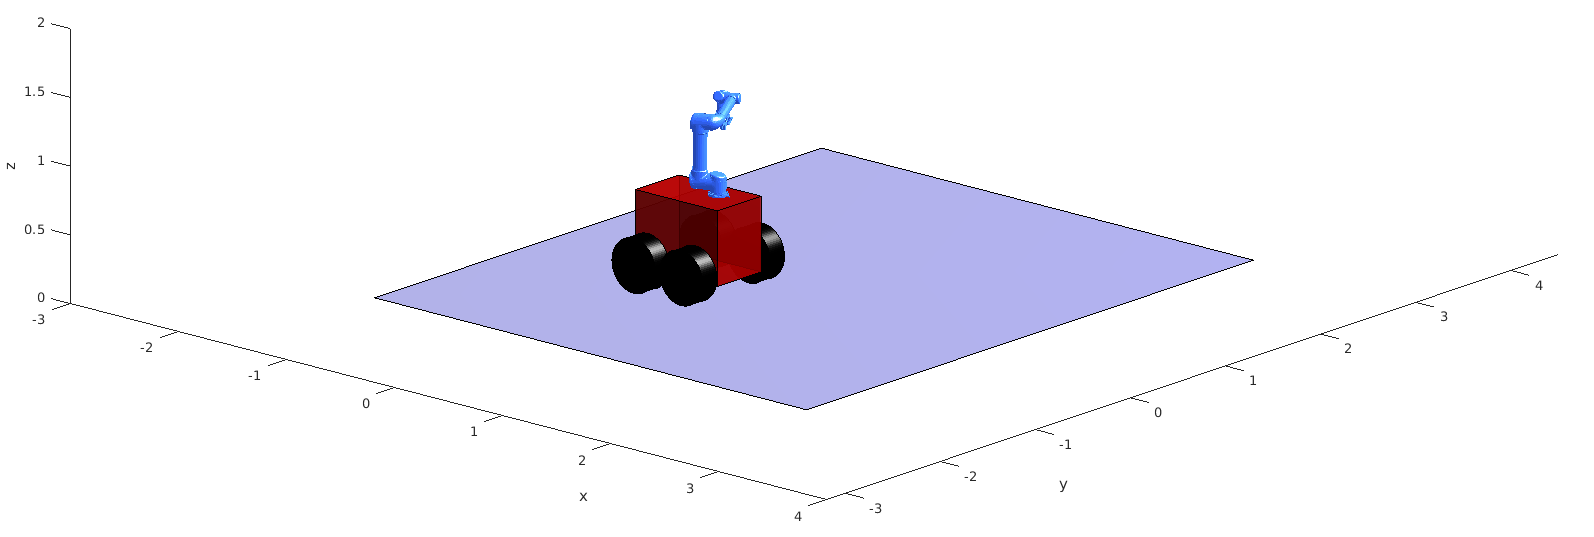
\includegraphics[scale=0.25]{IMMAGINI/xy_limits.png}
	\caption{Base $x-y$ limits}
	\label{xy_limits}
	\end{figure}

	Base and joints position constraints can be written in a compact form and for the entire prediction horizon redefining: 
	\begin{equation}
	\mathbb{X}:= x \in \mathbb{R}^{n}\ \ \text{s.t.}\ \  {x}_{min}\ \leq\ x\ \leq\ {x}_{max}
	\end{equation}

\subsubsection*{Velocity constraints}
	To take into account the maximum velcities allowed by the system, the control actions have been limited into minimum and maximum velocities according to manufacturer data in particular $\mathbb{R}^m$ have been redefined as:
	\begin{equation}
	\mathbb{R}^m:=\ {u}_{k|i} \in \mathbb{R}^m\ \ \textnormal{s.t.}\ \ u_{min}\leq{u_{k|i}}\leq u_{max}\ \ \forall i=0,\dots, N-1
	\label{vel_constr}
	\end{equation}
	According to the parameterization chosen, the constraint has to be defined in parametric form, i.e. we have to map $\mathbb{R}^m$ in $\mathbb{P}$. The constraint to be included in the problem in Equation \ref{ourproblem_param} requires that:
	\begin{equation*}
		\mathbb{P}:=p_k \in \mathbb{P}\ \textnormal{ s.t. Eq.\ref{vel_constr} is satisfied}
	\end{equation*}

	Numerical values will be given in the next section.
\subsubsection*{Acceleration constraints}
	Given that any real system is not capable to perform infinite accelerations, a constraint to limit the computed velocity control input has to be defined. In particular, given that the controller compute control actions with a frequency $f_c=\frac{1}{T_k}$, the acceleration constraint is in the form:
	\begin{equation}
		\begin{split}
			\lvert u_{k|0}\rvert &\leq \lvert u_{k-1|0}\rvert + a_{max} T_k\qquad \textnormal{and}\\
			\lvert u_{k|i+1}\rvert &\leq \lvert u_{k|i}\rvert + a_{max} T_k\quad  \forall i=0,\dots,N-1
		\end{split}	
	\end{equation}  

	where $a_{max}$ is the vector of the maximum allowable acceleration. Numerical values will be given in the next section. 

\subsubsection*{Self collision avoidance}
	To avoid self collosion of the system (i.e. the arm with the base), an approach similar to the one in \cite{sandberg1988collision} has been used. In particular spheres to encompass the base and the last joints have been defined as in Figure \ref{spheres_3d}.
	\begin{figure}[h!]
	\centering
	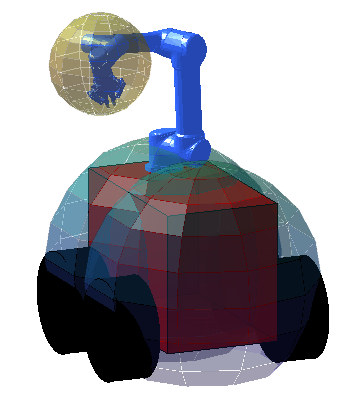
\includegraphics[scale=0.4]{IMMAGINI/spheres_3d.png}
	\caption{Spheres for self collision avoidance}
	\label{spheres_3d}	
	\end{figure}
	Formally the self collision avoidance constraint has been defined requiring that: 
	\begin{equation}
	\begin{split} 
		&\sqrt{({C_0}_x-{C_1}_x)^2+({C_0}_y-{C_1}_y)^2+({C_0}_z-{C_1}_z)^2} + r_1 +r_0 \geq 0 \\
		&\ \ \ \ \textnormal{and} \\
		&\sqrt{({C_0}_x-{C_2}_x)^2+({C_0}_y-{C_2}_y)^2+({C_0}_z-{C_2}_z)^2} + r_2 +r_0 \geq 0 \\
	\end{split}
	\label{spheres_const}
	\end{equation}
	where ${C_0}_{x,y,z},{C_1}_{x,y,z} \text{and }{C_2}_{x,y,z}$ are the coordinates of the centres of the end effector and base spheres respectively defined in the reference frame of the base and $r_1$ and $r_2$ are their radii. This constraints definition introduces a nonlinear equation that has to be satiflied in the solution of the \ref{ourproblem_param}. \\

Summarizing, the presented constraints redefines the problem as:
\begin{equation} 
	\begin{split}
			& min_{\textbf{p}_k}\ J({x}_{k|i},\textbf{p}_k) = \sum_{i=1}^{N}\tilde{l}({x}_{k|i},\textbf{p}_k) \\
			\textnormal{s.t.}\qquad
			&\ \ \ \ x_{k|i+1}=\tilde{f}(x_{k|i},\textbf{p}_k,t_i) \\
			&\ \ \ \ {x}_{min}\ \leq\ x_{k|i}\ \leq\ {x}_{max}\  \forall\ i=1,\dots,\ N  \\
			&\ \ \ \ 0 \leq g^{sc}_{k|i}(x)\ \ \forall\ i=1,\dots,\ N \\
			&\ \ \ \ \textbf{p}_k\   \in \mathbb{P}\ \\
	\end{split}	
	\label{ourproblem_param_vinc}
\end{equation}
where $g^{sc}_{k|i}(x)$ is the function that defines the spheres constraints as in \ref{spheres_const}


%!TEX root = Thesis_main.tex

\chapter{Experimental Setup}
\label{chapter6}

The Mobile Manipulator under analysis in this thesis is a prototype assembled at the University of Southern California in the Center of Advanced Manufacturing (CAM) Laboratory. The system has been called ADAMMS (Agile  Dexterous  Autonomous  Mobile Manipulation System) and it is shown in Figure \ref{imgADDAMS1}.

\begin{figure}[h!] 
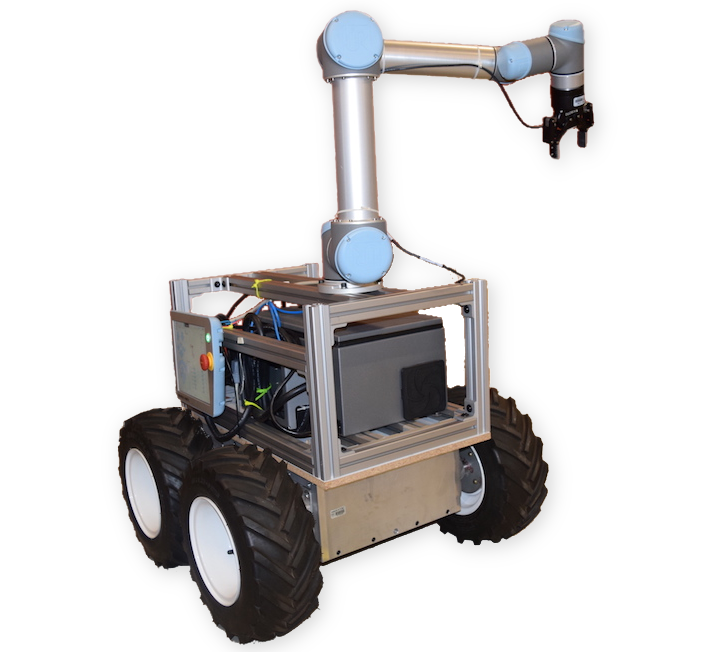
\includegraphics[scale=0.25]{ADDAMS1}
\centering
\caption{ADAMMS}
\label{imgADDAMS1}
\end{figure}

The goal of this prototype is to study a system able to handle parts as well as to perform operations in unstructured industrial environments to fill the gap between small and large production systems. Indeed, companies with small production volumes are nowadays required to innovate production systems towards the generation of smart factories. Given that those companies are generally not economically able to manage automated production lines and that the production mix is generally changed frequently, flexible systems to support production are required. For those reasons ADAMMS wants to be a low-cost solution, using low-cost sensors and to be capable, once its operation has been planned, to perform tasks in any environment. \\


The controller presented in this thesis wants to be the first step towards the design of an online software that makes the system able to operate autonomously once the task has been given. In the next sections the main components of ADAMMS will be shown in its Hardware and Software parts; then setups used for simulations and physical tests will be presented. 
\section{Hardware}

\subsection{Mobile Base}

\begin{figure}[h]
\begin{center} 
	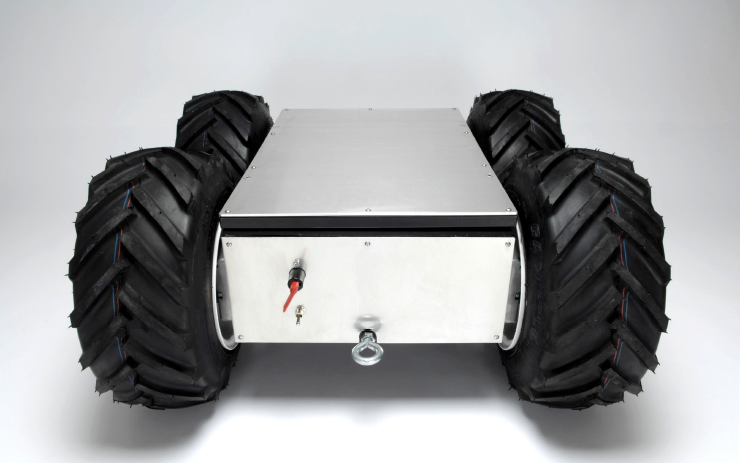
\includegraphics[scale=0.6]{SuperMegaBot1}
	\centering
	\caption{Nonholomic Mobile base}
	\label{fig:SuperMegaBot1}
\end{center}
\end{figure}
The mobile base shown in Figure \ref{fig:SuperMegaBot1}, provided by InspectorBots and named Super Mega Bot (SMB), is a Heavy-Duty, All-Terrain, 4WD robotic platform. It is a rugged, indoor/outdoor platform and can be fitted with a variety of sensors, cameras and equipment. The base has been designed to be modular and reconfigurable, so an end user can swap out various modules. There are several methods available provided by the manufacturer to control the SMB including RC radio, Analog Joystick, Wireless Modem, or Microcomputer.\\
The SMB is designed with non-steering coupled wheels and because of that the rotation of the base is obtained giving different velocities to the right and left wheels. For this reason, the SMB is configured as a differential-drive mobile robot for which the kinematic relationships explained in Chapter \ref{chapter2} hold. This particular mobile platform has been chosen for its high payload and because it is large enough to keep on its upper surface the UR5 control unit. In Appendix \ref{AppA} technical data of the SMB and information about the motors used can be found.

\subsection{UR5 Manipulator}
The UR5 is a collaborative robotic arm developed by Universal Robots. According to the company, the key benefits of their robots are lightweight, safety and easiness to use. The robotic arm is regarded as safe because it will stop acting as soon as the robot hits an object sensed by a force sensor in one of the joints. UR5 is ideal for automating low-weight processing tasks like picking, placing and testing. The medium-sized robot arm is easy to program, fast to set up and, always according to UR, offers one of the fastest payback times in the industry. Because it is designed as a collaborative robot, the UR5 is generally suitable for tasks in which the operative space of the robot is shared with humans and that fits also ADAMMS objectives. The UR5 comes from the manufacturer with its control unit that can be easily accessed and provides low-level controllers for tracking velocities of the joints. More technical details on UR5 can be found in Appendix \ref{AppB}.
\begin{figure}[htbp]
\begin{center} 
	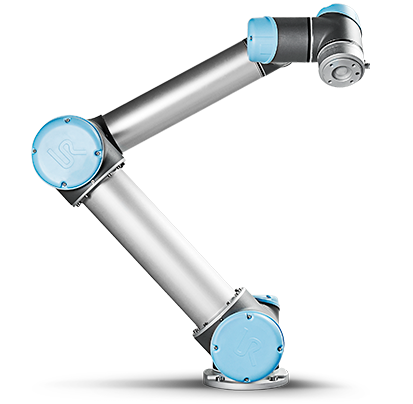
\includegraphics[scale=0.4]{UR5}
	\centering
	\label{fig:UR5}
	\caption{UR5 robot arm} 
\end{center}
\end{figure}
\subsection{Sensors}
The sensors of the ADAMMS prototype are used to measure the positions of the joints, in order to perform the desired task. Briefly, the sensor system is composed of:
\begin{itemize}
\item angular encoders for the UR5 joints, which provide an accuracy of $0.1$ mm at the end effector position;
\item encoders on the wheels of the base, that will be used to derive the position and orientation of the mobile base through a simple transformation.
\begin{equation*}
\begin{split}
\dot{\theta}_b=&\frac{r(\omega_R-\omega_L)}{d} \\\\ \dot{x}_b=\frac{r(\omega_R+\omega_L)}{2}\cos\theta_b &\qquad \dot{y}_b=\frac{r(\omega_R+\omega_L)}{2}\sin\theta_b
\end{split}
\end{equation*}
This measuring system is reliable only at slow speed and provides an accuracy of $\pm 2$ cm. Since the position of the end effector is computed knowing the position of the base, the accuracy of these measures is not sufficient to perform precise operations. Considerations on this aspect will be done later on.
\item a lidar that can be used to measure unknown obstacles position in the operative area of the robot.
\item a Kinect sensor for Simultanous Localization And Mapping (SLAM)
\end{itemize}

\section{Software}

To easily interface with all the components of ADAMMS we used ROS, an open-source, meta-operating system for robotic systems. ROS provides the services that allow communication between all the components, message-passing between processes, hardware abstraction, low-level device control. It also provides tools and libraries for obtaining, building, writing, and running code across multiple computers. The ROS network used to run the physical system is shown in the graph of Figure \ref{ROSnodes}
\begin{figure}[h!]

\makebox[\textwidth][c]{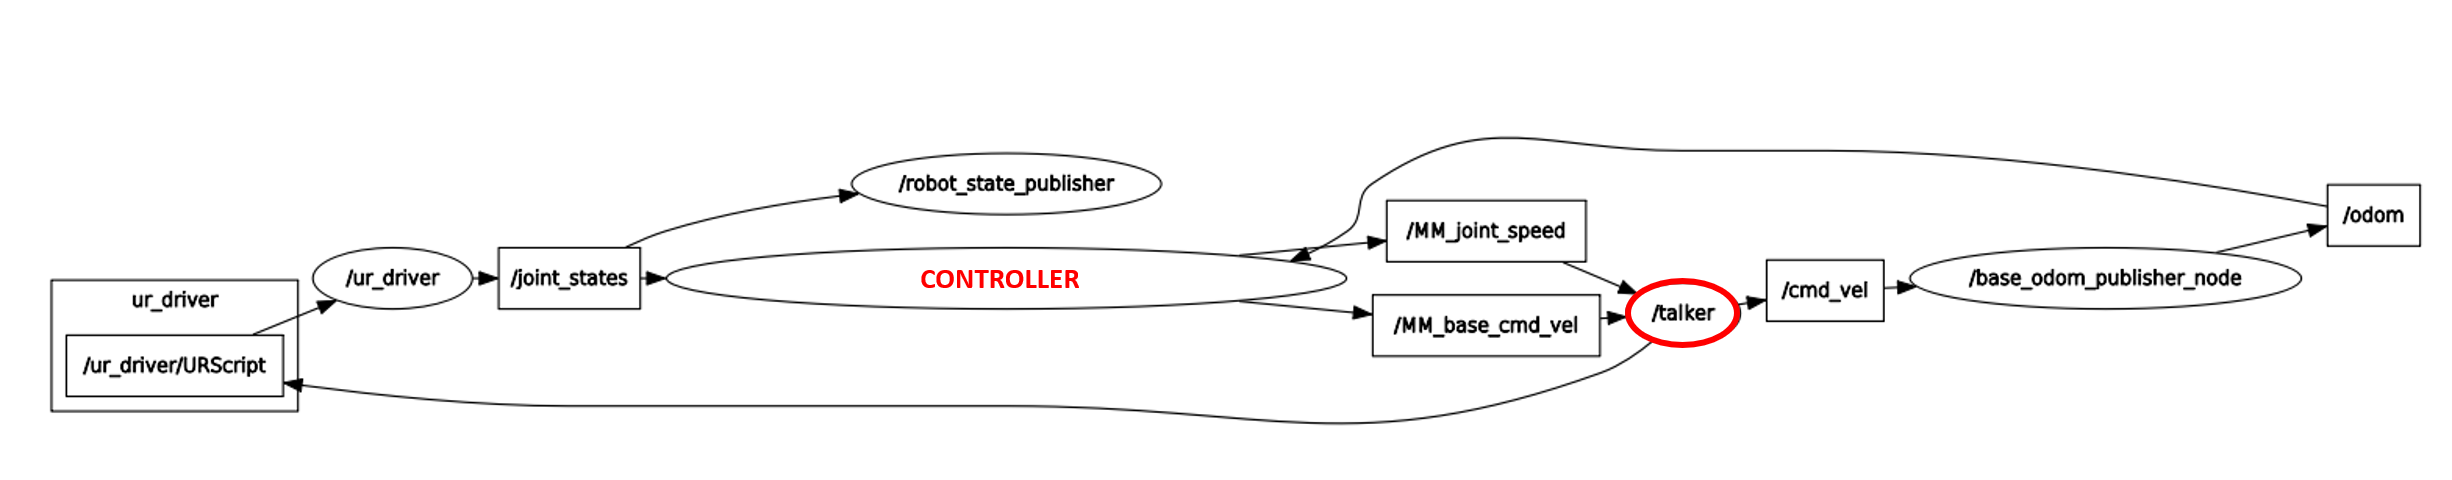
\includegraphics[scale=0.4]{nodegraph1}}
\centering

\caption{ROS nodes and messages for ADAMMS}
\label{ROSnodes} 
\end{figure}

The controller we designed has been developed using Matlab/Simulink environment through CasADi, an open-source tool for nonlinear optimization and algorithmic differentiation that allows using Matlab/Simulink to define optimization problems and different commercial solvers. More information about CasADi can be found in \cite{Andersson2018}. The solver used to solve the Nonlinear Problem described in Chapter \ref{chapter5} is IPOPT; a brief introduction to IPOPT can be found in Appendix \ref{AppC}. As shown in the graph of Figure \ref{ROSnodes}, the Simulink node where the controller is running, reads position of the base and joint angles from the corresponding node, and give velocity commands to the system through a "talker" node that we defined to communicate with the robot. As already mentioned, the commands given to the system are velocity commands, i.e. high-level commands that the system is required to track. Anyway, given that the manufacturers already provides reliable low-level controllers able to track those desired velocities, we decided to use, as mentioned in Chapter \ref{chapter5}, a hierarchical approach that is briefly explained in Figure \ref{Hdiagram}.  
\begin{figure}[h!]

	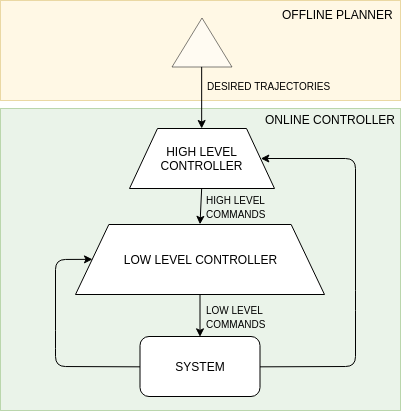
\includegraphics[scale=0.5]{Hdiagram}
	\centering
	
	\caption{Control hierarchy} 

\label{Hdiagram}
\end{figure}
\\
Simulations and physical experiments have been carried out to test the developed controller and to analyze performances and influences of parameters. In particular two tasks have been tested: 

\begin{itemize}
\item \textbf{Movement of the system toward/from the grasping area}. Referring to the controller as presented in Chapter \ref{chapter5} we will consider the cost function expressed in Equation \eqref{costfunctionh} as a composition of $h_4$ and $h_5$. Indeed, the task of moving the system towards the grasping area is performed controlling the base and joint angles positions without requiring to track the end effector position. The choice of this formulation for the cost function allows the problem to be easier to solve given that we are tracking joint angles rather than compute through forward kinematics the end effector position. Furthermore, the arm is generally not required to move during the motion of the system.

\item \textbf{Trajectory tracking inside grasping area}. In this case we will consider the problem of tracking the end effector position considering the cost function \eqref{costfunctionh} as a composition of $h_1$, $h_2$ and $h_3$, and eventually $h_4$ in the cases when the base is required to not stop. This task is more of interest for this thesis and then will be discussed more in detail. Considerations about online changing the cost function will be given in the next chapter. 
\end{itemize}
\section{Simulations setup}

Simulations for both the tasks object of study have been performed using Simulink to test stability, robustness, performance and effects of the parameters on the controller. The model used to simulate the system is basically the same presented in Chapter \ref{chapter2}, computing the state of the system through numerical integration. The block diagram in Figure \ref{simdiagram1} shows the simple architecture of the controller used in simulations.

\begin{figure}[h!]
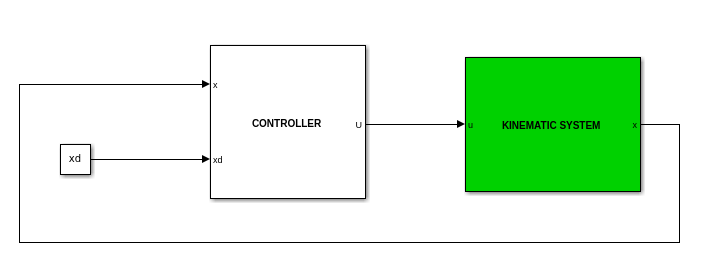
\includegraphics[scale=0.45]{simdiagram1}
\centering
\caption{Simulations block diagram} 
\label{simdiagram1}
\end{figure}

The results of the simulations have been saved and processed in MATLAB R2018b. The solver for the optimization problem (IPOPT) works at a given frequency $f_c=\frac{1}{T}$. Each time the solver is called, as we see in Equation \eqref{ourproblem_param_vinc}, four terms are needed to compute a new control action: 
\begin{itemize}
\item $x_{k|0}$: the state measured at time instant $k$, used as a starting point to propagate the future states;
\item ${x_{k|i}}_d \ \ \forall i=1,\dots,N$: the desired states for the control horizon;
\item $u_{k-1|0}$: needed to compute the velocity constraint at time step $i=0$;
\item $p_0$: the initial guess of the parameters to be estimated solving the problem.
\end{itemize}
Referring to this last term $p_0$, the value has been chosen, both for simulations and physical experiments, equal to zero at the initial time (i.e. a vector of zeros). For all the other calls of the solver $k\neq0$, the previous optimal solution $p_{k-1}^*$ has been given. This choice generally helps to find the solution faster, given that the previous solution is usually not so far from the new one.
\begin{figure}[h!]
	
	\makebox[\textwidth][c]{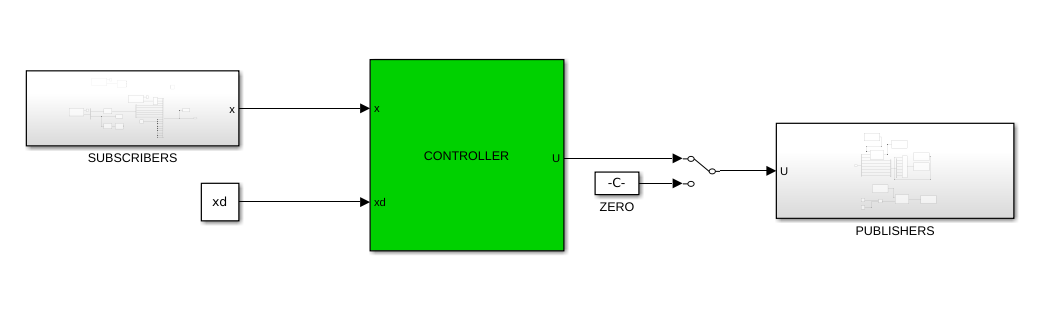
\includegraphics[scale=0.4]{diagramreal}}
	\centering
	
	\caption{Physical experiments block diagram} 
	
	\label{diagramreal}
\end{figure}
\section{Physical Experiments Setup}
The software setup for the physical experiments, as anticipated, makes use of ROS to interface with the real system. In particular, the controller node has been created in Simulink by means of the Robotic System Toolbox provided by Mathworks. The control input velocities have been given to the system by means of a communication node to interface with the low-level controllers. Figure \ref{diagramreal} shows the architecture of the controller used for physical experiments.



%Performances of the low-level controller have been tested primarily giving step input velocities commands to test the response of the base and the arm joints. In Figure \ref{testllbase} and \ref{testllarm} are reported the step responses of the base linear velocity $v$ and the joint angle velocity $\dot{\Theta}_3$ respectively.
%\begin{figure}[ht]
%\centering
%\subfigure[Base step response]{%
%\label{testllbase}%
%
\includegraphics[scale=0.15]{empty}}%
%\qquad
%\subfigure[Arm joints step response]{%
%\label{testllarm}%
%
\includegraphics[scale=0.15]{empty}}%
%\caption{Low level controllers step response}
%\end{figure}
%The measurements of the performed velocity for these tests have been derived from joints encoders for the arm and encoders on the wheels for the base. Since the main aim of the low-level robot controllers is to track some velocity profile, after testing the step response, the tracking of a simple sine trajectory has been analyzed. In Figures \ref{testllbase2} and \ref{testllarm2} are reported the results.
%\begin{figure}[ht]
%\centering
%\subfigure[Base sine response]{%
%\label{testllbase2}%
%
\includegraphics[scale=0.15]{empty}}%
%\qquad
%\subfigure[Arm joints sine response]{%
%\label{testllarm2}%
%
\includegraphics[scale=0.15]{empty}}%
%\qquad
%\subfigure[Base tracking error]{%
%\label{testllbase3}%
%
\includegraphics[scale=0.15]{empty}}%
%\qquad
%\subfigure[Arm joints tracking error]{%
%\label{testllarm3}%
%
\includegraphics[scale=0.15]{empty}}%
%\caption{Low level controllers trajectory tracking}
%\end{figure} \\
%The errors with respect to those trajectories are shown in \ref{testllbase3} and \ref{testllarm3}. We can see that the responses show an overdamped behaviour. Indeed, robot low-level controllers are always overdamped, although the ideal case will be a critically-damped system.  If the system would be underdamped the behaviour of the system can lead to overshoots that are generally not desired in robotic applications. At the same time if the system is too much overdamped the robot movement becomes very sluggish. Hence most controllers are designed to give a near critically-damped response.
%!TEX root = Thesis_main.tex

\chapter{Results}
\label{chapter7}
\section{Simulations results}
\begin{floatingfigure}[r]{.33\textwidth}
	\centering
	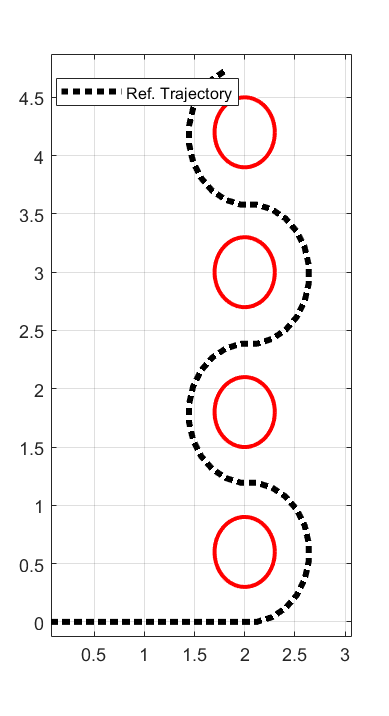
\includegraphics[scale=0.4]{traj_base_curves}
	\caption{Base trajectory for simulations: radius of the curve = 0.6m\label{traj_base_curves}}
\end{floatingfigure}
The goal of the initial simulations is to assess the actual convenience of our approach and to tune the MPC parameters and weights. Once achieved good performances with a proper set of parameters, the controller can be tested with the physical system.\\
Initially some simulations with only the mobile base have been run on a trajectory with low-radius curves (in Figure \ref{traj_base_curves}), seeing the effect of different control horizon lengths and of input disturbances. This trajectory has been chosen to simulate how our controller tracks a trajectory which goes around some obstacles. No obstacle avoidance is considered in this simulation.
\begin{figure}[!h]
	\centering
	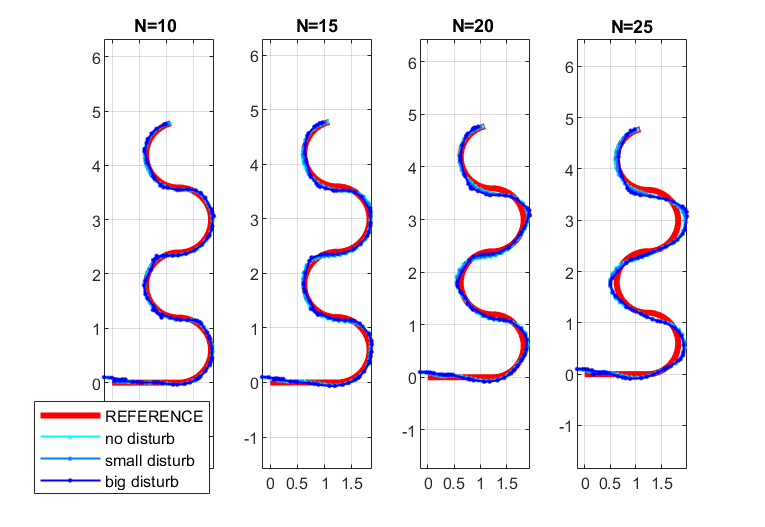
\includegraphics[scale=0.5]{base_curves}
	\caption{Mobile platform trajectories with different N}
	\label{base_curves}
\end{figure}
\begin{figure}[!h]
	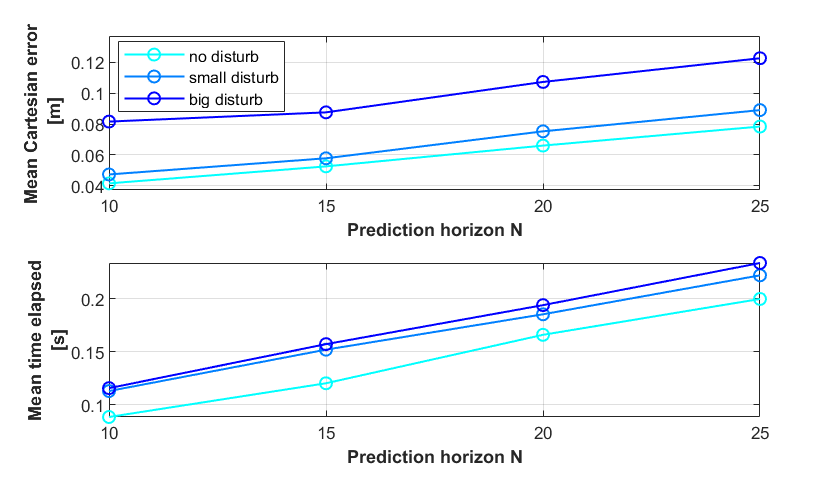
\includegraphics[scale=0.5]{base_curves_error}
	\centering
	\caption{Cartesian error and Optimization time when varying N}
	\label{base_curves_errors}
\end{figure}
\\In Figure \ref{base_curves} the trajectories that the mobile base follows are shown, considering different levels of random disturbances added to the input commands and considering different values of $N$. In Figure \ref{base_curves_errors} the relative errors and optimization times are shown. From these results we can notice that our controller is able to manage even high disturbances, but because of the limitation introduced by the parameterization of the input, it is more difficult for the optimizer to find a curve built on polynomial input commands that correctly approximates the given trajectory. This effect is even enlarged by the weighting profile of the cost function which give less importance to the accuracy of the first steps in the control horizon. Nevertheless Figure \ref{base_curves_errors} let us see that the time elapsed during the the optimization process does not increase exponentially like in traditional MPC, but it has just a slight increment.\\
\begin{figure}[!h]
	\centering
	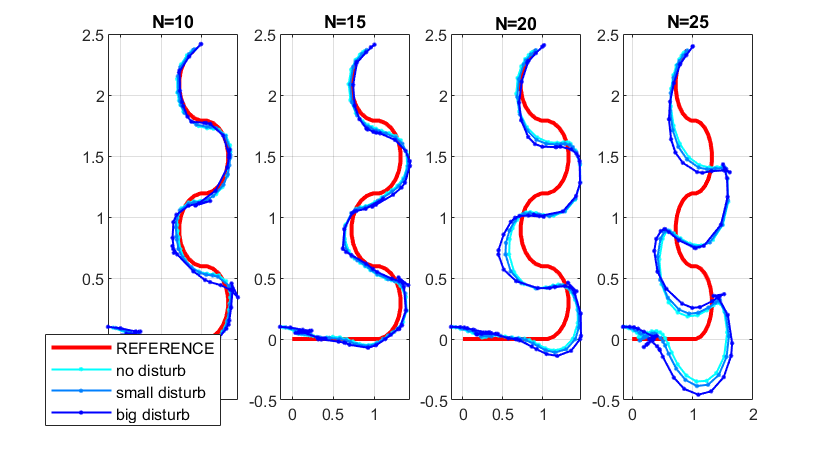
\includegraphics[scale=0.5]{base_curves2}
	\caption{Mobile platform trajectories with different N with a small-radius trajectory}
	\label{base_curves2}
\end{figure}
\begin{figure}[!h]
	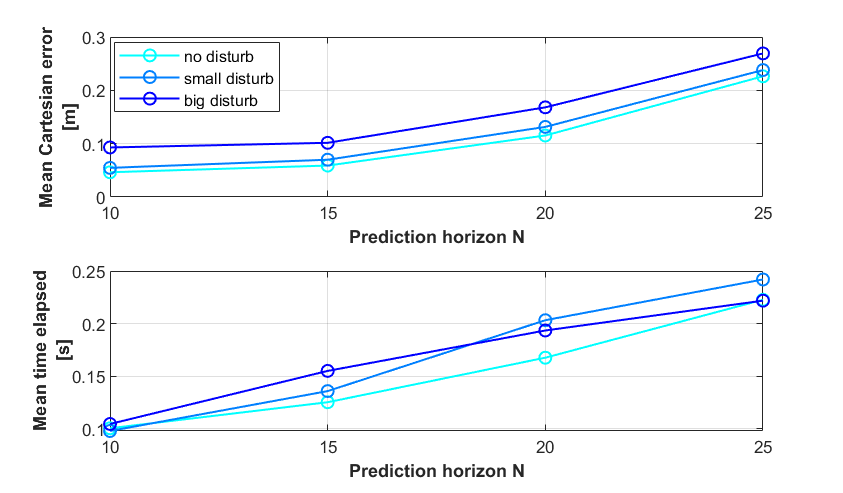
\includegraphics[scale=0.5]{base_curves_error2}
	\centering
	\caption{Cartesian error and Optimization time when varying N with a small-radius trajectory}
	\label{base_curves_errors2}
\end{figure}
To better understand the effect of a too high $N$ for complex trajectories, the same experiment has been run with a very similar trajectory but with a radius of the curves of $0.3$m instead of $0.6$m. The results of the simulations are found in Figures \ref{base_curves2} and \ref{base_curves_errors2}, where the effect of increasing $N$ is even more evident.
\begin{figure}[h!]
	\centering
	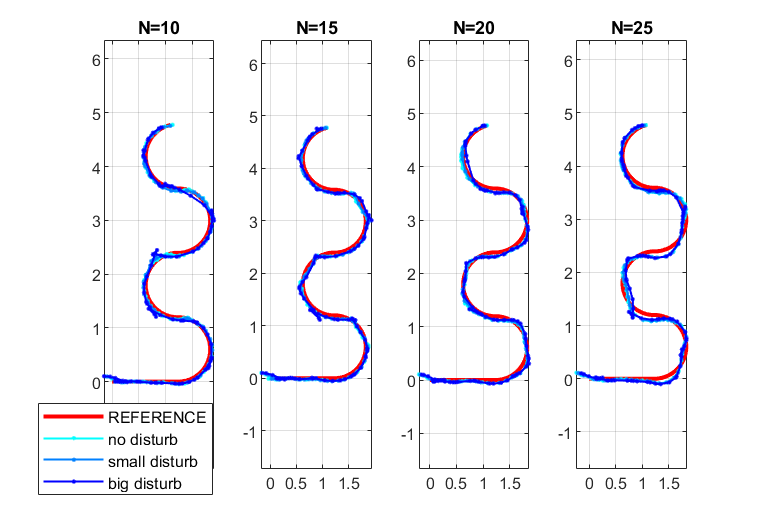
\includegraphics[scale=0.5]{base_curves3}
	\caption{Mobile platform trajectories with different N using 5th order polynomial inputs}
	\label{base_curves3}
\end{figure}
\begin{figure}[h!]
	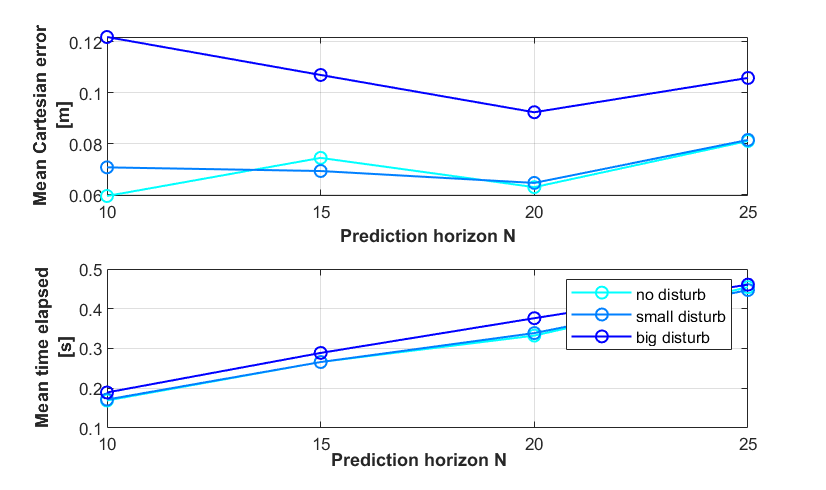
\includegraphics[scale=0.5]{base_curves_error3}
	\centering
	\caption{Cartesian error and Optimization time when varying N using 5th order polynomial inputs}
	\label{base_curves_errors3}
\end{figure}
\begin{figure}[h!]
	\centering
	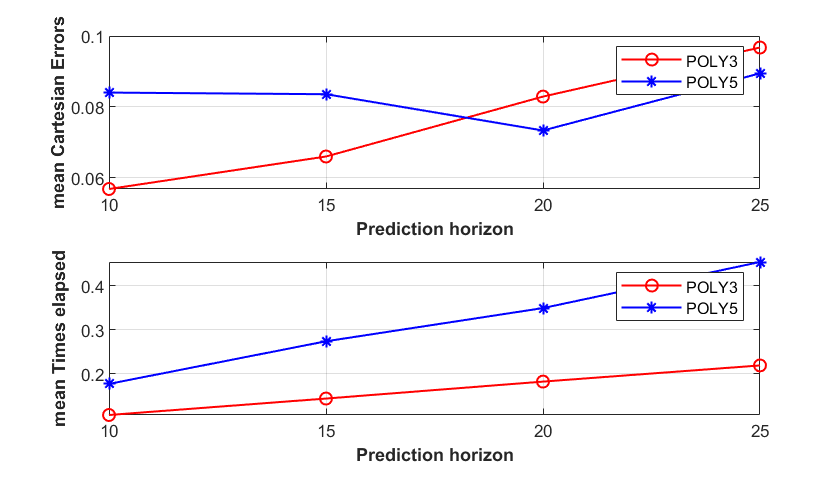
\includegraphics[scale=0.5]{base_curves_poly5}
	\caption{Comparison of errors and time of computation for 3rd and 5th order polynomial inputs}
	\label{base_curves_poly5}
\end{figure}
The previous tests have been performed describing the input commands $v$ and $\omega$ with a 3rd order polynomial. As Figures \ref{base_curves3} and \ref{base_curves_errors3} show, the effect of $N$ is lowered increasing the order of the input polynomial to 5. In Figure \ref{base_curves_poly5} a comparison between the two parameterizations in term of Cartesian error and elapsed times is shown; as was foreseeable, since the unknowns of the problem are more numerous having increased the polynomial order, the time needed for the computation of the optimization problem is higher. On the other hand, lower errors were expected with higher order polynomials; however a better performance in this sense is reached only at high $N$, since the optimizer can now found trajectories which stay closer to the reference trajectory.
\\\\
\begin{figure}[h!]
	\centering
	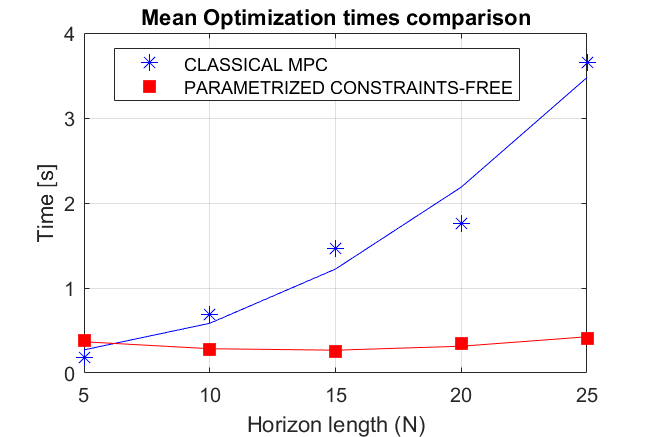
\includegraphics[scale=0.60]{solving_times_small}
	\caption{Solving time comparison}
	\label{solving_times}
\end{figure}
Once understood how some parameters affect the performance of the controlled system, we assessed the actual convenience of the presented approach running some simulations with the entire Mobile Manipulator system. We compared the solving times of our approach with the ones of a traditional MPC at different time horizon tracking a simple sinusoidal trajectory for the end effector position, in Figure \ref{solving_times}. It is easy to see the convenience of our approach, since the number of the unknowns that the optimizer has to find does not increase with $N$ and so with the dimension of the problem. In other words, the mean time needed to the optimizer to solve the MPC problem stays almost constant instead of increasing exponentially.\\
The following results have been obtained simulating the control of the Mobile Manipulator performing two types of motion, handling and grasping, since the controller is meant to be suitable for all the phases of a pick-and-transport task. The stage costs used in both cases have been explained in Chapter \ref{chapter6}.
\subsection{Mobile Manipulator Handling Simulations}
The entire Mobile Manipulator has been simulated performing a trajectory tracking in joint space, i.e. a custom trajectory for each coordinate of the base and for each manipulator joint has been given. Typically, in Mobile Manipulator handling tasks, the main objective is the locomotion of the base, while the arm can be kept stationary. For this reason a constant trajectory is asked to be tracked for the joints of the arm, while we have chosen to give the mobile base a trajectory involving high velocities to track. The results of the simulations are shown in Figures \ref{handling_traj} and \ref{handling_joints}. 
\begin{figure}[p]
	\centering
	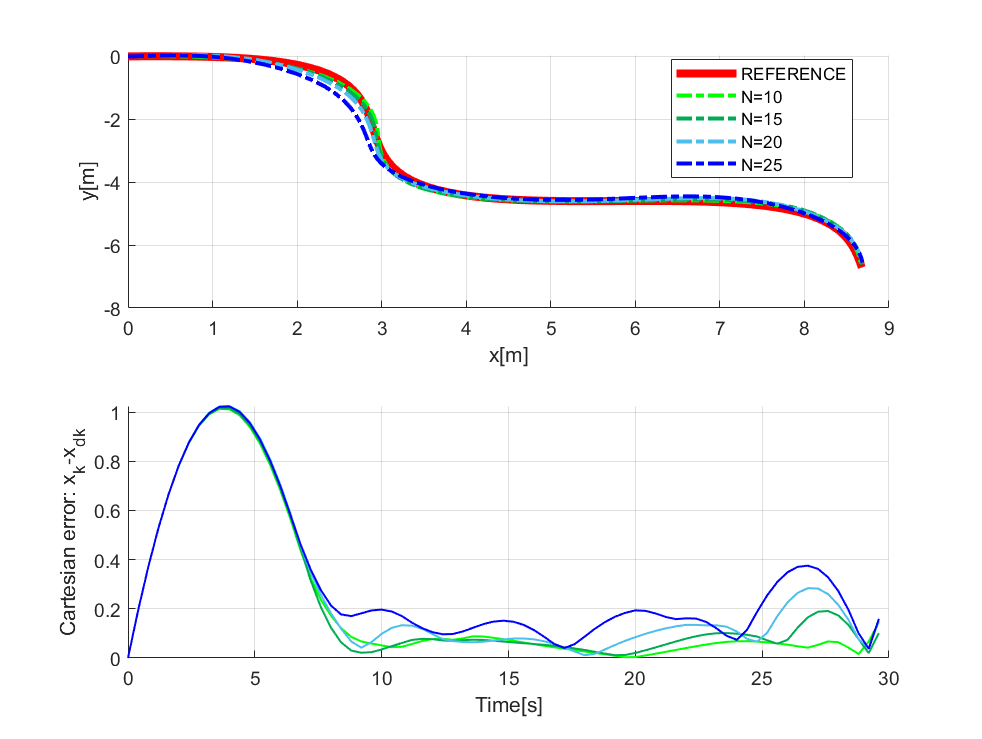
\includegraphics[scale=0.45]{handling_traj}
	\caption{Trajectory following of the mobile base during a Mobile Manipulator handling task}
	\label{handling_traj}
\end{figure}
\begin{figure}[p]
	\centering
	\includegraphics[scale=0.45]{handling_joints}
	\caption{Trajectory following of the joints during a Mobile Manipulator handling task}
	\label{handling_joints}
\end{figure}
A first consideration can be done on the Cartesian errors in tracking the mobile base motion. Indeed, in Figure \ref{handling_traj}, a peak of $1$ m of error can be seen at the very beginning of the trajectory. This is because the reference trajectory does not start with velocity equal to zero, while the robot starts from a stationary position; for this reason we can notice that the robot cuts the corner of the path to keep up with the reference trajectory. This "cutting the corner", actually, is the reason why increasing $N$, the errors in tracking the base position increase, as can also be seen in Figure \ref{handling_traj}. A second consideration is done on the trajectory tracking of the joint variables. Figure \ref{handling_joints} shows that our controller tracks very well a constant reference trajectory, varying the convergence to the constant value depending on $N$. This is because, even without imposing a constraint on the terminal state, our controller is driven to track exactly the reference value at the end of the prediction horizon; having kept the time step $T$ constant in all the simulations, a smaller time horizon leads to more reactive responses of the state.
\begin{figure}[p]
	\centering
	\includegraphics[scale=0.53]{end_effector_tests}
	\caption{End effector pose trajectory following with different N }
	\label{end_effector_tests}
\end{figure}
\begin{figure}[p]
	\centering
	\makebox[\textwidth][c]{\includegraphics[scale=0.47]{control_actions_SIM}}
	\caption{Control actions values over time. Boundary constraints are represented with the dashed lines}
	\label{control_actions_SIM}
\end{figure}
\subsection{Mobile Manipulator Grasping Simulations}
The entire Mobile Manipulator has then been simulated performing an EE position and orientation trajectory tracking on a sinusoidal 3D path. Since part of the trajectory lies outside the UR5 workspace, the Mobile Manipulator is asked to move in a synchronized fashion to correctly track the end effector pose. 
Results of these simulations are showed in Figure \ref{end_effector_tests}. The considerations made about previous tests still stand: the biggest limit of this controller is that it cannot find a trajectory defined with polynomial inputs that can stay close to too complex desired trajectories during long prediction horizons. The same effect has been seen keeping constant $N$ and increasing the time step $T$. Nonetheless, also in these results, it is possible to see how the optimization time has just a slight increment increasing $N$. In Figure \ref{control_actions_SIM} the control actions computed by the controller are shown to always satisfy the boundary constaints imposed.\\
In addition to the state and the control actions boundary constraints, others are been added to avoid self collision of the Mobile Manipulator. In particular, boundaries on the maximum and minimum arm joint values have to be satisfyied, along with a constraint on the minimum distance between the spheres embedding different parts of the robot. A brief simulation has been run to investigate wheter these self-collision constraint are satisfied; as shown in Figure \ref{self_collision}, giving the end effector a trajectory to folllow colliding with the mobile platform, the spheres embedding the end effector and the base never interpenetrate due to the given constraints.
\begin{figure}[t]
	\centering
	\includegraphics[scale=0.55]{self_collision_test}
	\caption{Tracking a self colliding trajectory}
	\label{self_collision}
\end{figure}
\\
We have described the results of simulations in two different tasks, having good performances controlling the robot in both situations. However a brief consideration on the passage from one control law to the other has to be done. Since both control laws are stable, this passage does not imply any instability ????????
\section{Physical experiments results}
\begin{floatingfigure}[l]{.3\textwidth}
	\centering
	\includegraphics[scale=0.03]{robot_marker}
	\caption{Aruco Markers positioning on ADAMMS\label{robot_marker}}
\end{floatingfigure} 
\begin{figure}[h!]
	\centering
	\includegraphics[scale=0.4]{img_real_exp.png}
	\caption{ADAMMS Experiments}
	\label{img_real_exp}
\end{figure}

Thanks to the results coming from simulations we were able to properly tune all the MPC parameters and weights in order to test the Mobile Manipulator in analogous tasks of handling and grasping tracking pre-planned reference trajectories. The latter do not involve high speeds for the mobile base for two main reasons: first of all, since the controller has been developed on Matlab/Simulink, even with the improvements we proposed, the commercial solver we used is still not suitable for fast online optimization processes. Therefore, being bound by the software availability point of view, we had to keep an high time step $T$, resulting in very distant way-points defining the base trajectory when the base speed is high. The other reason is related to available hardware.
The only measures of the position of the mobile platform are given from the odometry measurements of the platform itself, which are not reliable at high speeds because they do not consider the slipping of the wheels. Tests with different measuring systems like Aruco Markers localization, as in Figure \ref{robot_marker}, with cameras placed on the ceiling have been carried out, but the flickering of the image did not allow a fairly good measure.\\
Thence, experiments have been performed with $N=10$ and choosing $T=0.4\ s$.
\\\\
\subsection{Movement of the system toward grasping area}

The presented controller has been tested to perform handling operations tracking a fixed position for the arm joints and a given trajectory for the mobile base. This approach allows the controller to solve faster the optimization problem. For these experiments the initial position of the system was random and not belonging to the desired trajectory. The cost function used to solve this problem combines the error due to the base position $h_4$ and the error due to arm position in joints space $h_5$ as presented in \ref{chapter5}. The control horizon ($N$) used for this experiments has been setted equal to $10$, chosen after simulation results. In Figure \ref{hand_real1} the desired and the real performed trajectory of the base are shown.

	\begin{figure}[h!]
	\centering
	\includegraphics[scale=0.25]{empty.png}
	\caption{Base motion during grasping}
	\label{hand_real1}
	\end{figure}  

	\begin{figure}[h!]
	\centering
	\includegraphics[scale=0.25]{empty.png}
	\caption{Base error during handling}
	\label{err_hand_1}
	\end{figure}  

It is possible to notice, looking at the error graph in Figure \ref{err_hand_1}, that the base track properly the given trajectory. In Figure \ref{joint_pos_handl} joints position is given and compared to the desired one and it is possible to notice that, given that we are requiring a fixed position, the response of each joint is the response to a step input. 

	\begin{figure}[h!]
	\centering
	\includegraphics[scale=0.25]{empty.png}
	\caption{Joint position during handling}
	\label{joint_pos_handl}
	\end{figure}  




\subsection{Trajectory tracking in grasping operation}

The controller has been tested to perform grasping operations tracking EE trajectories as position and orientation in time as well as a desired motion of the base. For these experiments the system shows a response comparable to the model used in simulation. Anyway, considering the errors due to the positioning system of the base, as mentioned before, the system did not allow to be tested at high speed. The time chosen to perform this task has been setted between $35$ and $45 s$ according to the choice of $T$. 

	\begin{table}[]
	\centering
	\begin{tabular}{|l|l|l|ll}
	\cline{1-2}
	\multicolumn{2}{|l|}{ \textbf{Parameters} }	\\ \cline{1-2}
	$N$     				&  $10$ 	      					\\ \cline{1-2}
	$T$     				&  $0.4\ s$  	      					\\ \cline{1-2}
	$b$     				&  $3$ 	      						\\ \cline{1-2}
	$w_1$    				&  $1e6$       						\\ \cline{1-2}
	$w_2$    				&  $50$       						\\ \cline{1-2}
	$w_3$    				&  $1e5$       						\\ \cline{1-2}
	$w_4$    				&  $5e3$       						\\ \cline{1-2}
	$w_5$    				&  $0$      						\\ \cline{1-2}
	\end{tabular}
	\quad
	\begin{tabular}{|l|l|l|ll}
	\cline{1-3}
	\textbf{Constraints}    	& \textbf{min} 					& \textbf{max}			\\ \cline{1-3}
	$x_b$		 			 		&  -0.15 $m$ 					&  3.00 $m$ 			\\ \cline{1-3}
	$y_b$		 			 		&  -2.60 $m$ 					&  0.20 $m$ 			\\ \cline{1-3}
	$\theta_b$ 			 		&  -$\infty$  					&  +$\infty$ 			\\ \cline{1-3}
	$\Theta_1$ (Base)			&  -350°  						&  350° 				\\ \cline{1-3}
	$\Theta_2$ (Shoulder)		&  -180° 						&  0°		 			\\ \cline{1-3}
	$\Theta_3$ (Elbow) 			&  -140° 						&  140°		 			\\ \cline{1-3}
	$\Theta_4$ (Wrist1) 		&  -180° 						&  0°		 			\\ \cline{1-3}
	$\Theta_5$ (Wrist2)			&  -140° 						&  97°		 			\\ \cline{1-3} 
	$\Theta_6$ (Wrist3) 		&  -357° 						&  357°		 			\\ \cline{1-3}
	$\dot{v}$ 			 		&  -0.1 $m/s^2$					&  -0.1 $m/s^2$ 		\\ \cline{1-3}
	$\dot{\omega}$		 		&  -0.1 $rad/s^2$ 				&  -0.1 $rad/s^2$		\\ \cline{1-3}
	$\dot{\Theta}_{1,\dots,6}$	&  -0.2 $rad/s$					&  -0.2 $rad/s$ 		\\ \cline{1-3}
	\end{tabular}
	\caption{Experiment Parameters}
	\label{tableparam1}
	\end{table}
	The gripper used in the experiments is a Robotiq 2-Finger 85mm for Universal Robots. The instant at which the gripper has to be closed was defined offline and the communication ensured through a ROS node. In Figure \ref{seq_robot} the phisical system performing grasping during experiments is shoown.
	\begin{figure}[h!]
	\centering
	\includegraphics[scale=0.3]{seq_robot.png}
	\caption{ADAMMS Experiments}
	\label{seq_robot}
	\end{figure}
	The first experiment's results, performed with a linear parameterization for the arm joints are obtained using the parameters shown in Table \ref{tableparam1}. As can be seen the weight for the solution of the optimization problem has been chosen higher for the EE pose than for the base error. This choice lies in what is the aim of the performed task: since we are interested in grasp an object, the error we are more interested in is the pose of the end effector. Giving a desired position and orientation for the base only helps in defining the cost function properly. In fact, as mentioned in \ref{chapter4} the high redundancy of Mobile Manupulators is usually managed adding secondary tasks to be performed like maximization of manipulability index. 
	In Figure \ref{traj_ee1} the performed trajectory is shown in a 3D graph. 
	\begin{figure}[h!]
	\centering
	\includegraphics[scale=0.36]{traj_ee1.png}
	\caption{EE position during grasping}
	\label{traj_ee1}
	\end{figure}
	The results are then compared in Figure \ref{traj_ee1_comp} with the trajectory performed in simulation. The position and orientation of the EE are measured through the positioning system of the base presented in \ref{chapter6} and then using forward kinematics to compute position of the end effector. 
	\begin{figure}[h!]
	\centering
	\includegraphics[scale=0.45]{traj_ee1_comp.png}
	\caption{EE position comparison during grasping}
	\label{traj_ee1_comp}
	\end{figure}
	The trajectories in \ref{traj_ee1_comp} show that the system behaviour is close to the simulated one, this confirm the accuracy of the model. We will now analize the errors in performing this trajectory with respect to the desired one.  
	Given that we are interested in a tracking problem, i.e. the system has to be in the correct position at the right instant, and that the controller works at a fixed frequency $f_c=\frac{1}{T}$, the number of the given points $x_d$ implies that we are referring to a trajectory and not to a path. For this reason the offline planned desired points have to be generate accorging to velocity and acceleration requirements. 
	In Figure \ref{error_xyz1} absolute errors in $x$,$y$ and $z$ position of the EE are shown for a linear parameterization of the arm joints velocities.
	\begin{figure}[h!]
	\centering
	\includegraphics[scale=0.4]{error_xyz1.png}
	\caption{EE position errors during grasping}
	\label{error_xyz1}
	\end{figure}
	\begin{figure}[h!]
	\centering
	\includegraphics[scale=0.4]{error_orient1.png}
	\caption{EE orientation errors during grasping}
	\label{error_orient1}
	\end{figure}

	Errors in orientation are shown in Figure \ref{error_orient1}. Orientation is important in grasping operation because trajectories have to be planned according to the part to be handled. What is possible to see from \ref{error_xyz1} and \ref{error_orient1} is that the more the points are close eachother, that means low speeds, the more the tracking errors are small. In Figure \ref{base_err_exp1} the base motion and errors are shown and it is possible to notice that the errors are higher than the EE position. This is due to the fact that, for this task, we are weighting more the EE error than the base error.
	The experiments has been performed successfully grasping different objects requiring different orientation approach for the EE.  
	\begin{figure}[h!]
	\centering
	\includegraphics[scale=0.4]{base_err_exp1.png}
	\caption{Base motion during grasping}
	\label{base_err_exp1}
	\end{figure}
	In Figure \ref{err_num_base} errors on the cartesian base position of the base are reported for grasping experiment while in Figure \ref{vel_real} acceleration of the base in it's longitudinal and angular components and velcities of the joints are reported and compared to the given constraints.
	\begin{figure}[h!]
	\centering
	\includegraphics[scale=0.2]{empty.png}
	\caption{Base cartesian error during grasping}
	\label{err_num_base}
	\end{figure}
	\begin{figure}[h!]
	\centering
	\includegraphics[scale=0.20]{empty.png}
	\caption{Control actions constraints}
	\label{vel_real}
	\end{figure}
	To understand the performance in manipulability maximization we will show the value of $sin(\Theta_3)$ which is a good index of how far the arm is from it's singularities. In figure \ref{man_real1} is it possible to notice that this value is well bounded and minimized as was possible to notice during the experiments.
	\begin{figure}[h!]
	\centering
	\includegraphics[scale=0.25]{empty.png}
	\caption{Manipulability during grasping}
	\label{man_real1}
	\end{figure}

	\fix{aggiungere qualcosa sul solutore}
%!TEX root = Thesis_main.tex

\chapter{Conclusions}
\label{conclusions}

The developed high level controller for the presented Mobile Manipulator, together with results from simulation and physical experiments, requires some considerations on the effectiveness of the presented approach. As shown in Chapter \ref{chapter7} our approach gives improvements in reducing solving time with respect to a standard nonlinear MPC with piecewise control action and terminal constraint. In particular, the dependence of the computational effort on $N$ is reduced. Anyway in Chapter \ref{chapter7} also drawbacks of this approach are presented like the dependence on the number of parameters and the affect of the increasing weight profile for the cost function. The overall results show an approach that, for many application, can represent a step towards online developing of nonlinear MPC for fast application. The usage of a nonlinear model based controller, as mentioned before, allows to represent and control complex systems taking into account many degrees of freedom and coupling effects between them but introduces further limitations. Nonlinearities in the model lead to a non-convex problem, local minima existence, higher computational effort and difficulties in assessing stability. The advantage of a nonlinear model instead of using linearization techniques is then a key question, in fact very good results can be nowdays acheived linearizing the model of the system obtaining a faster controller with all the benefit that follow. Nevertheless, the complexity of systems as well as the increasing requirements in performing complex task requires exact models and this implies high nonlinearities. Furthermore, the increasing computational capability of control units as well as research works on new techniques to treat optimization problems is moving towards solving nonlinearities issues. Summarizing, the high level controller developed based on the presented approach gives it's contribution trying to reduce the computational effort towards fast NMPC application but to properly understand its capabilities future works are needed.

\section{Future Works}

The presented work propose an approach towards fast nonlinear model predictive control for online application but leaves a consistent number of aspects that needs to be studied in deep. 
Indeed, the developed implementation of this approach can be improved optimizing the code using stand alone C++ code to be run in ROS. Futhermore, the presence of local minima in the cost function minimization can be studied and a better understanding of the affection of different terms in the cost function is required for this. The capabilities of the available sensors for the positioning system of the base affect significantly the position of the end effector and so the accuracy of the entire system. Because of that, the performances in real applications can be improved developing a better estimation system using filtering techniques. Grasping, as presented in this work, can be improved studing different approaches that can be integrated with the controller as presented, though giving optimized pre-planned trajectories can be a sufficient solution. The setup of the solver used (IPOPT) can be analized and customized to reduce again the solving times. Moreover, this approach can be tested with a linearized system to understand if the same benefits are present in linear MPC approaches, i.e. if the dipendece on $N$ is reduced. Finally stability of this approach has to be studied in deep to understand if there is a closed form to proof the stability of this approach depending on the exponent $b$ or if the stability is necessarily dependent on solver performances.


% - dire del codice che si può implementare meglio \\
% - dire che si possono provare a verificare dove e come avvengono minimi locali \\
% - dire che si possono fare delle prove con della sensoristica migliore \\
% - dire che si può introdurre grasping fatto meglio studiando le traiettorie corrette \\
% - dire che se il solutore si può settare meglio (tolleranze e componenti del solutore commerciale) \\
% - dire che si può provare ad applicare questo approccio a linear MPC per ridurre la dipendenza sull'N \\

\appendix
\renewcommand{\thesection}{\Alph{section}}
\renewcommand{\thefigure}{\thesection.\arabic{figure}}
\renewcommand{\thetable}{\thesection.\arabic{table}}
%!TEX root = Thesis_main.tex
\chapter*{Appendices}
\clearpage
\addcontentsline{toc}{chapter}{Appendices}
\section{Super Mega Bot Datasheet}
\label{AppA}

\begin{figure}[h]
	\begin{center} 
		\subfigure[Supermegabot]{
		\includegraphics[scale=0.43]{SuperMegaBot}
		\centering
		\label{fig:SuperMegaBot}}
		\qquad
		\subfigure[Wiring scheme]{
		\includegraphics[scale=0.43]{SMBwires}
		\centering
		\label{SMB Wiring}}
		\caption{SMB Data}
	\end{center}
\end{figure}

Its base model comes with:\\
•	Chassis: Powder Coated Steel and Aluminum \\
•	Dimensions: 84cm L x 84cm W x 40.64cm H, Weight: 109 kg\\
•	Drive: Four Electric Motors\\
•	Load Capacity: 113,5 kg\\
•	Speed Controllers: RoboteQ 2x VDC2450\\
•	Speed: 0-16 km/h \\
•	Suspension: Rigid\\
•	Tires: Interchangeable, Pneumatic, 40.64cm Diameter Turf Tires\\
\url{https://www.youtube.com/watch?v=3X8IWnR1QDI}

%%%%%%%%%%%%%%%%%%%%%%%%%%%%%%%%%%%%%%%%%%%%%%%%%%%%%%%%%%%%%%%%%%%%%%%%%%%%%%%%%%%%%%%%%%%%%%%%%%%%%%%%%%%%%%%%%%%%%%



% \begin{figure}[!th]
% 	\begin{center} 
% 		\centerline{\includegraphics[scale=0.9]{ur5_en_V2}}
% 		\label{SMB Wiring} 
% 	\end{center}
% \end{figure}
\includepdf[pagecommand={\section{UR5 Datasheet}}, offset=15 0]{ur5_en_V2.pdf}
\label{AppB}

%%%%%%%%%%%%%%%%%%%%%%%%%%%%%%%%%%%%%%%%%%%%%%%%%%%%%%%%%%%%%%%%%%%%%%%%%%%%%%%%%%%%%%%%%%%%%%%%%%%%%%%%%%%%%%%%%%%%%%

\section{Interior Point OPTimizer (IPOPT)}
\label{AppC}



IPOPT (\underline{I}nterior \underline{P}oint \underline{Opt}imizer,
pronounced ``Eye--Pea--Opt'') is an open source software package for
large-scale nonlinear optimization. It can be used to solve general
nonlinear programming problems of the form
%\begin{subequations}\label{NLP}
\begin{eqnarray*}
\min_{x\in\RR^n} &&f(x) \label{eq:obj} \\
\mbox{s.t.} \;  &&g^L \leq g(x) \leq g^U \label{eq:constraints}\\
                &&x^L \leq x \leq x^U, \label{eq:bounds}
\end{eqnarray*}
%\end{subequations}
where $x \in \RR^n$ are the optimization variables (possibly with
lower and upper bounds, $x^L\in(\RR\cup\{-\infty\})^n$ and
$x^U\in(\RR\cup\{+\infty\})^n$), $f:\RR^n\longrightarrow\RR$ is the
objective function, and $g:\RR^n\longrightarrow \RR^m$ are the general
nonlinear constraints.  The functions $f(x)$ and $g(x)$ can be linear
or nonlinear and convex or non-convex (but should be twice
continuously differentiable). The constraints, $g(x)$, have lower and
upper bounds, $g^L\in(\RR\cup\{-\infty\})^m$ and
$g^U\in(\RR\cup\{+\infty\})^m$. Note that equality constraints of the
form $g_i(x)=\bar g_i$ can be specified by setting
$g^L_{i}=g^U_{i}=\bar g_i$. \\

More information aboit Interior point method can be found in \cite{polik2010interior}.
IPOPT technical informations can be found at \url{https://projects.coin-or.org/Ipopt}.

% In the following table the specifications given by Universal Robots are stated. 
% \begin{table}
% 	\begin{tabular}{p{4cm} | p{3cm} p{3cm}}
% 		\hline
% 		Performance & \multicolumn{2}{l}{ } \\
% 		\hline \hline
% 		Repeatibility & \multicolumn{2}{l}{$\pm$ 0.1 mm} \\
% 		Ambient temperature range & \multicolumn{2}{l}{0-50°} \\
% 		Power Consumption  & \multicolumn{2}{l}{Min 90W, Typical 150W, Max 325W} \\
% 		Collaboration operation & \multicolumn{2}{l}{15 advanced adjustable safety functions} \\
% 		\hline \hline
% 		Specifications & \multicolumn{2}{l}{ }\\
% 		\hline \hline 
% 		Payload & \multicolumn{2}{l}{5 kg} \\
% 		Reach & \multicolumn{2}{l}{850 mm} \\
% 		Degrees of freedom & \multicolumn{2}{l}{6 rotating joints} \\
% 		Programming & \multicolumn{2}{l}{Polyscope graphical user interface on 12 inch touchscreen} \\
% 		\hline \hline
% 		Movement & & \\
% 		\hline 
% 		& Working range & Maximum speed \\
% 		\hline \hline
% 		Base & $\pm$ 360°  & $\pm$ 180°/sec \\
% 		Shoulder & $\pm$ 360° & $\pm$ 180°/sec \\
% 		Wrist1 & $\pm$ 360° & $\pm$ 180°/sec \\
% 		Wrist2 & $\pm$ 360° & $\pm$ 180°/sec \\
% 		Wrist3 & $\pm$ 360° & $\pm$ 180°/sec \\
% 		Typical tool & & 1m/sec \\
% 		\hline \hline
% 		Physical & \multicolumn{2}{l}{ }\\
% 		\hline \hline
% 		Footprint & \multicolumn{2}{l}{\o 149mm} \\
% 		Materials & \multicolumn{2}{l}{Aluminium, PP Plastics} \\
% 		Weight (with cable) & 18.4 kg 
% 	\end{tabular}
% \end{table}

\cleardoublepage

%----Appendice tabelle e figure----

\addcontentsline{toc}{chapter}{\listfigurename} %\dotfill aggiungerlo per i puntini
\listoffigures

\cleardoublepage

\addcontentsline{toc}{chapter}{\listtablename}
\listoftables



\leavevmode\thispagestyle{empty}\newpage

\phantomsection
\renewcommand{\bibname}{References}
\addcontentsline{toc}{chapter}{References}
\bibliographystyle{ieeetr}
\bibliography{references}

%\nocite{*}

%\appendix

%\pagestyle{fancy} 
%\fancyfoot{}                                               
%\renewcommand{\chaptermark}[1]{\markboth{\appendixname\ \thechapter.\ #1}{}} 
%\renewcommand{\sectionmark}[1]{\markright{\thesection.\ #1}}         
%\fancyhead[LE,RO]{\bfseries\thepage}    
                                       
%\fancyhead[RE]{\bfseries\leftmark}    
%\fancyhead[LO]{\bfseries\rightmark}     
%\renewcommand{\headrulewidth}{0.3pt} 




\end{document}





